%\documentclass[sigconf, titlepage, twoside]{acmart}
\documentclass[12pt,titlepage, twoside]{article}
%\usepackage{titlesec}

% language stuff
\usepackage{german}           % deutsche Überschriften etc.
\usepackage[utf8]{inputenc} % direkte Eingabe von Umlauten

% Layout-Einstellungen
\usepackage{parskip}          % Abstand statt Einrückung
\frenchspacing                % no extra space after periods
\usepackage{parskip}          % paragraph gaps instead of indentation
\usepackage{times}            % default font Times
\tolerance=9000               % avoid words across right border

% miscellaneous
\usepackage{graphicx}         % graphics
\usepackage{subcaption}       % subfigures
\usepackage{hhline}           % double lines in tables
\usepackage{amsfonts}         % real numbers etc.
\usepackage[rightcaption]{sidecap} % figure captions on the right (optional)
\usepackage{hyperref}         % for URLs
\usepackage{listings}         % for code samples
\usepackage{fancyhdr}         % for header line
\usepackage{lastpage}         % for last page count

\usepackage{makecell}

\usepackage{xcolor}           % Code highligting

\usepackage{amsmath}

\colorlet{punct}{red!60!black}
\definecolor{background}{HTML}{EEEEEE}
\definecolor{delim}{RGB}{20,105,176}
\definecolor{string}{RGB}{0,0,255}
\colorlet{numb}{magenta!60!black}

\lstdefinelanguage{json}{
    basicstyle=\normalfont\ttfamily,
    %numbers=left,
    %numberstyle=\scriptsize,
    stepnumber=1,
    numbersep=8pt,
    showstringspaces=false,
    breaklines=true,
    frame=lines,
    stringstyle=\ttfamily\color{string},
    %backgroundcolor=\color{background},
    literate=
     *{0}{{{\color{numb}0}}}{1}
      {1}{{{\color{numb}1}}}{1}
      {2}{{{\color{numb}2}}}{1}
      {3}{{{\color{numb}3}}}{1}
      {4}{{{\color{numb}4}}}{1}
      {5}{{{\color{numb}5}}}{1}
      {6}{{{\color{numb}6}}}{1}
      {7}{{{\color{numb}7}}}{1}
      {8}{{{\color{numb}8}}}{1}
      {9}{{{\color{numb}9}}}{1}
      {:}{{{\color{punct}{:}}}}{1}
      {,}{{{\color{punct}{,}}}}{1}
      {\{}{{{\color{delim}{\{}}}}{1}
      {\}}{{{\color{delim}{\}}}}}{1}
      {[}{{{\color{delim}{[}}}}{1}
      {]}{{{\color{delim}{]}}}}{1},
}
%
%\newcommand{\imageSizeTwo}{0.49\textwidth}
%\newcommand{\imageSizeTwoHeight}{7.5cm}
\newcommand{\imageSizeTwo}{0.35\textwidth}
\newcommand{\imageSizeTwoHeight}{4.5cm}
\newcommand{\imageSizeThree}{0.3\textwidth}
\newcommand{\imageSizeThreeHeight}{5cm}
\newcommand{\imageWidthFour}{width=2cm height=2cm}

% Hier bei Bedarf die Seitenränder einstellen
\usepackage{geometry}
%\geometry{a4paper}
\geometry{a4paper, top=3.5cm, bottom=2.5cm} 

% Kopf- und Fußzeile
\fancyhead{} % clear all header fields
\fancyhead[RO,LE]{\leftmark}

%%%%%%%%%%%%%%%%%%%%%%%%%%%%%%%%%%%%%%%%%%%%%%%%%%%%%%%%%%%%%%
\begin{document}

%-------------------------------------------------------------
\begin{titlepage}
%-------------------------------------------------------------
\begin{center}
{\Large\bf Analyse von Pflanzenwachstum auf Basis von 3D-Punkwolken}\\[3cm]

{\bf Masterarbeit}\\
zur Erlangung des Grades {\em Master of Science}\\[1.5cm]

an der\\
Hochschule Niederrhein\\
Fachbereich Elektrotechnik und Informatik\\
Studiengang {\em Informatik}\\[3cm]

vorgelegt von\\
Jakob Görner\\
1003660\\[3cm]
Datum: \today\\[3cm]

Prüfer: Prof.~Dr.~Regina Pohle-Fröhlich\\
Zweitprüfer: Prof.~Dr.~Christoph Dalitz

\end{center}
\end{titlepage}

\pagestyle{empty}
\cleardoublepage

\newpage


%-------------------------------------------------------------
\section*{Eidesstattliche Erklärung}
%-------------------------------------------------------------
\begin{tabbing}
Name: \hspace{4em}\= Jakob Görner\\
Matrikelnr.: \> 1003660\\
Titel: \> Analyse von Pflanzenwachstum auf Basis von 3D-Punkwolken
\end{tabbing}

Ich versichere durch meine Unterschrift, dass die vorliegende
Arbeit ausschließlich von mir verfasst wurde.
Es wurden keine anderen als die von mir angegebenen Quellen und Hilfsmittel
benutzt.

Die Arbeit besteht aus \pageref{LastPage} Seiten.

\vspace{8ex}
\begin{tabbing}
\underline{\hspace{16em}} \hspace{3em}\= \underline{\hspace{14em}} \\
Mönchengladbach, \today \> Unterschrift
\end{tabbing}

\newpage
%\begin{abstract}
%-------------------------------------------------------------
\section*{Zusammenfassung}
%-------------------------------------------------------------
In dieser Arbeit soll eine Anwendung zum Analysieren von Pflanzen-Wachstum und weiteren Merkmalen des Wachstumsprozesses einer Pflanze erstellt werden. 
Es soll aus einer Reihe von Bildern einer Pflanze, die mit einer gängigen Smartphone-Kamera aufgenommen sind, eine Punkwolke erzeugt werden. 
Aus der Punktwolke sollen die Punkte die zur Pflanze gehören extrahiert werden. 
Die extrahierten Punkte werden zur weiteren Analyse in Stamm- und Blatt-Punkte segmentiert.
Des weiteren sollen Werte, wie das Wachstum der Pflanze, ermittelt werden. Hierzu müssen mehrere Punktwolken über Zeit miteinander verglichen werden.
Die Anwendung soll mit möglichst wenig Bildern auskommen um den Datentransfer zu minimieren.

\setcounter{page}{1}
%-------------------------------------------------------------
\section*{Abstract}
%-------------------------------------------------------------
Development of an application made to analyse plant growth over time and further characteristics of a plant represented as a point cloud. 
The point cloud should be generated out of a set of images of the plant, taken with a common smartphone.
First the points representing the plant have to be extracted first.
After this the remaining point cloud should be splitted in leave and stem points to count leaves and analyse the stem further. 
Also other characteristics as the hight should be analysed. For this reason multiple point clouds has to be compared over time.
The application should use as few pictures as possible to reduce the amount of transfered data.

%\end{abstract}
\newpage

\pagestyle{plain}
\tableofcontents
\newpage

%-------------------------------------------------------------
% default a), b), c) numbering
\renewcommand{\labelenumi}{\alph{enumi})} 

%=============================================================


\section{Motivation}
%-------------------------------------------------------------
\label{sec:einleitung}
Diese Arbeit wird im Rahmen eines Projekts der Hochschule Niederrhein (Krefeld, Deutschland) mit den Universitäten Makerere University (Kampala, Uganda) und Central University of Technology (Bloemfontein, Südafrika) durchgeführt.
%Das Projekt beschäftigt sich in erste Linie mit der Sicherstellung von nachhaltiger Nahrungsproduktion.
Im Rahmen dieser Arbeit soll eine Anwendung entstehen, die in den beiden Ländern für Kleinbauern zum Einsatz kommen soll.
Die Anwendung soll mit nichtinvasiven Methoden zur Unterstützung bei der selektiven Züchtung eingesetzt werden, um Erträge und somit auch Gewinnmargen zu erhöhen und damit zur Ernährungssicherheit beizutragen.
Dies ist nötig, da es im Rahmen der derzeitigen Klimaveränderungen zu höheren Ernteausfällen durch Dürren kommt \cite{droughts}, die durch reinen Einsatz von indigenem Wissen nicht zu kompensieren sind.

Um diesem Ziel näher zu kommen soll in dieser Arbeit eine Software entwickelt werden, die es erlaubt Daten über den Wachstums-Prozess von Pflanzen zu sammeln. 
Diese soll als Grundlage für weitere Analysen wie das frühe Erkennen von Krankheitsbildern, Ertragsschätzungen oder Erkennen unzureichender Wachstumsraten der Pflanzen dienen.

Ziel ist es also eine Software zu schaffen, die es ermöglicht aus Bildern von Pflanzen 3D Punktwolken (Punktwolken) zu generieren und diese zu analysieren.
Es soll mit der zu entwickelnden Anwendung möglich sein, Aussagen über das Wachstum über Zeit, die Entwicklung der Blätter und der Stämme zu treffen. 
Mit diesen Daten sind Analysen möglich, die auf das Wachstum einer Pflanze unter bestimmten Bedingungen schließen lassen.
Hierbei gibt es besondere Anforderungen an den Prozess der Datengewinnung und Übertragung. Zum einem muss der Betrieb kostengünstig sein - das betrifft insbesondere den Endverbraucher.
Der Endverbraucher sollte möglichst wenig Datenmengen an den Server, der die Rechenkapazität bereit stellt, übertragen müssen. 
Das soll die Kosten auf Seiten der Kleinbauern gering halten.
Des weiteren muss die Datengewinnung mit einem Mobiltelefon oder einer anderen Kamera möglich sein. 
Spezielle Aufnahmegeräte, wie ein LIDAR-Scanner, die den Kleinbauern nicht schon zur Verfügung stehen sollen nicht nötig sein.

\newpage
\section{Stand der Technik}
%-------------------------------------------------------------
\label{sec:stand}
%Hier müssen Sie beschreiben wie die Situation vor Ihrem Beitrag war.
%Dazu gehören die Vorarbeiten anderer, auf denen Sie aufsetzen, die
%bisher eingesetzte Software oder Hardware und allgemeine
%bekannte Techniken, die in Ihrer Arbeit zum Einsatz kamen.
%
%In diesen Abschnitt gehören alle Aspekte, die zum Verständnis der
%Arbeit erforderlich sind, aber einem mit der Aufgabenstellugn nicht vertrauten
%fachkundigen Leser nicht zwangsweise bekannt sind.

Drei Kernprobleme müssen betrachtet werden, die für den Erfolg dieser Arbeit gelöst werden müssen. 
Zuerst muss aus einer Menge an Bildern eine Punktwolke generiert werden. 
Danach muss die Punktwolke segmentiert werden, um den Hintergrund zu entfernen und die einzelnen Teile der Pflanze, wie Blätter und Stiele, zu erkennen und weiter zu analysieren. 
Zuletzt müssen zwei Punktwolken einer Pflanze zu verschiedenen Zeitpunkten miteinander registriert werden, um Aussagen über das Wachstum einer Pflanze treffen zu können.

\subsection{Generierung einer 3D Punktwolke aus Bildern}
\label{sec:stand:pointcloud}

Generell kann man zwischen zwei Methoden der Generierung von Punktwolken unterscheiden, die jeweils verschiedene Verfahren beziehungsweise Techniken anwenden.

Die erste Methode nutzt Hardware wie LIDAR-Scanner \cite{lidar} um Punktwolken direkt zu erzeugen. Es gibt eine Reihe von Sensoren die das ermöglichen. 
Da der Großteil der Sensoren aus Kostengründen nicht in Frage kommt, sei hier nur noch der RGB-D-Sensor erwähnt. 
Dieser liefert neben den Farbwerten für ein Bild auch noch eine Tiefeninformation für jedes Pixel. In einigen Smartphone-Modellen wird bereits ein solcher Sensor verbaut \cite{rgbd_smartphones}.
Ein Nachteil bei RGB-D Sensoren ist aber, dass sie anfällig für Änderungen der Lichtverhältnisse sind, was gerade im Außenbereich häufig vorkommt.

Die andere Methode ist Structure from Motion (SfM), bei der die Punktwolke aus Bildern einer Szene aus verschiedenen Perspektiven generiert wird. 
Allgemein wird auf den zugrundeliegenden Bildern nach Merkmalen (Feature) gesucht die robust gegen Translation, Rotation, Skalierung und Beleuchtung seien sollten. 
Generell ist das Ermitteln von geeigneten Features in zwei Teile zu unterteilen, die Feature-Erkennung und die Feature-Beschreibung. 
Bei der Feature-Erkennung müssen geeignete Punkte im Bild als Kandidaten für Feature-Punkte ermittelt werden. 
Sind geeignete Kandidaten gewählt worden, müssen diese beschrieben werden, also ein Deskriptor für den Punkt gefunden werden. Hier kann man die bekanntesten Umsetzungen in zwei Bereiche unterteilen. 
Umsetzungen wie Scale Invariant Feature Transformation (SIFT) \cite{Sift} und Speeded Up Robust Features (SURF) \cite{SURF} beschreiben einen Feature-Punkt als einen Vektor, der aus Gradienten-Histogrammen um den Punkt herum gebildet wird.
Binary Robust Independent Elementary Features (BRIEF) \cite{BRIEF} und FAST and Rotated BRIEF (ORB) \cite{ORB} nutzen statt dessen einen binären Deskriptor um den Feature-Punkt zu beschreiben. 
Hierbei werden die Intensitäts-Differenzen bestimmter Punkt-Paare in einem Bereich um den Punk mit einem Schwellwert verglichen und so der binäre Deskriptor gebildet.

SIFT ist der wohl bekannteste Ansatz und wird häufig als Goldstandart verwendet um Verfahren miteinander zu vergleichen. Es hat allerdings den Nachteil, dass es zu langsam für Echtzeitanwendungen ist.
SIFT ermittelt die Kandidaten-Punkte im Kern mittels dem Difference of Gaussians Verfahren (DoG). DoG besteht aus drei Schritten. Im ersten Schritt wird auf das Bild in verschieden starken Stufen ein Weichzeichner (diskreter Gauß-Filter) angewandt.
Damit liegt das Bild mit zunehmend niedrigerem Kontrast vor. Zwischen den einzelnen Kontraststufen wird die Differenz ermittelt. Liegen die Differenzen vor kann nach Extrempunkten in den Differenzen gesucht werden.
Hierbei wird für jedes Pixel im Bild mit seinen direkten Nachbarn und denen in der vorherigen und nachfolgenden Stufe verglichen. Ist das Pixel ein Extrempunkt, wird es als Kandidat gewählt.
DoG wird auf mehreren Skalierungen des Bildes angewandt um Skalierungs-Invarianz zu erreichen.
Im Anschluss werden die Kandidaten gefiltert. Kandidaten, die einen niedrigen Intensitätswert haben oder eine Kante darstellen, werden hierbei ausgeschlossen.
Sind die Positionen der Features bekannt, kann der Feature-Vektor $f$ für den Punkt $p$ ermittelt werden. 
Um den Deskriptor für den Punkt $p$ zu berechnen werden zwei Größen benötigt. Zum einen die Skalierung, in der der Punkt ermittelt wurde - diese ist bereits bekannt - und die Orientierung des Punktes.
Um diese zu bestimmen werden in einem Bereich um den Punk $p$ die Gradienten berechnet und in ein Histogramm abgetragen. Der Histogramm-Eintrag mit dem größten Wert entscheidet die Orientierung des Punktes.
Sind Skalierung und Orientierung bekannt, wird ein Bereich auf Basis der beiden gewählt und in einen $16\times 16$ großen Bereich skaliert. 
Dieser Bereich wird in $16$ gleichgroße Bereiche unterteilt, für die jeweils ein Histogramm gebildet wird. 
Die Einträge beschreiben in $8$ diskreten Stufen die Orientierung der Punkte im jeweiligen Bereich. 
Die einzelnen Punkte tragen die Stärke des Gradienten im jeweiligen Bin des Histogramms ab.
Diese Histogramme bilden den Feature-Vektor $f$, der für den Vergleich genutzt wird.

SURF ist ähnlich aufgebaut wie SIFT, nur wird der genutzte Gauss-Filter durch Box-Filter, die besonders effizient berechnet werden, approximiert.
Des weiteren wird der Feature-Vektor anders gebildet. Mit beiden Anpassungen wird eine bessere Leistung erreicht.
Bei der Approximation des Gauss-Filters wird zuerst das Integral-Bild $I_\Sigma$ aus den Intensitätswerten $I$ des Bildes berechnet \ref{eq:sfm:surf:integral}.
\begin{equation}
    \label{eq:sfm:surf:integral}
    I_\Sigma (x,y) = \sum_{i=0}^{i\leq x}\sum_{j=0}^{j\leq y}I(i,j)
\end{equation}
Ist $I_\Sigma$ bekannt, kann die Intensitäts-Summe eines beliebigen rechteckigen Ausschnitts sehr effizient berechnet werden. 
Hierzu werden nur die Werte aus $I_\Sigma$ für die Eckpunkte $P_1$ - $P_4$ eines Ausschnittes $D$ benötigt.
Die Fläche für $D$ lässt sich dann mit $f(D)$ effizient berechnen \ref{eq:sfm:surf:f}.
\begin{equation}
    \label{eq:sfm:surf:f}
    f(D) = I_\Sigma(P1) + I_\Sigma(P4) - I_\Sigma(P2) - I_\Sigma(P3)
\end{equation}
Um den Gauss-Filter mit Box-Filtern zu approximieren, wird die Determinante der Hesse-Matrix genutzt. 
Um die approximierte Hesse-Matrix für einen Punkt $p$ mit der Skalierung $s$ zu bilden, muss man die zweite Ableitung der Gauss-Funktion nach $x$, $y$ und $xy$ mit Box-Filtern approximieren \ref{eq:sfm:surf:h}.
\begin{equation}
    \label{eq:sfm:surf:h}
    H_{approx.}(p,s) = \left( \begin{smallmatrix} D_{xx}(p,s)&D_{xy}(p,s)\\ D_{xy}(p,s)&D_{yy}(p,s) \end{smallmatrix} \right)
\end{equation}
Die Determinante der Hesse-Matrix kann dann wie in Gleichung \ref{eq:sfm:surf:det} berechnet werden, wobei $w\approx 0.9$ ist und den Fehler der Approximation minimieren soll.
\begin{equation}
    \label{eq:sfm:surf:det}
    det(H_{approx.}) = D_{xx}D_{yy}-(wD_{xy})^2
\end{equation}
Ein Beispiel für die Box-Filter ist in Abbildung \ref{fig:surf:filter} zu sehen. Sowohl die verschiedenen Gauss-Stufen, als auch die verschiedenen Skalierungs-Stufen werden durch ein Vergrößern der Filter-Maske erreicht.
\begin{figure}
    \centering
    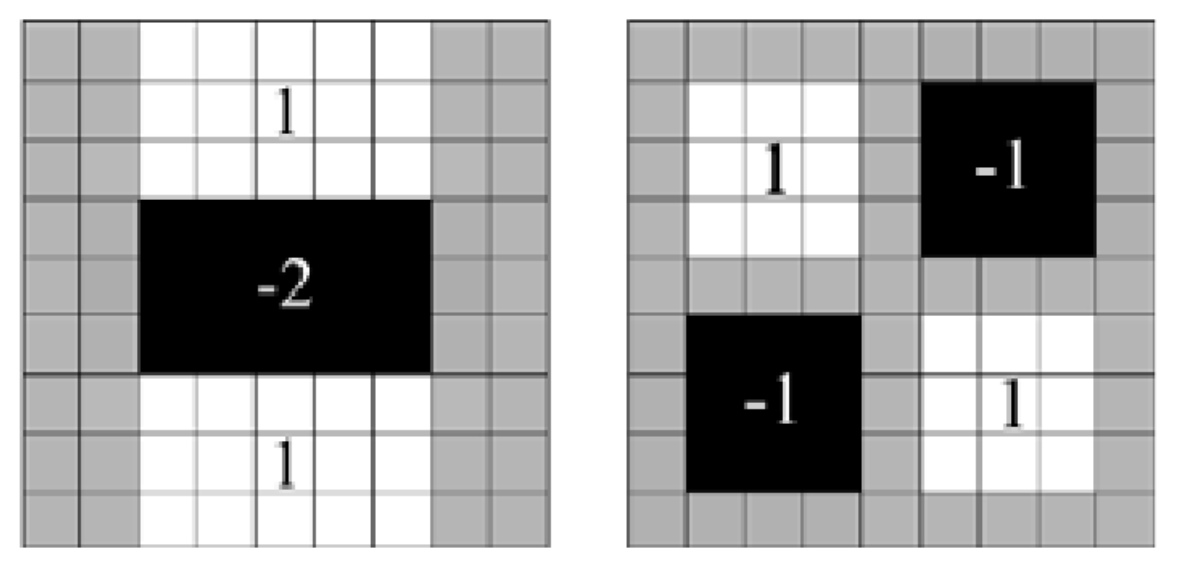
\includegraphics[width=0.5\textwidth]{./Images/SURF_BoxFilter.png}
    \caption{Box-Filter für zweite Ableitung nach y (links) und Ableitung nach xy (rechts). \cite{SURF}}
    \label{fig:surf:filter}
\end{figure}
Der Deskriptor wird in zwei Schritten berechnet. Zuerst wird die Hauptorientierung des Punktes berechnet. Dann wird auf dieser und der Skalierung basierend ein Bereich in dem Bild gewählt und in 16 Bereiche unterteilt.
Für jeden der 16 Bereiche wird die Intensität der Punkte in einem $4$ Bin großen Histogramm abgetragen, was zu einem Feature-Vektor der Größe $64$ führt.

BRIEF lässt die Frage der Wahl der korrespondierenden Punkt-Paare, die für den Intensitäts-Vergleich nötig sind offen, schlägt aber einige vor, wobei die zufällig generierten Paare die besten Ergebnisse liefern.
Ist die Wahl der Punkt-Paare abgeschlossen, kann der binäre Deskriptor gebildet werden. Dafür wird für jedes Paar die Differenz der Intensität zwischen den beiden Punkten ermittelt. 
Liegt die Differenz unter einem Schwellwert, wird die Position für das Paar im binären Deskriptor auf null gesetzt, ansonsten auf eins.
Vorteil an BRIEF ist, dass es weniger rechenaufwändig ist, verglichen mit SIFT, Nachteil an der Umsetzung ist, dass sie nicht rotationsinvariant ist.

ORB geht diesen Nachteil an, indem zuerst das Massezentrum des Bildes $C$ \ref{eq:sfm:orb:c} und dessen Orientierung $\theta$ \ref{eq:sfm:orb:theta} 
über die Momente $m_{00}$, $m_{10}$ und $m_{01}$ \ref{eq:sfm:orb:m} berechnet wird.
Mit diesen Parametern werden die Koordinaten der Paare umgeformt, um so der Anfälligkeit für Rotation entgegen zu wirken. 
Des Weiteren liefert ORB eine gelernte Paar-Auswahl von $256$ Paaren, die dahingehend optimiert ist, dass die Paare unkorreliert sind und eine hohe Varianz aufweisen.

\begin{equation}
    \label{eq:sfm:orb:m}
    m_{pq} = \sum_{x,y}{x^py^qI(x,y)}
\end{equation}
\begin{equation}
    \label{eq:sfm:orb:c}
    C = ( \frac{m_{10}}{m_{00}}, \frac{m_{01}}{m_{00}} )
\end{equation}

\begin{equation}
    \label{eq:sfm:orb:theta}
    \theta = atan2(m_{01},m_{10})
\end{equation}


Wurden die Features ermittelt, müssen korrespondierende Features zwischen den Bildern ermittelt werden. 
Hierzu muss die Distanz zwischen den Deskriptoren einzelner Features verglichen werden. 
Der korrespondierende Punkt des Feature-Punktes ist der mit der geringsten Distanz. 
Um falsche Paare zu vermeiden, können Paare unter einem gewissen Schwellwert ausgeschlossen werden und 
Paare, bei denen der nächstbeste korrespondierende Punkt eine sehr ähnliche Distanz aufweist. 
Das lässt darauf schließen, dass es sich um einen Feature-Punkt handelt, der sich in einem sich wiederholenden Muster befindet.
%Danach werden zwischen den Bildern Übereinstimmungen in den Featuren mittels RANSAC gesucht. 
%Gleichzeitig werden mittels RANSAC auch die einzelne Feature die keine Übereinstimmungen haben aus dem Verfahren ausgeschlossen.
Um aus den korrespondierenden Bildpaaren auf die Positionen der Kameras zu schließen, wird die Fundamental-Matrix $F=K_1^{-T}EK_2^{-1}$ für jedes Bildpaar ermittelt. 
$K_1$ und $K_2$ sind die beiden Kalibrierungs-Matrizen der Kameras und $E$ ist die Essential-Matrix, welche die Bewegung und Rotation der Kamera beschreibt.
Ist die Kalibrierung der Kamera bekannt, kann direkt $E$ berechnet werden.
$F$ beschreibt die Kamera-Bewegung und Rotation von einem zum anderen Bild, hat den Rang $2$ und bezieht dabei die Kalibrierung der Kameras mit ein.
%$E$ kodiert die Transformation bestehend aus der Rotation $R$ und der Translation $t$ zwischen den beiden Kamera-Positionen.
Um $F$ zu ermitteln werden mindestens acht korrespondierende Features $(p_{A1},p_{B1})...(p_{A8},p_{B8})$ zwischen den Bildern $A$ und $B$ eines Paares benötigt. 
Die Bildpunkte $p_{Ai}$ und $p_{Bi}$ der Paare sind dabei nicht in Pixel-Koordinaten angegeben sondern relativ zum Bild-Ebenen-Zentrum angegeben. 
Die Koordinaten liegen also in dem Bereich  $[-1, 1]$.
Da es sich um homogene Koordinaten handelt wird neben dem x und y Wert noch eine eins hinzugefügt.
Hierzu werden mindestens acht Gleichungen der Form $p_{Ai}^TEp_{Bi}=0$ gebildet und daraus ein Gleichungssystem der Form $Ax=0$ erzeugt, wobei $x$ die Unbekannten aus $F$ enthält.
Das Gleichungssystem wird mittels Singulärwertzerlegung (SVD) gelöst. Man erhält drei Matrizen $U$, $S$ und $V$. $U$ hat die Größe $m\times m$, $S$ die Größe $m\times 9$ und $V$ die Größe $9\times 9$.
$S$ ist eine Diagonal-Matrix deren Einträge die Singulärwerte in absteigender Reihenfolge enthält.
Aus der letzten Spalte von $V$, welche den kleinsten Singulär-Vektor enthält, kann die Approximation $\hat{F}$ von $F$ rekonstruiert werden. 
Wobei der Vektor der Länge $9$ zu einer Matrix der Größe $3\times3$ umgeformt wird.
Da durch Rauschen $\hat{F}$ den Rang $3$ haben kann, wird von $\hat{F}$ noch einmal die SVD gebildet und in $S$ das letzte Diagonal-Element explizit auf $0$ gesetzt, was hier als Matrix $\hat{S}$ beschrieben wird.
Damit kann die Approximation von $F$ neu berechnet werden ($\hat{F} = U\hat{S}V^T$) und hat damit Rang $2$.
Der Unterschied bei der Berechnung der Essential-Matrix ist, dass zum einen bei der Korrektur der Approximation neben dem letzten Eintrag der Diagonal-Elemente, das auf $0$ gesetzt wird, 
die beiden verbleibenden Diagonal-Elemente auf $1$ gesetzt werden. Die daraus resultierende Matrix wird im Folgenden mit $D$ bezeichnet. 
Des weiteren wird bei den homogenen Bildpunkten nicht $1$ gesetzt, sondern $c$, die Kamerakonstante.
%Zum anderen werden die Bildpunkte normiert.
%Der Bildmittelpunkt bildet dabei den Koordinaten-Ursprung und die Bildpunkte werden im Bereich von $-1$ bis $1$ angegeben.
Ist $E$ bekannt, kann die Kamera-Pose, bestehend aus dem Kamera Zentrum $c$ und der Kamera-Rotation $R$, geschätzt werden.
Hier ergeben sich vier mögliche Lösungen, die in Gleichung \ref{eq:sfm:camera:pose} zu sehen sind. Wobei $W=
\begin{bmatrix}
    0 & -1 & 0\\
    1 & 0 & 0\\
    0 & 0 & 1
\end{bmatrix}
$ ist.

\begin{equation}
    \label{eq:sfm:camera:pose}
    \begin{split}
    c_1=U(:,3),&\qquad R_1=UWV^T \\
    c_2=-U(:,3),&\qquad R_2=UWV^T \\
    c_3=U(:,3),&\qquad R_3=UW^TV^T \\
    c_4=-U(:,3),&\qquad R_4=UW^TV^T
    \end{split}
\end{equation}
Um zu überprüfen welche der vier Konfigurationen die richtige ist, kann geprüft werden ob die rekonstruierten 3D-Punkte vor beiden Kameras sind. Es wird die Konfiguration gewählt, bei der am meisten Punkte vor den Kameras sind.
Sind nun die ersten beiden Kamera-Posen bekannt, können weitere Kameras mittels Perspektive-n-Points-Algorithmus (PnP) hinzugefügt werden. 
Hierbei wird anhand der bereits ermittelten 3D-Punkte die Pose einer weiteren Kamera mittels Least-Square-Fit gefunden. Da die Pose der Kamera 6 Freiheitsgrade hat, werden mindesten 6 korrespondierende Punkte benötigt. 
Wurden alle Kamera-Posen und 3D-Punkte geschätzt, müssen diese noch einmal korrigiert werden. Diesen Schritt nennt man Bundle-Adjustment (BA).
Beim BA wird für jede der $m$ Kamera-Posen $A$ mit den Parametern $a_j$ jeder der $n$ 3D-Punkte $P_i$ der von der Kamera aufgenommen wurde zurück auf das Kamera-Bild projiziert und 
der Abstand des so ermittelten Bild-Punktes zum originalen Bild-Punkt aus der Feature-Detektion gemessen und minimiert. 
Das Optimierungsproblem kann, wie in Gleichung \ref{eq:sfm:bundle:adjustment} zu sehen, formuliert werden. 
\begin{equation}
    \label{eq:sfm:bundle:adjustment}
    \min_{a_j, P_i} = \sum_{i=1}^n \sum_{j=1}^m v_{ij} d(Q(a_j, P_i), x_{ij})
\end{equation}
Hierbei gilt $v_{ij} = 1$, wenn der Punkt $i$ von Kamera $j$ erfasst wurde und ansonsten $0$.
$Q(a_j, P_i)$ ist die geschätzte Projektion des Punktes $P_i$ auf das Bild der Kamera $j$ und $d(x,y)$ ist die Euklidische Distanz.

TODO: Explain $x_{ij}$

%Das Bild-Paar mit den meisten Übereinstimmungen wird als Basis für die Rekonstruktion der 3D-Punktwolke genutzt.
%Wurde aus den beiden Bildern eine initiale Punktwolke erstellt, wird diese mit den verbleibenden Bildern angereichert \cite{alouacheevaluation}. 

%Eine der bekanntesten Algorithmen ist SIFT \cite{Sift3D}.
%Einige Verfahren benötigen genaue Informationen über die Kamera Position, Ausrichtung und andere Angaben wie die Brennweite der Linse etc. 
%andere wiederrum lesen diese Informationen aus den EXIF-Headern der Bildern direkt aus, wenn diese zur Verfügung stehen, oder schätzen diese \cite{ODM} \cite{schoenberger2016mvs}.

Einige bekannte Implementationen von SfM sind Colmap \cite{schoenberger2016sfm},\cite{schoenberger2016mvs}, Open Drone Map (ODM) \cite{ODM}, OpenCV SfM-Pipeline \cite{opencv}, AliceVision (Meshroom)\cite{Moulon2012},\cite{Jancosek2011} und OpenMVG \cite{moulon2016openmvg}.

Colmap stellt eine Pipeline bereit, die eine inkrementelle Implementation von SfM anbietet. Initial wird nach korrespondierenden Bildern gesucht und diese dann inkrementell in die Rekonstruktion aufgenommen.
Colmap nutzt Root-SIFT als Feature-Detektor. Root-SIFT nutzt im Gegensatz zu normalen SIFT beim Feature-Matching nicht die Euklidische Distanz sondern die Hellinger-Distanz \cite{arandjelovic2012three}.

ODM stellt auch eine Pipeline bereit, die aus den Schritten SfM, Multi View Stereo und dem Ermitteln von Filterpunkten besteht. 
Eine Besonderheit bei ODM ist, dass es für jeden 3D-Punkt auch eine Normale liefert.

Meshroom, welches zur 3D-Rekonstruktion AliceVision nutzt, erstellt aus Basis von Bildern ein 3D-Modell. 
Hierzu wird nach der Erstellung der 3D-Punktwolke eine Triangulierung ermittelt um ein Mesh zu erstellen, welches danach texturiert wird.

OpenCV und OpenMVG stellen SfM-Pipelines zur Verfügung, wie sie in diesem Abschnitt beschrieben wurden. 
Bei der OpenCV-Implementierung muss - im Gegensatz zu den anderen Verfahren - die Kamerakonstante $c$ angegeben werden und wird nicht ermittelt.

TODO: OpenMVG separat beschreiben

Es wurden in den letzten Jahren große Fortschritte im Bereich tiefer Neuronaler Netze (Deep-Learning) \cite{lecun2015deep} zur Gewinnung von 3D-Punkwolken gemacht \cite{fan2016point} \cite{tatarchenko2017octree} \cite{wang2018pixel2mesh}. 
Mit diesen Verfahren ist es möglich, aus einer minimalen Datenbasis, die auch nur aus einem Bild bestehen kann, 3D-Punkwolken zu generieren.
Nachteil der Verfahren ist, dass auf dem Bild nur ein Objekt ohne Hintergrund abgebildet sein darf, oder dass das zu erkennende Objekt mit einer binären Maske maskiert werden muss.
Eine Rekonstruktion von komplexen Szenen ist so nicht oder nur mit sehr hohem Aufwand möglich \cite{rs11222644}. %und wird daher nicht weiter untersucht. 
%Der in \cite{rs11222644} vorgestellte Ansatz geht diese Problematik an und soll daher untersucht werden.

\subsection{Segmentierung von 3D-Punkwolken}
\label{sec:stand:segmentierung}

Unter der Segmentierung von 3D-Punktwolken versteht man, dass jedem Punkt ein Label zu zugewiesen wird, welches Auskunft über eine Eigenschaft des Punktes gibt.
Im Falle dieser Arbeit sollen Label wie Stamm, Blatt, Blüte oder Frucht vergeben werden.

Bei der Analyse von Pflanzen in Form von 3D Punktwolken gibt es einige nicht gelernte Lösungen \cite{ThreeBasics} \cite{ModelBased}, die das Segmentieren von 3D Punktwolken von Pflanzen in Stiele und Blätter behandeln. 
Diese Ansätze haben aber das Problem, dass sie nur unter bestimmten Bedingungen gute Ergebnisse liefern.

\cite{ThreeBasics} verfolgt den Ansatz, eine Punktwolke in Stamm und Blätter anhand der Hauptkrümmung um jeden Punkt zu segmentieren. 
Hierbei wird die Hauptkrümmung für einen Punkt so interpretiert, dass der Punkt als Stamm interpretiert wird wenn die Krümmung hoch ist. 
Es wird also davon ausgegangen, dass die Stämme eine höhere Krümmung aufweisen als die Blätter. 

In \cite{ModelBased} wird ein Ansatz verfolgt, der sich die zylindrische Form von Stielen zunutze macht, um diese von anderen Teilen der Pflanze, wie den Blättern, zu unterscheiden. 
Es wird das Model eines Zylinders in der Punktwolke gesucht und wird dieses gefunden, werden Punkte, die in das Model fallen, als Stamm klassifiziert.

Insbesondere die hohe Qualität der Punktwolken, die meist mit einem LIDAR-Scanner oder einem vergleichbaren Gerät erzielt wird, 
kann mit Bild basierten Methoden wie SfM nicht oder nur mit sehr großen Datenmengen und dem damit verbundenen Rechenaufwand erreicht werden. 
Ein weiteres Problem, welches viele Lösungen haben ist, dass der Hintergrund, also alles was nicht zur Pflanze gehört, manuell entfernt wird, 
oder der Hintergrund so vorbereitet wird, dass dieser beim erstellen der Punktwolke ignoriert wird und erst auf der freigestellten Pflanze der eigentliche Ansatz ausgeführt wird. 
Um diese Lösungen dennoch in einer voll automatischen Pipeline nutzen zu können, muss das Freistellen der Pflanzen erst automatisiert werden.

Auch im Bereich Segmentierung wurden große Fortschritte im Bereich Deep-Learning auf Punkwolken gemacht, die mit einer angelernten Netzarchitektur bestimmte Objekte erkennen und Teile davon segmentieren. 
Diese Ansätze können auch auf Pflanzen angewandt werden. Dazu müssen Architekturen wie PointNet\cite{qi2017pointnet}/PointNet++\cite{qi2017pointnet++} oder DGCNN \cite{dgcnn} auf Punktwolken von Pflanzen trainiert werden, 
da für diese Klasse von Objekten noch keine Gewichte trainiert wurden.

TODO: DGCNN auschreiben.

PointNet ermöglicht Segmentierung durch zwei Schritte. Erst wird ein globaler Feature-Vektor für die Punktwolke ermittelt und dann auf Basis dessen für jeden Punkt ein Feature-Vektor ermittelt.
Auf Basis dessen wird das Label bestimmt, dem der Punkt zugeordnet werden soll. 
Dabei wird jeder der $n$ Punkte der Punktwolke mit einer $3\times 3$ Matrix transformiert, deren Gewichte gelernt sind. Dieses Mininetz wird von den Autoren T-Net genannt.
Danach wird jeder Punkt nacheinander mittels eines Multi-Layer-Perceptron (MLP) mit zwei Layern, deren Ausgabe-Schicht jeweils die Größe $64$ hat, in einen neuen Feature-Raum überführt. 
Die Gewichte des MLP werden also über alle Punkte geteilt, was auch für die folgenden MLPs gilt. Der Feature-Vektor für einen Punkt besteht aus $64$ Elementen.
Die Punkte des Feature-Raums werden wieder mit einem T-Net, diesmal der Größe $64\times 64$, transformiert. 
Danach wird wieder ein MLP (drei Layer mit Ausgabeschichten der Größen $64$, $128$, $1024$) angewandt und mittels Max-Pooling der globaler Feature-Vektor der Größe $1024$ ermittelt. 
Dieser Vektor wird mit dem lokalen Feature-Vektor für jeden Punkt kombiniert und die daraus entstehende Matrix der Größe $n\times 1088$ wird mittels zweier MLP-Layer in eine Matrix der Größe $n\times m$ überführt, wobei $m$ die Anzahl der möglichen Label ist.
Der erste dieser MLPs hat drei Layer mit den Ausgangs-Schicht-Größen $512$, $256$ und $128$. Der Zweite besteht aus zwei Layern der Ausgangs-Schicht-Größen $128$ und $m$.
Die Architektur ist in Abbildung \ref{fig:point:net:arch} dargestellt.

\begin{figure}
    \centering
    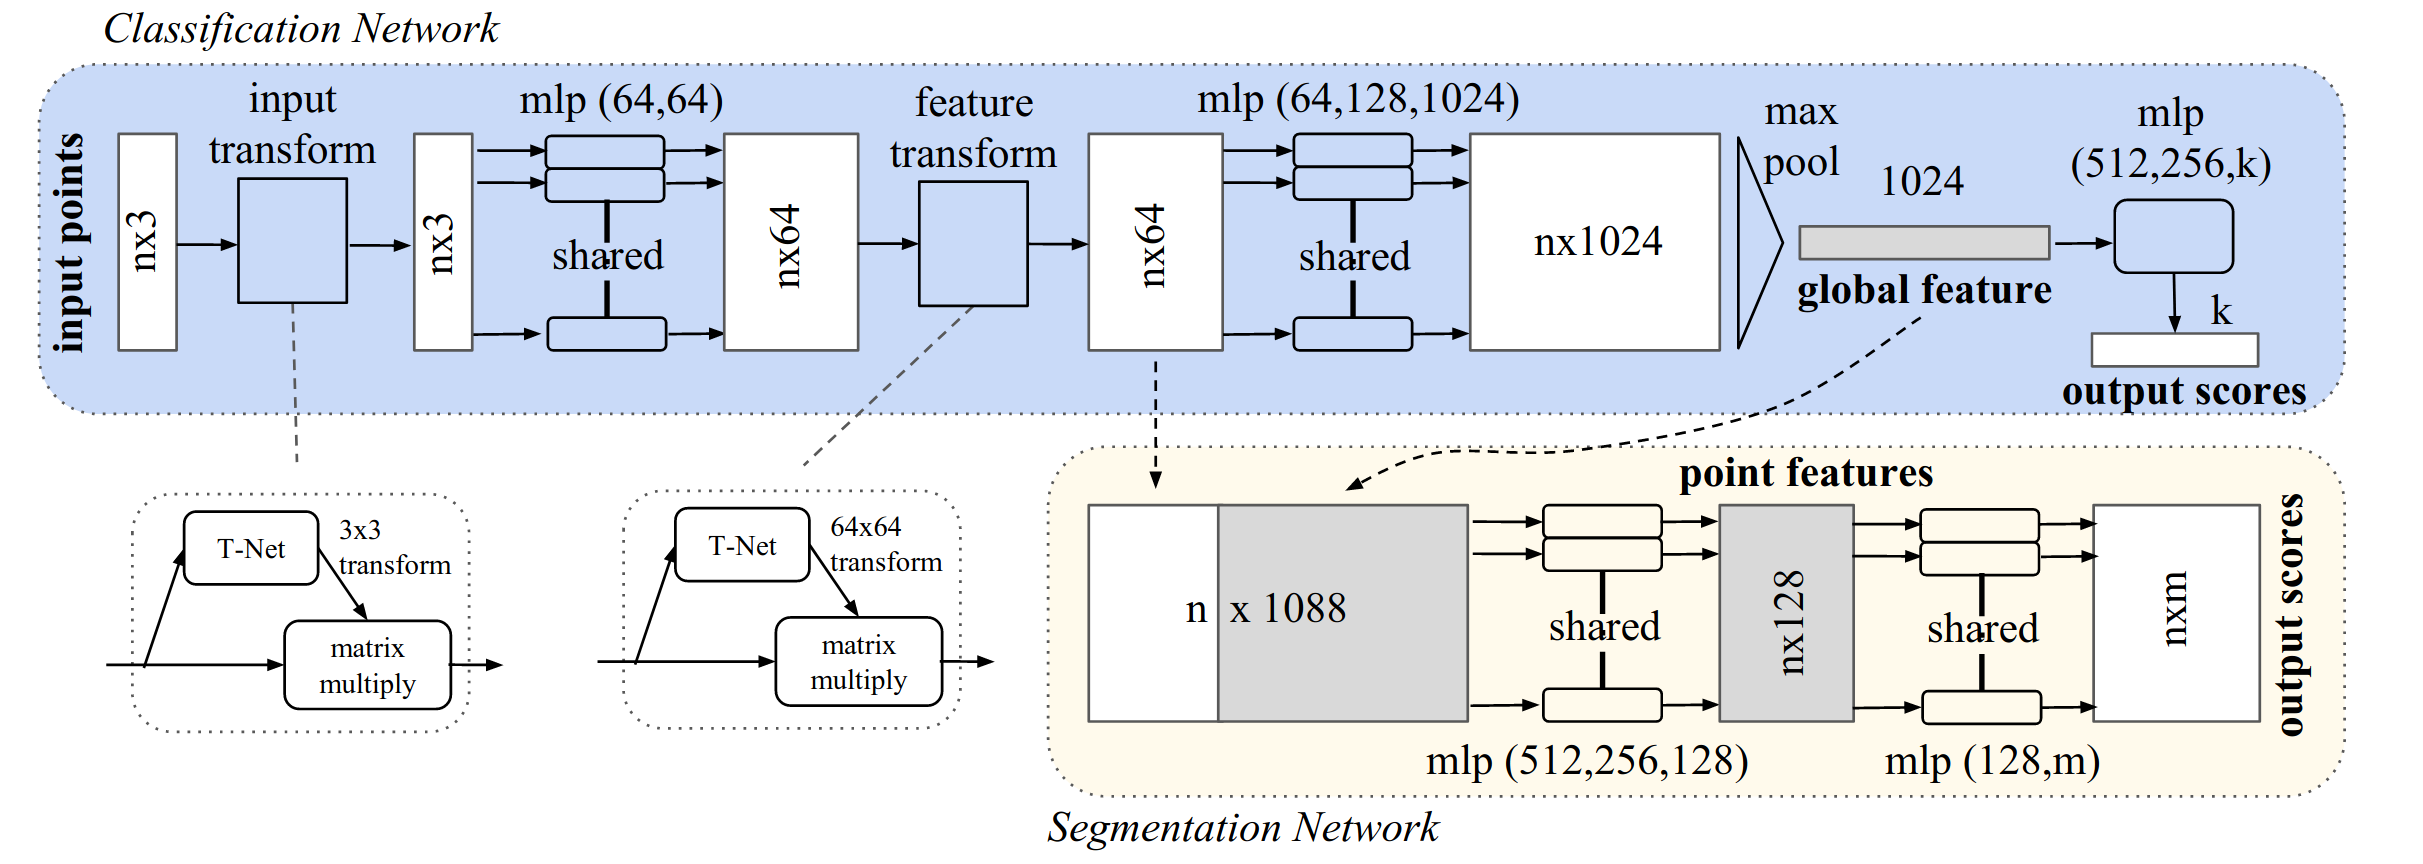
\includegraphics[width=1.0\textwidth]{./Images/PointNetArchitektur.png}
    \caption{PointNet-Architektur \cite{qi2017pointnet}}
    \label{fig:point:net:arch}
\end{figure}

PointNet++ baut auf der Architektur von PointNet auf. Hierbei wird das Problem adressiert, dass PointNet nicht gut mit kleinen Details umgehen kann. 
Um das zu bewerkstelligen werden kleinere Bereiche mit PointNet untersucht. Hier wird in drei Schritten vorgegangen: Sampling, Gruppieren und Feature-Vektor ermitteln.
PointNet++ führt also PointNet auf einem kleinen Bereich um gewählte zentrale Punkte aus. Beim Sampling werden diese zentralen Punkte mittels Farthest-Point-Sampling (FPS) ermittelt. 
FPS ermittelt aus $n$ Punkten eine Menge Punkte ${x_1,x_2,...,x_k}$, sodass der Punkt $x_j$ der Punkt mit dem weitesten Abstand zu allen Punkten der Menge ${x_1,x_2,...,x_{j-1}}$ ist.
Beim Gruppieren werden um die gewählten Punkte alle Punkte in den Bereich aufgenommen, die einen bestimmten Abstand $d$ von dem zentralen Punkt nicht überschreiten. 
Auf diesen Punkten wird PointNet angewandt. Für jeden zentralen Punkt wird also ein Feature-Vektor ermittelt.
Dieser Vorgang kann je nach Model mehrfach mit variierenden Parametern ausgeführt werden. 
Für die Klassifizierung wird nach dem letzten Layer auf dessen Ergebnis ein letztes mal PointNet angewandt, um den globalen Feature-Vektor zu ermitteln.
Bei der Segmentierung wird stattdessen, um jedem einzelnen Punkt ein Label zuzuordnen, der Prozess umgekehrt und mittels Interpolation werden die ermittelten Feature-Vektoren schrittweise auf die originalen Punkte 
übertragen. Dies geschieht unter Zuhilfenahme der in den vorherigen Schritten ermittelten Feature-Vektoren der zentralen Punkte.
Die vereinfacht dargestellte Architektur von PointNet++ ist in Abbildung \ref{fig:point:net:pp:arch} zu sehen.

\begin{figure}
    \centering
    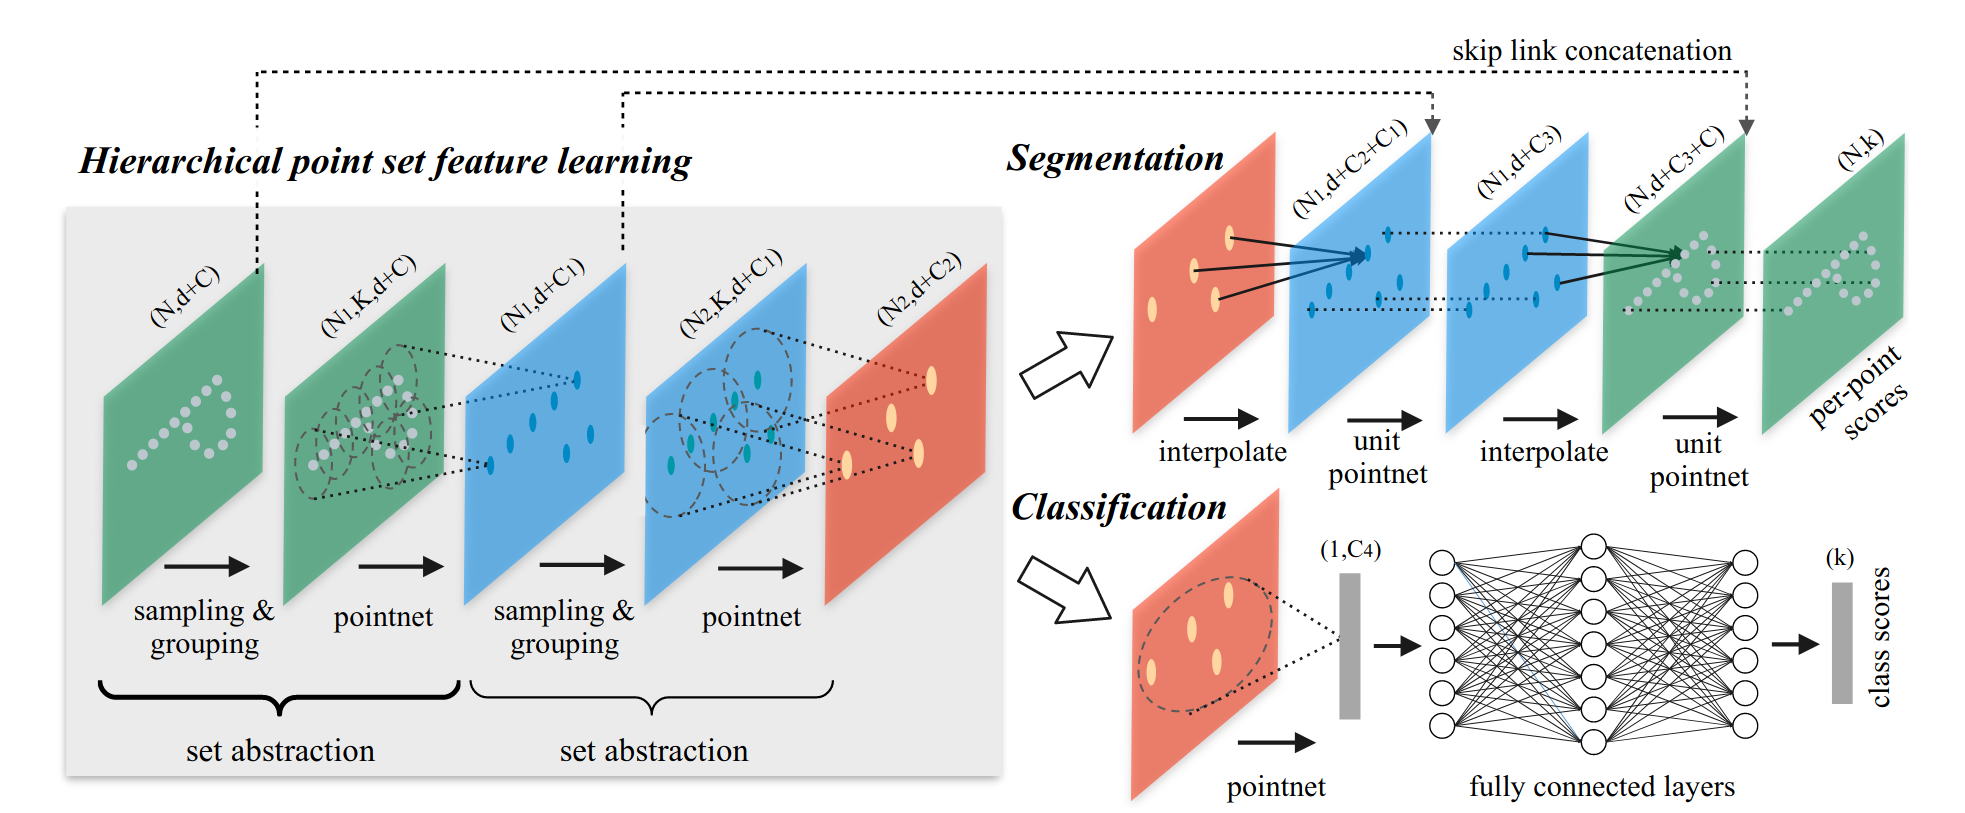
\includegraphics[width=1.0\textwidth]{./Images/PointNetPPArchitektur.png}
    \caption{PointNet++-Architektur \cite{qi2017pointnet++}}
    \label{fig:point:net:pp:arch}
\end{figure}

DGCNN führt Faltungen auf Nachbarschaftsgrafen der Punktwolke aus und ermittelt so für jeden Punkt einen Feature-Vektor. Die Nachbarschaftsgrafen werden mittels kNN gebildet.
Ähnlich wie bei PointNet wird erst der globale Feature-Vektor, der auch zur Klassifizierung genutzt wird, berechnet und dann darauf basierend die Feature-Vektoren für die einzelnen Punkte.
Ein weiterer Unterschied zu PointNet ist, dass die Ausgabeschichten vor dem Max-Pooling-Layer aggregiert werden.
Allerdings ist dir Güte von DGCNN bei Segmentierungs-Aufgaben, laut Angaben der Autoren \cite{dgcnn}, schlechter als die von PointNet++.

\subsection{Registrierung von 3D-Punkwolken}
\label{sec:stand:registrierung}

Bei der Registrierung von 3D-Punktwolken probiert man eine Transformationen $T$ zu finden, die eine Quell-Punktwolke $P_s$ so transformiert, dass der Abstand $d(P_s,P_t)$ zu einer Ziel-Punktwolke $P_t$ minimiert wird.
Das Abstandsmaß $d(P_s, P_t)$ kann verschieden formuliert werden. Eine Möglichkeit besteht darin die Summe über die Abstände eines jeden Punktes in $P_s$ 
zum nächsten Punkt in $P_t$ zu bilden und dies als Maß $d(P_s, P_t)$ zu nutzen. 

Die am weitesten verbreitete Methode zur Registrierung von 3D Punktwolken ist Iterative Closest Points (ICP) \cite{icp_org}. 
ICP basiert auf dem Ansatz, dass zwei Punktwolken iterativ aneinander angenähert werden, dies kann als Optimierungsproblem \ref{eq:icp} formuliert werden.
\begin{equation}
    \label{eq:icp}
    \underset{R,t}{\operatorname{argmin}}(\sum_{i=1}^N{\|Rp_{s_i} + t - p_{t_i}\|^2})
\end{equation}
Hierbei sind $R$ und $t$ die gesuchte Rotation und Translation und $p_{t_i}$ und $p_{s_i}$ bilden ein korrespondierendes Punktpaar aus den beiden zu registrierenden Punktwolken. 
$N$ ist die Anzahl Punkte in der Quell-Punktwolke.
ICP löst dieses Problem indem iterativ zwei Schritte durchgeführt werden. 
Erst werden die Zuordnungen für jeden Punkt in der Quell-Punktwolke zu einem Punkt in der Ziel-Punktwolke gesucht und danach die Rotation $R$ und Translation $t$ geschätzt, die die zugeordneten Punkte bestmöglich annähert.
Um eine Zuordnung zwischen den Punkten zu erreichen wird für jeden Punkt $p_i$ aus der Quell-Punktwolke $P_s$ der Punkt aus der Ziel-Punktwolke gesucht der $p_i$ am nächsten ist. 
%Bei der Bestimmung der Zurdnung gillt, je besser die Zurodnung der Punkte ist desto besser ist auch die Schätzung der Transformation.
Im zweiten Schritt wird zuerst für beide Punkwolken das Massezentrum $c_s$ und $c_t$ berechnet. Hierbei wird das Massezentrum $c$ einer Punktwolke $P$ mit $n$ Punkten, wie in \ref{eq:icp:mean} gezeigt, berechnet.
\begin{equation}
    \label{eq:icp:mean}
    c = \frac{1}{n}\sum_{i=1}^n{p(i)}
\end{equation}
Mit $c_s$ und $c_t$ lässt sich die Kreuzkovarianz-Matrix $H$ \ref{eq:icp:cross:cov} der beiden Punktwolken berechnen, auf der die SVD ($svd(H) = UDV^T$) angewandt wird.
\begin{equation}
    \label{eq:icp:cross:cov}
    H = \sum_{i=1}^n{(p_{t_i} - c_t)(p_{s_i} - c_s)^T}
\end{equation}
Sind $U$ und $V$ bekannt, kann damit die Rotation $R = VU^T$ und mit $R$ die Translation $t=c_t-Rc_s$ berechnet werden.
Da die Zuordnung im ersten Schritt nicht ideal sein muss wird der Vorgang solange wiederholt, bis es in der Transformation $T$, bestehend aus $R$ und $t$, zu keinen größeren Änderungen mehr kommt.
Das ist der Fall, wenn $T$ etwa der Einheitsmatrix entspricht.

Ein Problem das ICP hat ist, dass es auch für lokale Minima konvergiert. Das heißt, dass eine initiale Transformation für $P_s$ so gewählt werden muss, dass der ICP-Durchlauf bei einem globalen Minimum konvergiert.
Ansätze wie Go-ICP \cite{GoICP}, die mit verschiedenen initialen Transformationen starten, existieren, sind aber sehr rechenaufwändig und damit recht langsam.

Des weiteren ist ICP anfällig für Ausreißer. Für dieses Problem gibt es allerdings existierende Lösungen wie RICP \cite{ICP}. 
Hierbei kommt in der Regel RANSAC \cite{RANSAC} zum Einsatz, um Ausreißer bei der Registrierung auszuschließen.
RANSAC basiert auf der Idee, ein Modell in einer Punktwolke zu suchen und möglichst viele Punkte zu finden die in das Modell passen. 
Initial werden zufällig so viele Punkte wie nötig gezogen um das Modell minimal zu repräsentieren. 
So werden zum Beispiel für ein Linien-Modell zwei zufällige Punkte aus der Punktwolke gezogen. 
Nun werden die Parameter für das Modell mit den gezogenen Punkten ermittelt und alle Punkte, die nahe genug an dem so gebildeten Modell sind, mit aufgenommen.
Wenn der Anteil der Punkte die in das Modell fallen, über einem bestimmten Schwellwert liegen, terminiert der Algorithmus. 
Ansonsten wird der Vorgang solange wiederholt, bis eine Parametrisierung gefunden wurde, die terminiert oder eine Obergrenze an Iterationen erreicht wurde.
Das Ergebnis des Algorithmus ist auf der einen Seite die gefundene Parametrisierung. 
Auf der anderen Seite wird eine Unterteilung der Punkte in Punkte, 
die in das Modell fallen und in die, die nicht in das Modell fallen gefunden.
Letzteres kann genutzt werden um Punkte bei der Registrierung auszuschließen.

Ein weiteres Problem ist, dass die meisten ICP-Ansätze keine Werte für die Skalierung schätzen. 
Dies ist aber nötig, da bei SFM keine Information über die reale Ausdehnung eines Objektes ermittelt werden kann.
Es gibt einige wenige Ansätze für dieses Problem, die auch eine Schätzung für die Skalierung ermitteln \cite{Ziner2005PointSR}.
In \cite{Ziner2005PointSR} wird die Skalierung geschätzt, nachdem die Rotation $R$ bekannt ist, also nach der SVD. 
Ist $R$ bekannt, können die Vektoren $s$ und $t$ gebildet werden (Siehe Gleichung \ref{eq:icp_scale:1}).

\begin{equation}
    \label{eq:icp_scale:1}
    s_i = R (p_{s_i} - \bar{p_s}),\quad t_j = p_{t_j} - \bar{p_t}
\end{equation}

Mittels dieser Vektoren kann die Skalierung $scale$ berechnet werden. Die Berechnung ist in Gleichung \ref{eq:icp_scale:2} zu sehen.

\begin{equation}
    \label{eq:icp_scale:2}
    scale = \sum_{i,j}{t_j^Ts_i} / \sum_{i}{s_i^Ts_i}
\end{equation}

Auch für das Registrierungs-Problem gibt es Lösungen aus dem Deep-Learning-Bereich. Aber auch hier gibt es das Problem, dass es nur wenige Ansätze gibt, die mit Skalierung umgehen können \cite{ScaleLK}.
Bekannte Ansätze sind DCP \cite{Wang_2019_ICCV}, PointNetLK \cite{aoki2019pointnetlk} und RPM-Net \cite{Yew_2020}.
%DeepGMR \cite{yuan2020deepgmr}, PRNet \cite{wang2019prnet} und PCRNet \cite{sarode2019pcrnet}.
Diese Ansätze sollen in dieser Arbeit untersucht werden.

DCP besteht aus drei Teilen. Wobei es sich bei den ersten zwei Teilen um Netze handelt, die eine Zuordnung berechnen die der von ICP ähnelt, aber mehrere Zurodnungen für einen Punkt nutzt und diese gewichtet.
Das erste Netz berechnet für jeden Punkt einen Feature-Vektor. Hier wurde von den Autoren PointNet und DGCNN untersucht, wobei DGCNN die besseren Ergebnisse liefert. 
Das zweite Netz kodiert den Feature-Vektor mittels eines Transformer-Modells weiter. 
Transformer-Modelle wurden ursprünglich entwickelt um kontextuelle Information von Sätzen zu kodieren und dekodieren um so Aufgaben wie Übersetzung von Sprachen zu ermöglichen. 
Dieses Prinzip wird hier auf die Registrierung übertragen, wobei hier eine Zurodnung zwischen den beiden Punktwolken gesucht wird.
Bei der so gefundenen Zuordnung handelt es sich um eine weiche Zuordnung. Das heißt ein Punkt in der Quell-Punktwolke kann nicht nur einem sondern mehren Punkten in der Ziel-Punktwolke zugordnet werden.
Der letzte Teil von DCP schätzt auf Basis dieser Zuordnung wie bei ICP mittels SVD Rotation und Translation, die für die Registrierung nötig sind.
Auch bei DCP wird der Prozess bis zur Konvergenz des Registrierungs-Ergebnisses wiederholt.

PointNetLK basiert auf der Idee von PointNet und dem LK-Algorithmus \cite{lk} der zur Registrierung von Bildern entwickelt wurde und mit dem sich der optische Fluss von einem zum anderen Bild beschreiben lässt. 
Hierbei wird PointNet für die Ziel und Quell-Wolke ausgeführt und die Distanz zwischen den globalen Feature-Vektoren minimiert und 
dabei eine Transformation $G$ gefunden die den Abstand zwischen Ziel- und Quell-Punktwolke minimiert.
Der Vorgang wird wiederholt, bis die Distanz der Feature-Vektoren unter einem gewissen Schwellwert liegt, bzw die Transformation $G$ der Einheitsmatrix ähnelt.
Über die Iterationen müssen sich die berechneten Transformationen gemerkt und zum Schluss miteinander multipliziert werden um die finale Transformation zu finden, die die beiden Punktwolken miteinander registriert.

%Initial wird die Ziel-Punktwolke der Größe $n\times 3$ in einen hochdimensionalen Vektorraum der Größe $n\times k$ mittels eines MLP überführt. 
%Aus der Ausgabe des MLP-Layers wird mittels einer symmetrischen Polling-Funktion ein $k$ großer globaler Feature-Vektor ermittelt. Für diesen wird die Jakobi-Matrix $J$ berechnet.
%Die Quell-Punktwolke wird nun iterativ an die Ziel-Punktwolke angenähert.
%Die Quell-Punktwolke wird dabei ähnlich wie die Ziel-Punktwolke behandelt. Es wird allerdings nach dem ermitteln des globalen Feature-Vektors nicht die Jakobi-Matrix gebildet, 
%sondern mittels der Moore-Penrose Inversen Matrix von $J$ und der Differenz der beiden globalen Feature-Vektoren die Parameter für die in dieser Iteration auszuführenden Transformation ermittelt.
%Die Transformation wird angewandt und der Vorgang solange wiederholt bis es zu keinen oder nur noch kleinen unter einem Schwellwert liegenden Änderungen in den Parametern für die Transformation kommt.
%Die einzelnen Transformationen aus den Iterationen werden miteinander multipliziert um die Transformation zu erlangen die die Quell-Punktwolke mit der Ziel-Punkwolke registriert.

RPM-Net baut auf RPM \cite{RPM} auf. RPM hat zu ICP den Unterschied das zwischen den Punkten beider Punkwolken auch die Zuordnung der Punkte mit in das Optimisierungsproblem einfliest.
Damit wird das Optimierungs-Problem \ref{eq:icp} umformuliert zu \ref{eq:rpm:opt}.
\begin{equation}
    \label{eq:rpm:opt}
    \underset{M,R,t}{\operatorname{argmin}}(\sum_{i=1}^N\sum_{k=1}^K{m_{jk}(\|Rp_{s_i} + t - p_{t_k}\|_2^2-\alpha)})
\end{equation}
Dabei ist $M$ die Gewichtungsmatrix für die Zuordnungen zwischen den Quell und Zielpunkten und der Parameter $\alpha$ ist dazu da um Korrespondenzen zwischen Paaren auszuschließen. 
Die Idee dabei ist, das Distanzen unter dem Schwellwert $\alpha$ die Kosten senken.
Die Matrix $M$ wird in jeder Iteration wie in \ref{eq:rpm:m} initialisiert.
\begin{equation}
    \label{eq:rpm:m}
    m_{ij} = e^{-\beta(\|Rp_{s_i} + t - p_{t_j}\|_2^2-\alpha)}
\end{equation}
Dabei ist $\beta$ ein Parameter der über die Itarationen erhöht wird.

Im Vergleich zu RPM werden die räumlichen Entfernung bei der Berechnung von $M$ durch hybride Feature-Distanzen ersetzt \ref{eq:rpm:net:m}.
\begin{equation}
    \label{eq:rpm:net:m}
    m_{ij} = e^{-\beta(\|\hat{f}_{s_i} - f_{t_j}\|_2^2-\alpha)}
\end{equation}
Wobei $\hat{f}_{s_i}$ der hybride Feature-Vektor für den aus der vorherigen Iteration transformierten Punkt $p_{s_i}$ ist und $f_{t_j}$ der Feature-Vektor für den Punkt $p_{t_j}$
Des weiteren werden die Parameter $\alpha$ und $\beta$ in jeder Iteration durch ein neuronales Netz geschätzt. 
$\beta$ wird dabei nicht wie in RPM immer weiter erhöht, sondern basierend auf der Eingabe geschätzt.
Zuletzt wird wie beim ICP die SVD der Punktpaare ermittelt und so die Rotation gefunden, nur fließt beim Bilden der SVD auch das Gewicht der einzelnen Paare mit ein. 
Die Transformation kann so wie bei ICP ermittelt werden. 

%$\alpha$ ist ein Parameter der bei der Korrespondenz-Suche steuert welches Punkt-Paar mit einbezogen wird.
%$\beta$ steuert die härte der Zuordnung und wird iterativ erhöht.
 Details der Architektur sind in Abbildung \ref{fig:rpm:net:arch} zu finden.

\begin{figure}
    \centering
    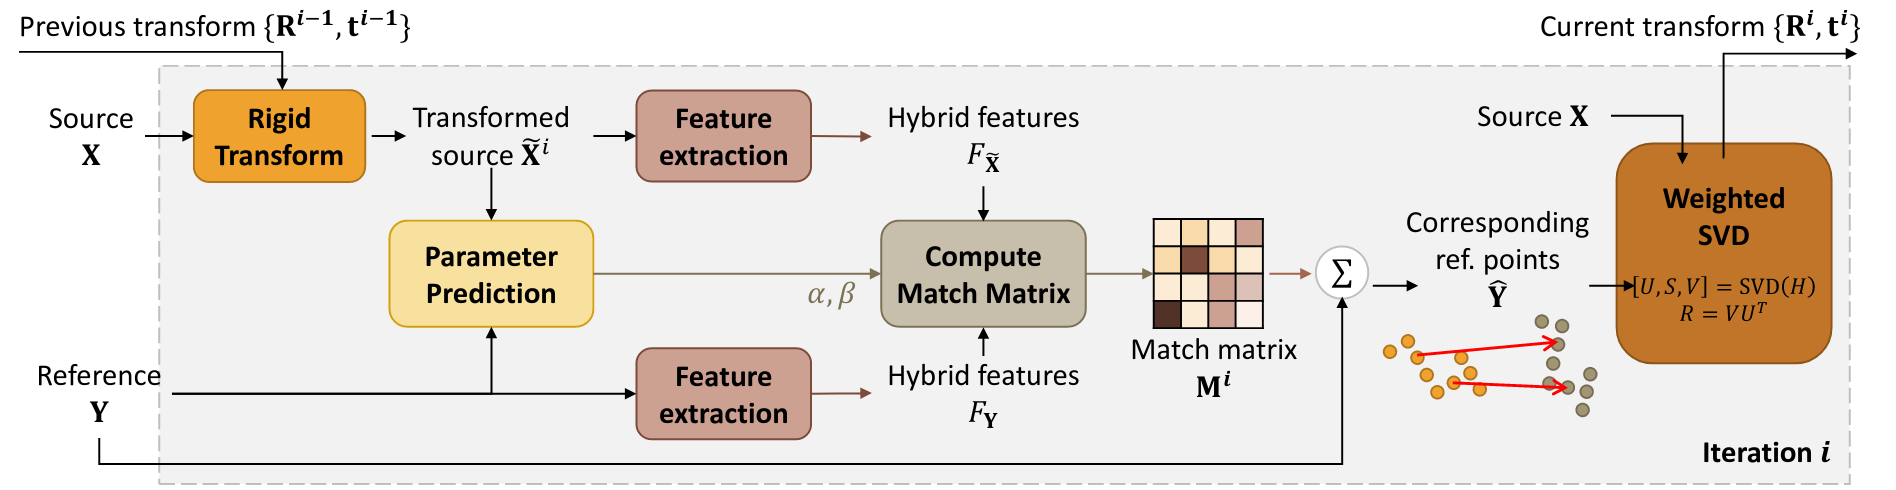
\includegraphics[width=1.0\textwidth]{./Images/RPM_Net_Arch.png}
    \caption{RPM-Net-Architektur \cite{Yew_2020}}
    \label{fig:rpm:net:arch}
\end{figure}

\newpage
\section{Realisierung}
%-------------------------------------------------------------
\label{sec:realisierung}
Es müssen vier Teilprobleme berücksichtigt werden. Zu Beginn muss aus einer Reihe von Bildern einer Pflanze aus verschiedenen Perspektiven eine Punktwolke generiert werden. 
Hauptziel hierbei ist es, möglichst wenig Bilder zu benötigen. 
Trotzdem müssen Aspekte wie die Qualität der Punkwolken berücksichtigt werden. Diese sollten die aufgenommene Szenen klar darstellen und wenig Rauschen und andere Störungen enthalten. 
Bei der Aufnahem sollte darauf geachtet werden, dass zwischen den aufeinander folgenden Bildern immer mindestens 50\% Überschneidung, in der zu sehenden Szene, sichergestellt ist. 

Ein zweites Problem ist die Registrierung zweier Punktwolken einer Pflanze zu verschiedenen Zeitpunkten um diese vergleichen zu können. 
Hierbei gilt es, die ideale Transformation $T$, bestehend aus Rotation, Skalierung und Translation zu finden, um die beiden Punktwolken so realitätsnah wie möglich aneinander aus zu richten.
Es werden drei Ansätze überprüft, dieses Problem zu lösen. 
Allen Ansätzen liegt zugrunde, dass beim Beginn einer neuen Zeitserie zur Analyse eines Wachstumsprozesses, eine Punktwolke des Hintergrunds erstellt wird und 
die Punktwolken der einzelnen Zeitpunkte mit diesem Hintegrund zu registrieren. So wird ein Verhältnis geschaffen, das dem der Realität entspricht. 
Wird für einen beliebigen Zeitpunkt noch die totale Größe der Pflanze angegeben, kann aus den Verhältnissen die totale Größe aller Zeitpunkte berechnet werden. 
Der erste Ansatz soll dabei untersuchen ob es mit einer angepassten Version von ICP möglich ist, neben der Rotation und Transformation auch die relative Skalierung zur Hintergrund-Punkwolke zu ermitteln.
Der zweite Ansatz soll untersuchen, ob DCP so angepasst werden kann, dass statt Rotation und Translation separat, die komplette Transformations-Matrix mit Skalierung geschätzt werden kann.
In einem letzten Ansatz soll die Skalierung durch iteratives Anwenden verschiedener Skalierungen gefunden werden, mit einer anschließenden Registrierung ohne Schätzung der Skalierung.

Das dritte Problem ist die Segmentierung der Punktwolke in Stamm, Blätter und Hintergrund. Hier gibt es viele Ansätze, dieses Problem zu lösen. Allerdings ist es schwer, eine allgemein gültige Lösung zu finden. 
Ziel ist es daher eine Lösung zu finden die auf möglichst vielen Varianten von Pflanzen funktioniert. 
Das Problem der Segmentierung ist essentiell für die weitere Analyse einer Zeitserie. 
Ohne die Information welche Punkte zu Stamm und Blättern gehören kann nicht auf die Entwicklung von Blättern und Stielen im Einzelnen geschlossen werden.

Zuletzt müssen die Implementationen der Probleme in geeigneten Pipelines zusammengefasst werden und durch einen Server angesteuert werden. Hier muss die Lastverteilung und Datenhaltung beachtet werden.

\subsection{Architektur}
%-------------------------------------------------------------
\label{sec:realisierung:architektur}
%Zwingend erforderlich ist ein Überblick über die Komponenten Ihrer Lösung
%und deren Zusammenspiel. Dazu gehört in der Regel auch ein Diagramm
%der Systemarchitektur.

Die Anwendung soll über eine REST-API angesteuert werden können. Mit dieser soll es möglich sein neue Messreihen anzulegen. Dazu müssen die Bilder für die initiale Punkwolke auf den Server übertragen werden. 
Es soll ebenfalls möglich sein, weitere Messpunkte zu einer Messreihe hinzuzufügen. Zu einer Messreihe sollen Auswertungen zur Verfügung gestellt werden. 
Da in den einzelenen Teilaufgaben mit Laufzeiten die Länger als 10 Sekunden sind zu rechnen ist, sollen die Pipelines in einzelnen Jobs unterteilt werden und diese asynchron im Hintergrund abgearbeitet werden.
Dadurch reagiert die Anwendung schneller und bei größerer Last können einzelnen Verbindungen zu den Clients schnell wieder geschlossen werden. 
Um trotzdem Auskunft über den aktuellen Bearbeitungs-Status einer Pipeline geben zu können, soll dieser durch eine weitere Schnittstelle abrufbar sein und Auskunft über den Status der einzelenen Jobs geben.
%Zu jeder Messreihe soll ein Bearbeitungs-Status abgerufen werden können, da die einzelnen Aufgaben asynchron im Hintergrund ausgeführt werden sollen.

Die einzelnen Abläufe sind in Abbildung \ref{fig:WorkflowClientServer} zu sehen.

\begin{figure}
    \centering
    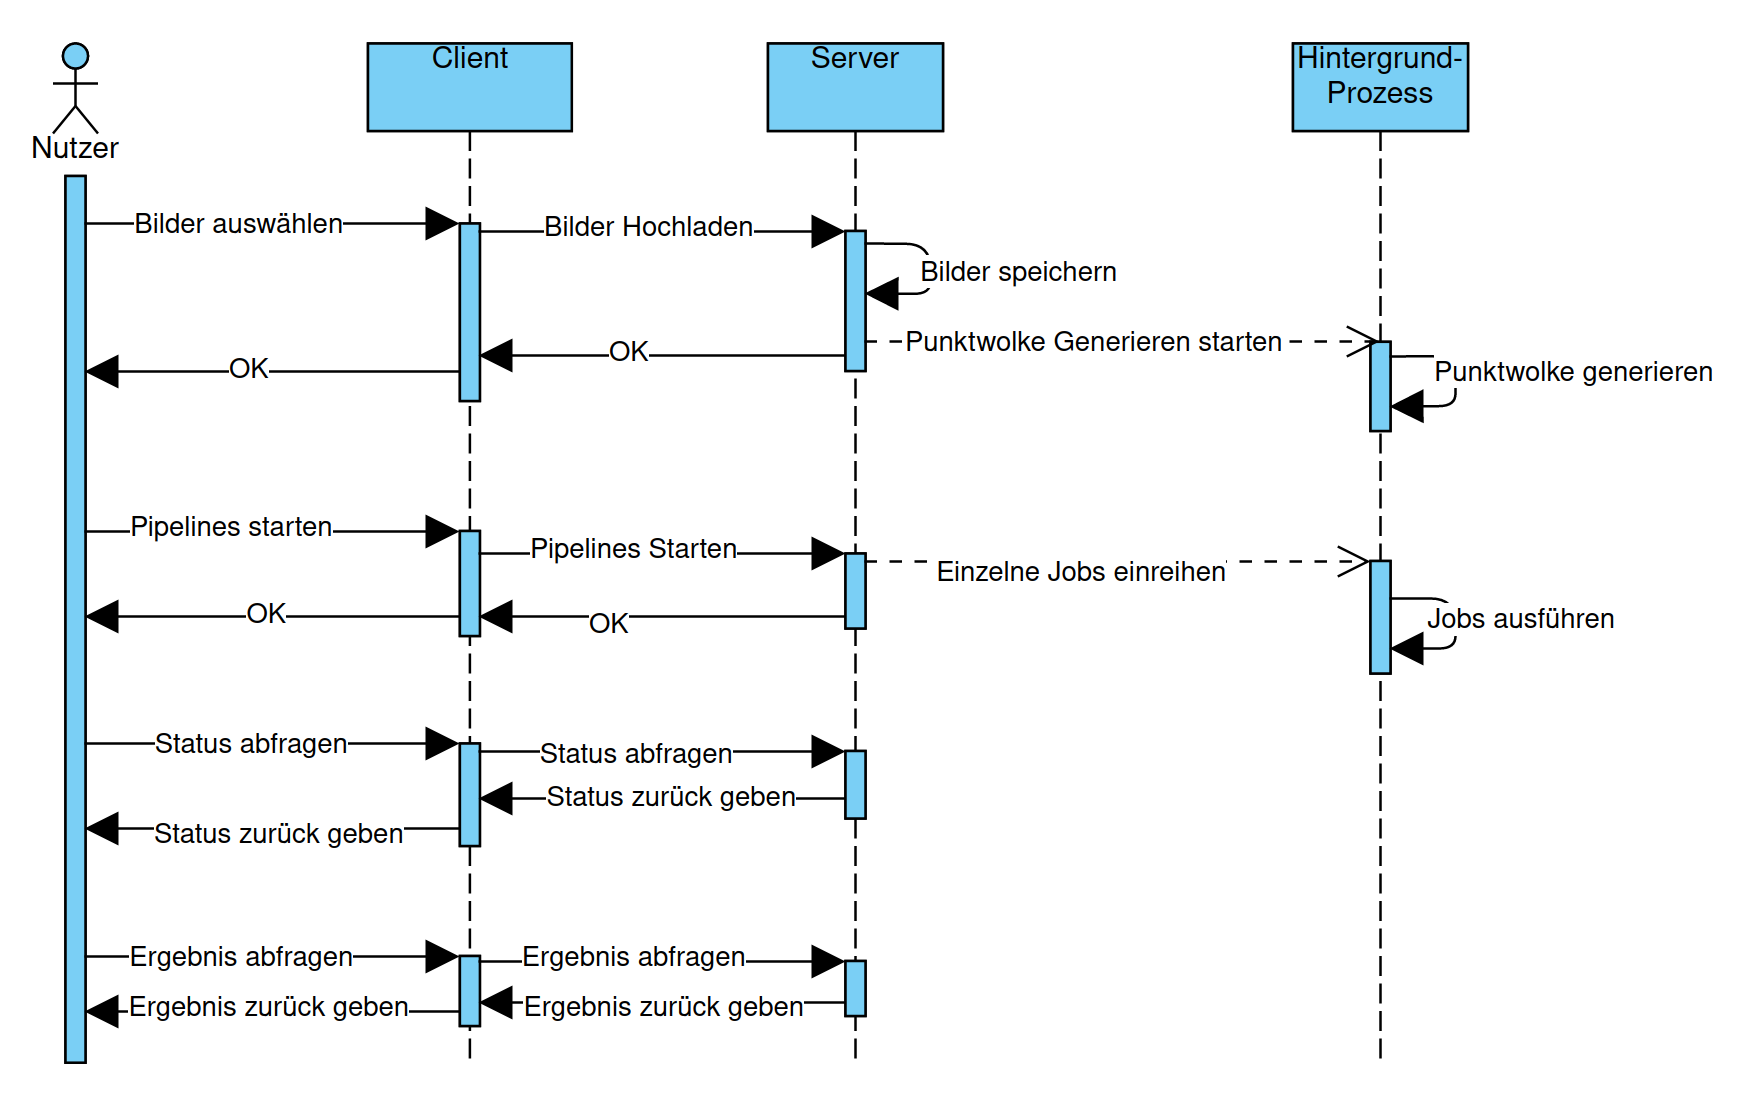
\includegraphics[width=0.9\textwidth]{./Images/WorkflowClientServer.png}
    \caption{Arbeitsabläufe zwischen Nutzer, Client, Server und Hintergrundprozess.}
    \label{fig:WorkflowClientServer}
\end{figure}

\subsection{Umsetzung Generierung einer 3D Punktwolke aus Bildern}
%-------------------------------------------------------------
\label{sec:realisierung:implementierung1}
%Dies ist in der Regel nicht nur ein Abschnitt, sondern mehrere Abschnitte
%mit Ihrem Projekt angemessenen Überschriften. Hierhin gehört {\em nicht}
%der Sourcecode Ihrer Lösung, sondern eine textuelle und grafische
%(z.B.~Klassendiagramm) Beschreibung. Bei Quellcode beschränken Sie Sich
%bitte auf kurze, aussagekräftige Ausschnitte.

Die aus der Analyse der verschiedenen Verfahren (siehe Evaluation) ausgewählte Anwendung ODM wird als Docker bereit gestellt. Um den Docker erfolgreich auszuführen, muss eine Ordner bereit gestellt werden.
In diesem Ordner muss ein Ordner \glqq images\grqq{} enthalten sein, der die Bilder des Datensatzes, aus dem eine Punktwolke generiert werden soll, enthält.

Ist das Verzeichnis angelegt, kann der Docker gestartet werden. Hierbei muss allerdings beachtet werden, dass der Docker mit denselben Rechten wie der User ausgeführt wird. 
Ansonsten werden per Standarteinstellung Root-Rechte genutzt.
Das führt dazu, dass auf die erstellten Daten nur noch lesend zugegriffen werden kann, was das Aufräumen nur mit Root-Rechten ermöglicht.
Nach dem Ausführen des Dockers sollten in jedem Fall alle nicht benötigten Dateien gelöscht werden, da diese je nach Anzahl genutzter Bilder mehrere Gigabyte an Festplattenspeicher belegen.

\subsection{Umsetzung Registrierung zweier Punktwolken}
%-------------------------------------------------------------
\label{sec:realisierung:implementierung2}

Bei der Umsetzung der Registrierung muss die Besonderheit beachtet werden, dass die Skalierungen der Punktwolken nicht bekannt sind und sich unterscheiden. 
Das heißt die Punkwolken liegen in unterschiedlichen Maaßtäben vor.  
Um ein gutes Verfahren zu finden, was mit dieser Besonderheit umgehen kann, werden mehrere Ansätze verglichen.

In einem ersten Ansatz wird versucht, eine Pipeline, auf Basis von ICP, zu erstellen, die eine gute initiale Lösung findet ohne den ganzen möglichen Suchraum zu durchsuchen.
Die Pipeline sucht zuerst für die Quell- und Ziel-Punktwolke $S$ und $T$ nach der größten Ebene in der Punkwolke und richtet die Punkwolke so aus, dass die gefundene Ebene auf der Ebene liegt, die die x und y Achse bilden.
Zudem werden die Punkwolken so skaliert, dass die begrenzenden Boxen gleich groß sind.
Des weiteren werden aus beiden Punkwolken nur eine Teilmenge $P_c$ der Punkte in einem Radius $r$ um den Punkt $c$, der das Zentrum der Masse der Punktwolken repräsentiert, entnommen.
Damit soll Rauschen und unvollständige Fragmente an den Rändern unterdrückt werden und ein Teil des Hintergrunds soll ausgeblendet werden.
Aus dieser Teilmenge werden Subsample gezogen um den Rechenaufwand zu minimieren. In diesem Zustand haben Quell- und Ziel-Punktwolke eine gute initiale Transformation.
Für die zu registrierende Punktwolke wird zunächst mittels SIFT 3D \cite{Sift3D} eine Verbesserung der initialen Transformation gesucht. 
Danach wird ein ICP-Durchlauf gestartet, der auch die Skalierung der Ziel-Punktwolke schätzt.
Um das Ergebnis nach der Schätzung der Skalierung weiter zu verbessern, wird erneut ein ICP-Durchlauf gestartet - diesmal ohne Schätzung der Skalierung.

Ein weiterer Ansatz ist es, DCP so abzuwandeln, dass statt Translations-Vektor und Rotations-Matrix direkt die ganze Transformations-Matrix geschätzt wird. 
Dazu muss der SVD-Head so angepasst werden, dass statt einer $3\times 3$ Rotations-Matrix $R$ und dem Translations-Vektor $\vec(t)$ die Translations-Matrix $T$ zurück geliefert wird.
Um das zu erreichen muss die Eingabe der Größe $N\times 3$ auf eine Eingabe der Größe $N\times 4$ erweitert werden. Hier kann die Eingabe um einen Vektor mit Einsen erweitert werden.
Das führt dazu das die SVD von $H$ im SVD-Head nun eine $4\times 4$ Matrix ist. Wir nehmen an, dass die SVD $H$ als Transformations-Matrix interpretiert werden kann.

In einem letzten Ansatz wird die Skalierung geschätzt, indem ein vorgegebener Bereich an Werten für die Skalierung in einer vorgegebenen Schrittgröße $s$ dursucht wird.
Wieder werden Quell- und Ziel-Punktwolke an der XY-Ebene ausgerichtet und eine Teilmenge $P_c$ um das Zentrum $c$ entnommen, wie im ersten Ansatz. Auch werden wieder Subsample gezogen.
In jedem Skalierungs-Schritt wird die Punktwolke mit der aktuellen Skalierung skaliert und danach mit einem Registrierungs-Verfahren registriert.
Um die Ergebnisse der einzelnen Registrierungen zu messen, wird der Abstand zwischen der transformierten Quell-Punktwolke und der Ziel-Punktwolke berechnet. 
Der Abstand $d(S,T)$ wird so berechnet, dass für jeden Punkt $p$ aus der Punktwolke $T$ der Abstand zum nächsten Punkt in der Punktwolke $S$ berechnet wird.

Man könnte auch den Abstand von allen Punkten in $S$ messen, aber das kann zu Problemen bei kleinen Skalierungen führen, 
da im Extremfall einer sehr kleinen Punktwolke $S$ alle Punkte in $S$ nahezu keinen Abstand mehr zueinander haben.
Man könnt $S$ also auch durch einen Punkt $p_{S}$ abstrahieren.
Bei der Registrierung muss $S$ nur sehr nah an einem Punkt $p_t$ in $T$ sein, sodass gilt $p_t \approx p_S$ und der Abstand zwischen $S$ und $T$ geht gegen $0$. 
Dadurch werden sehr kleine Skalierungen durch dieses Maß bevorzugt.
Nimmt man statt aller Punkte in $S$ alle Punkte in $T$, wird der Fehler in diesem Fall größer als $0$ sein, es sei den $T$ ist auch sehr klein.

Mit diesem Maß kann man nun die Güte der einzelnen Skalierungs-Iterationen bewerten und die beste Skalierung mit zugehöriger Transformation für Rotation und Translation finden.
Da die Wahl des Registrierungs-Verfahren offen bleibt wurden hier mehrere Verfahren miteinander verglichen. Es wurden neben zwei ICP-Implementationen DCP, PointNetLK und RPM-Net miteinander verglichen.

\subsection{Umsetzung Segmentierung}
%-------------------------------------------------------------
\label{sec:realisierung:implementierung3}

Zur Segmentierung der Pflanzen-Punktwolke in Stamm und Blätter wurde ein Ansatz verfolgt, der an den in \cite{ThreeBasics} angelehnt ist.
In \cite{ThreeBasics} wird mittels der Hauptkrümmung eines Punktes ermittelt, ob es sich bei dem Punk um ein Blatt oder einen Stiel handelt. 
Hierbei wird eine einfache Entscheidungsregel $f(x)$ mittels eines Schwellwerts $T_k$ genutzt: 
Ist die Stärke der Krümmung $k(x)$ des Punktes höher als der Schwellwert, handelt es sich um einen Stiel, da diese eine größere Krümmung haben als Blätter.
Die Schwierigkeit besteht darin einen guten Schwellwert und eine gute Kennzahl für die Stärke der Krümmung zu finden.

Die Hauptkrümmung eines Punktes $p_i$ kann über die Normalen des Punktes und der $k$ nächsten Nachbarpunkte $P_i$ berechnet werden.

\begin{equation}
\label{eq:hauptkruemmung:1}
\vec{m}_j = (I - \vec{n}_i \otimes \vec{n}_i ) \cdot \vec{n}_j
\end{equation}

Aus den Abbildungen $\vec{m}_j$ (siehe Gleichung \ref{eq:hauptkruemmung:1}) für alle $P_i$ kann die Kovarianzmatrix $C_i$ berechnet werden, wie in Gleichung \ref{eq:hauptkruemmung:2} zu sehen ist.

\begin{equation}
\label{eq:hauptkruemmung:2}
C_i = \frac{1}{k} \sum_{j=1}^k{(\vec{m}_j - \vec{\bar{m}}) \otimes (\vec{m}_j - \vec{\bar{m}})}
\end{equation}

Die Hauptkrümmung kann aus den Eigenwerten $0 \leq \lambda_1 \leq \lambda_2 \leq \lambda_3$ von $C_i$ bestimmt werden. $\lambda_3$ ist die stärkste Krümmung und $\lambda_2$ die schwächste Krümmung.

In \ref{eq:hauptkruemmung:3} sind einige der untersuchten Ansätze für eine Funktion $k(p_i)$ zu finden. 

\begin{equation}
\label{eq:hauptkruemmung:3}
\begin{array}{ll}
k_1(p_i) = \lambda_3 \\
k_2(p_i) = \lambda_2 \\
k_3(p_i) = (\lambda_3 + \lambda_2) / 2 
\end{array}{}
\end{equation}

Je höher der Wert der Funktion $k(p_i)$ aus den Gleichungen in \ref{eq:hauptkruemmung:3} ist, desto wahrscheinlicher gehört ein Punkt zum Stiel einer Pflanze. 
Die Entscheidungregel dafür zeigt Gleichung \ref{eq:manuell_classifier}.
Ein guter Wert für den Schwellwert $T_k$ muss in Experimenten für die Funktionen $k_1$, $k_2$ und $k_3$ gefunden werden. 
Diese Experimente haben gezeigt, dass $k_1$ die besten Ergebnisse liefert.

\begin{equation}
\label{eq:manuell_classifier}
f(p_i) = \left\{
\begin{array}{ll}
1 & k(p_i) \geq T_k \\
0 & \, \textrm{sonst} \\
\end{array}
\right. 
\end{equation}

In einem weiteren Ansatz wurde eine Implementierung von PointNet auf einem Datensatz von Pflanzen-Punktwolken trainiert um so einen geeigneten Classifier zu trainieren.
Der Classifier soll für jeden Punkt einer Punktwolke, bestehend aus Position und Normalen, eine Schätzung liefern, was der Punkt repräsentiert. 
Mögliche Repräsentationen können Stamm, Blatt oder Hintergrund sein.
Weitere denkbare Repräsentationen können die Früchte und Blüten der Pflanzen sein. 
Wird die Farbe der Punkwolke mit einbezogen, können auch Krankheitsbilder, wie vertrocknende Blätter, in die Repräsentation eingeschlossen werden.  
Da die Ergebnisse mit PointNet Probleme im Erkennen einzelner Blätter zeigen wird eine verbesserte Version PointNet++ auf dem Datensatz trainiert. 
Diese wurde mit und ohne Normalen, mit 2 Labeln ohne Hintergrund und mit 3 Labeln mit Hintergrund trainiert.

Nach der Segmentierung wird das Ergebnis noch einmal überarbeitet. 
Für jeden Punkt $p_i$ werden die Schätzungen $N_i$ der $k$ ($k=10$) nächsten Nachbarn bestimmt und aus deren Repräsentations-Schätzungen ein Histogramm $H_i$ erzeugt.
Die Schätzung mit dem höchsten Histogramm-Wert wird als neue Schätzung $s_i$ für den Punkt $p_i$ genutzt. Die Berechnungs-Vorschrift ist in Gleichungen \ref{eq:improve_score} zu finden. 
Dieser Vorgang wird für alle Punkte solange wiederholt, bis es bei den Punkten zu keinen Änderungen mehr kommt oder eine maximale Iterations-Obergrenze erreicht wird.

\begin{equation}
\label{eq:improve_score}
\begin{array}{l}
L =  \{0,1,2\}\\
w(x) = \left\{
\begin{array}{ll}
0,5 & x = 2 \\
1 & \, \textrm{sonst} 
\end{array}
\right.\\ 
H_i(x) = \sum_{j=0}^{k}{(w(x) | N_{ij} = x)}\\
x \in L\\
s_i = argmax_x(H_i(x))
\end{array}
\end{equation}

\subsection{Umsetzung Server}
%-------------------------------------------------------------
\label{sec:realisierung:implementierung4}

Der Server ist mit dem Python-Framework Flask erstellt. Flask bietet eine schlanke API um REST-Endpunkte zu erstellen und Daten vom Client anzunehmen. 

Ein Hintergrund-Prozess führt die einzelnen Jobs aus und sorgt für den Lastausgleich. Die Anfragen an den Server werden asynchron verarbeitet. 
Jede Anfrage wird in die Job-Queue eingeordnet. Diese wird vom Hintergrund-Prozess abgearbeitet.
Einzige Ausnahme bildet hier das Speichern der Bilder. Die Bilder müssen synchron zum Request auf der Platte persistiert werden, da Flask die Datei-Streams nach dem Lebenszyklus eines Requests schließt.

Beim Start des Servers wird neben dem Starten des Hintergrund-Prozesses auch der aktuelle Stand der Datenhaltung eingelesen und der Status des Servers aufgebaut. 
Bei der Datenhaltung wurde auf eine Datenbank verzichtet, da die Anwendung datenhaltungstechnisch simpel ist und die meisten Daten als BLOB \cite{sears2007blob} vorliegen und daher nicht ideal für ein relationales Datenbank-Modell sind. 
Die Daten werden direkt auf der Festplatte des Host-Systems abgelegt, wobei die Ergebnisse als JSON-Datei abgelegt werden.
Des weiteren werden zwei Instanzen von PointNet++ gestartet, eine für die Segmentierung des Hintergrundes und eine für die Segmentierung der Pflanze.

Der Server bietet folgende Schnittstellen die den Betrieb der Anwendnung ermöglichen:

\textbf{GET /listings/\{Messreihe\}}

Holt zu einer Messreihe den aktuellen Status ab. Der Status der Messreihe setzt sich aus den einzelnen Pipeline-Status zusammen.

\textbf{PUT /results/\{Messreihe\}/\{Zeitstempel\}}

Holt zu einem Zeitpunkt einer Messreihe die ermittelten Werte, wie Anzahl Blätter oder Volumen, ab. Ein Beispiel ist in Listing \ref{listing:example:result} zu sehen.

\begin{lstlisting}[language=json, caption={Beispiel Ergebnisse eines Zeitstempels}, captionpos=b, label=listing:example:result]
{
    "LeaveCount": 7,
    "Height": 0.276259834557858,
    "Volume": 0.025656320729475497,
    "GrothSinceLastSnapshot": 1.1,
    "BackgroundRegistration": {
        "Transformation": [
            [0.9995419979095459, 0.0299260001629591, -0.004519070032984018, -0.030479200184345245], 
            [-0.029895899817347527, 0.9995309710502625, 0.0065834098495543, 0.025272000581026077], 
            [0.004713969770818949, -0.006445290055125952, 0.9999679923057556, 0.0013244400033727288], 
            [0.0, 0.0, 0.0, 1.0]
        ],
        "Scale": 1.3
    }
}
\end{lstlisting}

\textbf{POST /data/\{Messreihe\}/\{Zeitstempel\}}

Fügt neue Datensätze hinzu. Es muss eine Sammlung von Bildern einer Pflanze mit geliefert werden. 
Wird der Endpunkt angesprochen werden die Bilder gespeichert und die Pipeline zum generieren der Punktwolke in der Job-Queue hinzugefügt.
Wird als Zeitstempel \glqq background\grqq{} angegeben wird dieser Datensatz als Hintergrund für die derzeitige Messreihe interpretiert.

\textbf{PUT /data/\{Messreihe\}/\{Zeitstempel\}}

Startet Job für einen Zeitstempel einer Messreihe (Details siehe \ref{sec:realisierung:implementierung5}). 
Hierzu wird im Payload des Request an den Server eine JSON-Datei übermittelt, welche eine Liste der Jobs enthält (Beispiel siehe Listing \ref{listing:example:payload}).
Die spezifizierten Jobs werden, in der angegebene Reihenfolge, der Job-Queue hinzugefügt.
\\

\begin{lstlisting}[language=json, caption={Beispiel Payload zum starten einer Pipeline}, captionpos=b, label=listing:example:payload]
{
    "jobs" : [
        {
            "jobName" : "SegmentBackground",
            "jobParameter" : {}
        }
    ]
}
\end{lstlisting}

Folgende Jobs stehen zur Verfügung:

\begin{itemize}
\item Punkwolke generieren
\item Überführung In Shapnet-Format 
\item Entfernung des Hintergrundes
\item Segmentierung Pflanze
\item Blatt/Stamm Trennung
\item Blätter zählen
\item Überführen in Registrierungs-Format 
\item Hintergrund-Registrierung
\item Größen berechnen
\end{itemize}

%Die Pipeline Punktwolke generieren wird mit dem Anlegen eines neuen Zeitstempels gestartet. Es wird aus den hoch geladenen Bildern eine Punktwolke generiert.

\subsection{Umsetzung Jobs und Pipelines}
%-------------------------------------------------------------
\label{sec:realisierung:implementierung5}

Um möglichst flexible Pipelines anbieten zu können werden die Pipelines in einzelne Jobs unterteilt. So können auch gemeinsame Teile der einzelnen Pipelines wieder verwertet werden für ander Pipelines.
Zudem ist der Ansatz leicht erweiterbar. 
Es stehen drei Pipelines zur Verfügung. Eine zur Segmentierung der Punkwolke, eine zur Registrierung der Punktwolke mit dem Hintergrund, wobei diese auf der letzten Pipeline basiert.
Die letzte Pipeline überführt die Hintergrund-Punktwolke in das Registrierungs-Format.
Die Zusammensetzung der einzelnen Pipelines ist in Abbildung \ref{fig:Pipelines} zu sehen.

\begin{figure}
    \centering
    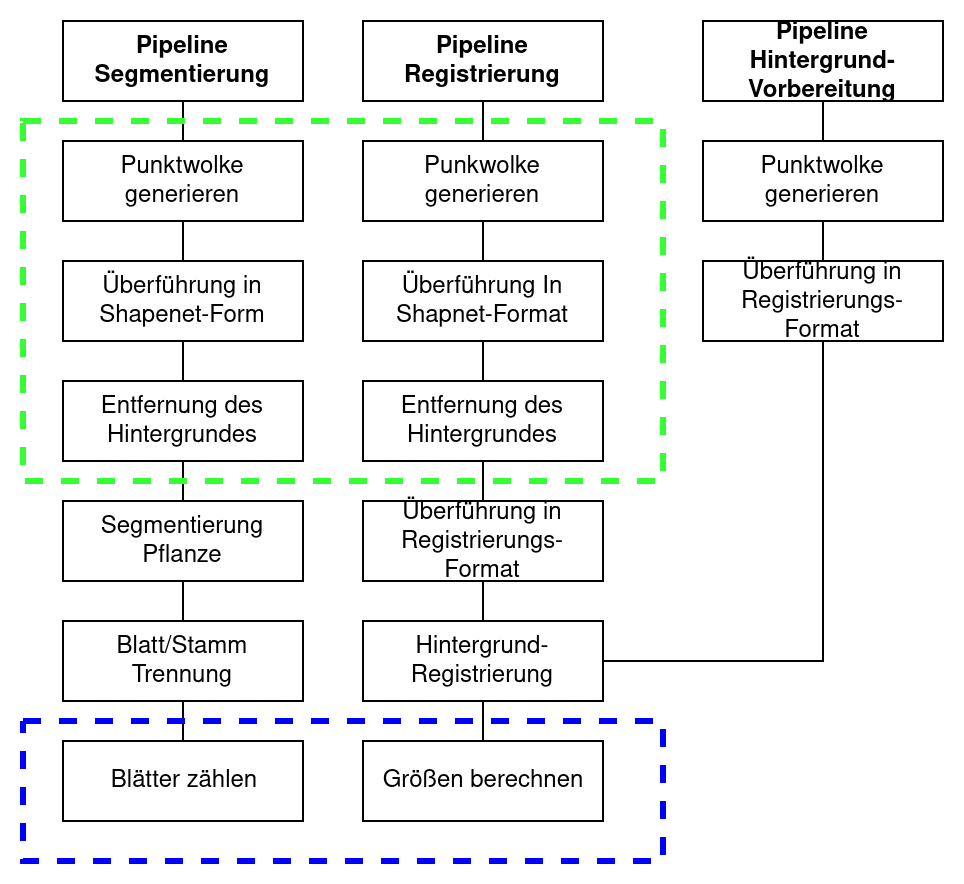
\includegraphics[width=0.65\textwidth]{./Images/Pipelines.png}
    \caption{Übersicht über die einzelnen Pipelines und die darin enthaltenen Jobs. Die Striche zwischen den Jobs zeigen die Abhängigkeiten der Jobs von oben nach unten.
    Die Ergebnisse der grün markierten Jobs können wieder verwertet werden. 
    Die blau markierten Jobs sind nicht Teil der Pipeline, aber sollen den praktischen Anwendungszweck der Pipeline-Ergebniss verdeutlichen.}
    \label{fig:Pipelines}
\end{figure}

\textbf{Punkwolke generieren}

Die Punktwolke wird auf Basis der hochgeladenen Bilder zu einem Zeitstempel generiert. 
Beim Anlegen eines neuen Zeitstempels wird die Pipeline automatisch gestartet, kann aber auch manuell neu gestartet werden, sollte es während der Generierung zu einem Server-Ausfall kommen.

\textbf{Überführung in Shapnet-Format}

%TODO: Überdenken ob Shapent-Format der richtige Name ist oder ob Segmentierungs-Format nicht zutreffender ist.

Diese Pipeline überführt die Punktwolke in das Shapenet-Format. Die Punktwolke muss in diesem Format vorliegen um beide Segmentierungs-Pipelines nutzen zu können.
Bevor die Punktwolke in das Shapenet-Format überführt wird, können zwei optionale Schritte durchgeführt werden.
Bei der Hintegrund-Segmentierung wird die Punktwolke mittels der größten in der Punktwolke zu findenden Ebene an der XY-Ebene ausgerichtet.
Bei der Pflanzen-Segmentierung werden alle als Hintergrund gelabelten Punkte entfernt. Danach beginnt die eigentliche Überführung in das Shapenet-Format.
Zuerst wird die Punktwolke so verschoben, dass die Bounding-Box im Koordinaten-Ursprung beginnt und sich auf den positiven Bereich der Achsen erstreckt.
Danach wird die Punktwolke in der Form normiert, dass sich alle Punkte der Punktwolke zwischen den Punkten $(0,0,0)$ und $(1,1,1)$ befinden.
Zuletzt werden $n=16384$ Punkte aus der Punktwolke zufällig gezogen, wobei die Punkte nicht zurück gelegt werden.

\textbf{Entfernung des Hintergrundes}

Die im Shapenet-Format vorliegende Punktwolke wird mit der Instanz von PointNet++ für die Hintegrund-Segmentierung segmentiert. Das Ergebnis wird im Speicher des Host-Systems abgelegt.
Da die Segmentierung etwas verrauscht ist wird das Ergebnis mit einem nächste Nachbarn Vote verbessert.
Im Anschluss wir das Ergebnis auf die originale Punktwolke übertragen, da sonst zu wenig Punkte für die Segmenetierung der Pflanze übrig bleiben.
Auch der Hintegrund wird entfernt und aus den verbleibenden Punkten, die nun nur noch Pflanzen-Punkte enthalten, wieder eine Punktwolke im Shapenet-Format erstellt.
Um die als Pflanze erkannten Punkte auf die originale Punktwolke zu übertragen, wird zu jedem Punkt der als Pflanze erkannt wird, in einem Radius $r$ in der originalen Punktwolke nach Punkten gesucht 
und die gefundenen Punkte in die neue Punktwolke, die nur die Punkte der Pflanze enthält, übertragen. 
Die verbleibenden Punkte in der Original-Punktwolke, die nur noch Hintergrund enthalten, werden auch gespeichert, um diese später für die Registrierung zu nutzen.

%TODO: Erleutern wie das Segmentierungs-Ergebnis auf die originale Punktwolke übertragen wird. Auch erwähnen das eine Punktwolke die nur den Hintergrund enthält für die Registrierung gespeichert wird.

\textbf{Segmentierung Pflanze}

Auf dem Ergebnis der Hintergrund-Entfernung wird PointNet++ zur Segmentierung der Pflanze gestartet. Auch hier wird das Ergebnis im Speicher des Host-Systems abgegelegt. 
Wieder wird das Segmentierungs-Ergebnis wie bei der Hintergrundentfernung verbessert. Im Falle der Pflanzen-Segmentierung ist dieser Schritt nicht zwangläufig nötig, da die Ergebnisse gut genug sind.

\textbf{Blatt/Stamm Trennung}

Die Punktwolke die die segmentierte Pflanze enthält wird in zwei Punktwolken aufgeteilt, 
wobei die eine Punktwolke nur noch Punkte enthält, die Blätter repräsentieren und eine, die nur noch Punkte enthält, die Stiele repräsentieren.

\textbf{Blätter zählen}

Die Punktwolke $P$ die die Blätter enthält wird nun mit einer 3D Interpretation des Flood-Fill-Algoritmus untersucht. Hierbei wird ein zufälliger Punkt in der Punkwolke gewählt und in die Menge $Q$ aufgenommen.
Nun wird solange bis $Q$ keine Punkte mehr enhält ein Punkt $p$ aus $Q$ entnommen und mittels nächster Nachbarn-Suche im Radius $r$ nach weiteren Punkten in der Nähe gesucht. Gefundene Punkte werden in $Q$ aufgenommen, wenn sie nicht in $B$ enthalten sind.
Der Punkt $p$ wird danach in die Menge $B$ aufgenommen. Ist $Q$ leer, wird die Menge $B$ aus $P$ entfernt und der Blatt-Zählstand um eins erhöht. 
Der Vorgang wird so lange wiederholt, bis keine Punkte mehr in $P$ enthalten sind.

\textbf{Überführung in Registrierungs-Format }

Zuerst wird die Punktwolke wieder anhand der größten Ebene, die in der Punktwolke zu finden ist, an der XY-Ebene ausgerichtet.
Dabei kann es sich entweder um die Punktwolke des Hintergrundes oder der bei der Entfernung des Hintergrundes übrig gebliebene Punktwolke eines Zeitstempels handeln.
Danach wird um das Zentrum der Punktwolke ein Ausschnitt entnommen. 
Im folgenden wird die Punktwolke wie beim Shapenet Format normiert und es werden zufällig $n=1024$ Punkte aus der Punktwolke gezogen.

\textbf{Hintergrund-Registrierung}

Um einen Zeitstempel $t$ einer Messung mit dem Hintergrund der Messreihe zu registrieren, muss sowohl die Punktwolke $P_t$ für den Zeitstempel $t$ als auch die Punktwolke für den Hintegrund im Registrierungs-Format vorliegen.
Ist das gegeben, kann die Registrierung gestartet werden. Hierbei wird ein Skalierungs-Faktor $s$ und eine Transformation $T$ ermittelt. 
Das Registrierungs-Ergebnis $P_{Registration}$ der Punktwolke $P_t$ kann dann mit der Formel $P_{Registration} = (P_t \cdot s) \cdot T$ ermittelt werden. 
Wobei beachtet werden muss, dass zuerst die Skalierung und dann die Transformation angewandt wird.

\textbf{Größen berechnen}

Ist die Punktwolke $P_t$ zum Zeitstempel $t$ mit dem Hintegrund registriert, können die Größen Höhe und Volumen nun leicht berechnet werden.
Die Höhe kann über den höchsten z-Wert der Punkte in $P_t$ ermittelt werden. Um das Volumen zu berechnen, muss für $P_t$ die Länge $l$, Breite $b$ und Höhe $h$ ermittelt werden (siehe Gleichungen \ref{eq:length} - \ref{eq:height}). 
Das Volumen $v$ lässt sich dann folgendermaßen berechnen: $v = h \cdot b \cdot l$.

\begin{equation}
    \label{eq:length}
    l = \left\{
    \begin{array}{ll}
    |minX| + maxX & minX \leq 0 \\
    maxX - minX & \, \textrm{sonst} \\
    \end{array}
    \right. 
\end{equation}

\begin{equation}
    \label{eq:width}
    b = \left\{
    \begin{array}{ll}
    |minY| + maxY & minY \leq 0 \\
    maxY - minY & \, \textrm{sonst} \\
    \end{array}
    \right. 
\end{equation}

\begin{equation}
    \label{eq:height}
    h = \left\{
    \begin{array}{ll}
    |minZ| + maxZ & minZ \leq 0 \\
    maxZ - minZ & \, \textrm{sonst} \\
    \end{array}
    \right. 
\end{equation}

Ist die Höhe für den vorherigen Zeitstempel $t-1$ auch bekannt, kann das relative Wachstum seit dem letzten Zeitpunkt ermittelt werden. Dieser Schritt kann nicht für den ersten Zeitstempel ausgeführt werden.

\begin{figure}
    \centering
    \begin{minipage}{0.3\textwidth}
        \centering
        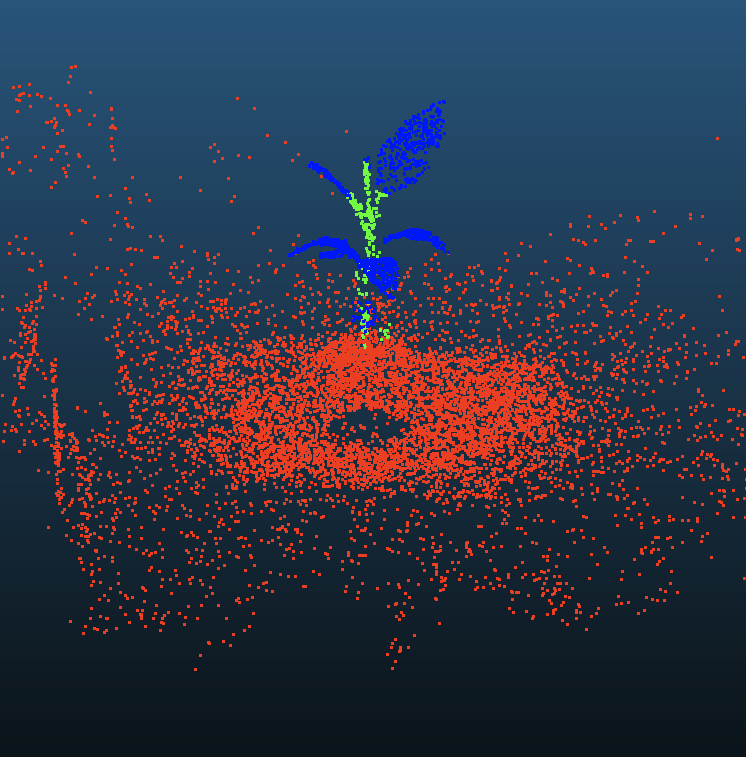
\includegraphics[height=4.5cm,width=4.5cm]{./Images/PipelineBackgroundSegmentationStriped.png}
        \caption{Hintegrund-Segmentierung}
        \label{fig:PiplineBackgroundSegmentation}
    \end{minipage}\hfill
    \begin{minipage}{0.3\textwidth}
        \centering
        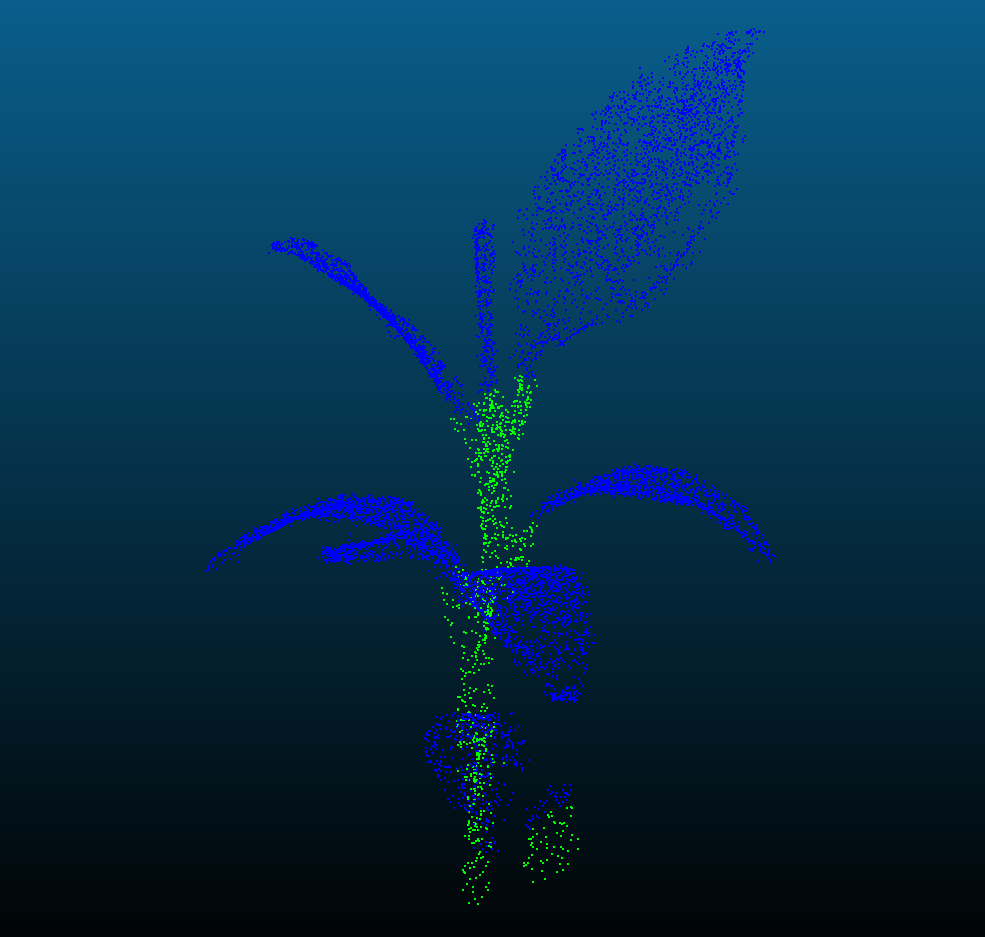
\includegraphics[height=4.5cm,width=4.5cm]{./Images/PipelinePlantSegmentation.png}
        \caption{Planzen-Segmentierung}
        \label{fig:PipelinePlantSegmentation}
    \end{minipage}\hfill
    \begin{minipage}{0.3\textwidth}
        \centering
        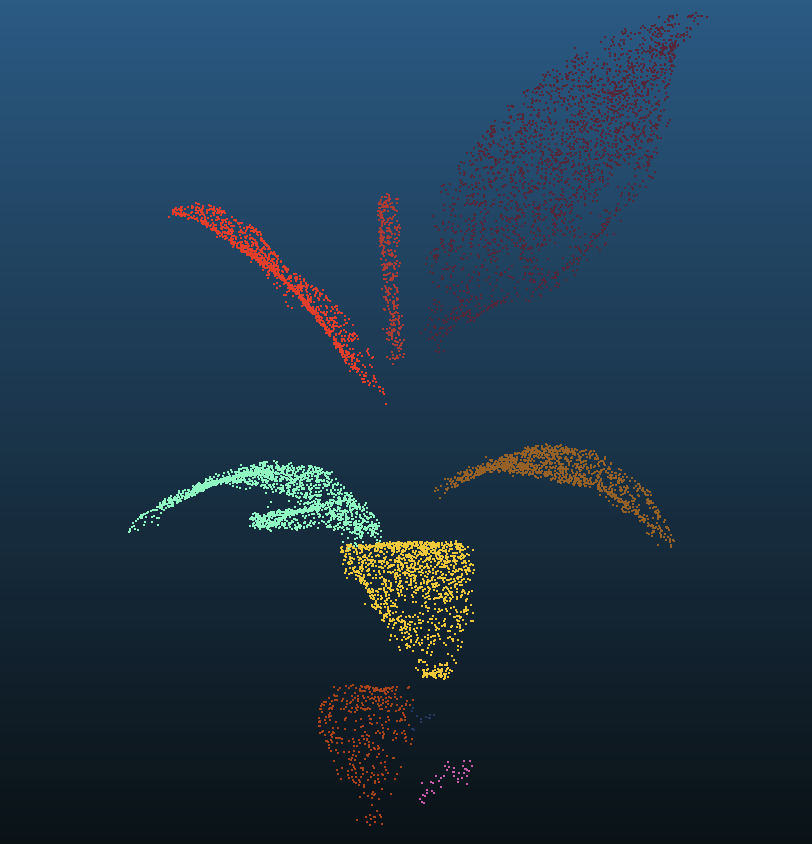
\includegraphics[height=4.5cm,width=4.5cm]{./Images/PipelineLeaveSegmentationStriped.png}
        \caption{Blatt-Segmentierung}
        \label{fig:PipelineLeaveSegmentation}
    \end{minipage}
\end{figure}

\newpage
\section{Ergebnisse}
%-------------------------------------------------------------
\label{sec:ergebnisse}
%Hierhin gehört eine Beschreibung der von Ihnen durchgeführten Tests zur
%Verifikation bzw.~Qualitätssicherung Ihrer Lösung. Wenn Sie Messungen
%durchgeführt haben, so stellen Sie die Ergebnisse hier in Tabellen und
%Diagrammen dar.
%
%Auch die Diskussion der Messergebnisse oder der Besonderheiten der
%Testergebnisse gehört hierher.

\subsection{Vergleich von Verfahren zur Generierung von 3D-Punktwolken auf Basis von Bildern}

Um eine geeignete Anwendung zur Generierung von 3D-Punktwolken auszuwählen, muss erst entschieden werden, nach welchen Gütekriterien verschiedene Verfahren betrachtet werden sollen und wie wichtig diese sind.
Bei dieser Arbeit ist die nötige Anzahl der Bilder, die zur Generierung einer Punktwolke mit genug Information nötig sind, sowie die Dauer die Punktwolke zu generieren die wichtigsten Kriterien.

Um zu messen wie viele Bilder benötigt werden, um eine Szene gut zu repräsentieren muss ein Goldstandart von der fotografierten Szene als 3D-Punktwolke erstellt werden, mit dem verglichen werden kann.
Dieser Goldstandart kann erstellt werden, indem alle Fotografien, einer Pflanze zu einem Zeitpunkt, die zur Verfügung stehen genutzt werden und damit alle Verfahren eine Punktwolke erstellen lassen. 
Unter den erstellten Punktwolken kann die ausgesucht werden, die die Szene am besten repräsentiert. 
Das trifft auf die Punkwolke zu die den höchsten Detail-Grad hat und möglichst wenig Fehler, wie fehlende Teile der Szene oder Rauschen enthält.
Die gewählte Punktwolke sollte nachbearbeitet werden, um etwaige Fehler wie Rauschen manuell zu entfernen.

Nun kann mit wenigeren Bildern aus demselben Datensatz ein weitere Punktwolke generiert werden und die Distanz der Punkte der Goldstandart-Punktwolke zum jeweils nächsten Punkt der erstellten Punktwolke gemessen werden.
Die Summe dieser Abstände kann als Fehlermaß genutzt werden. Bei der Berechnung der Abstände muss beachtet werden, dass die Punkwolken mit dem Goldstandart registriert sind.

Nach einem manuellen Auswahlverfahren sind ODM und Colmap als geeignete Anwendung zur Generierung von Punktwolken gewählt worden, 
da diese die einzigen untersuchten Anwendungen sind, die bei wenig Bildern gute Ergebnisse erzielen, die die Szene mit allen wichtigen Details erkennen lassen.
Für die manuelle Auswertung wurden auf einer Menge von 25 Bildern die Implementationen ODM, Colmap, OpenCV SfM-Pipeline, Meshroom (nutzt AliceVision) und OpenMVG miteinander verglichen. 
Die generierten Punktwolken sind in Abbildung \ref{fig:SfM:All:Compare} zu sehen.
Es ist deutlich zu erkennen, dass bis auf Colmap und ODM alle anderen Verfahren schwerwiegende Probleme in der Representation haben. Meshroom hat Probleme, feine Strukturen zu erkennen. 
OpenMVG generiert zu wenig Punkte und OpenCV hat ein Problem bei der Berechnung der Kamera-Kalibrierung wodurch es zu Fehlern bei der Rekonstruktion kommt.
\begin{figure}
    \centering
    \begin{subfigure}[t]{1.0\textwidth}
        \centering
        \raisebox{-\height}{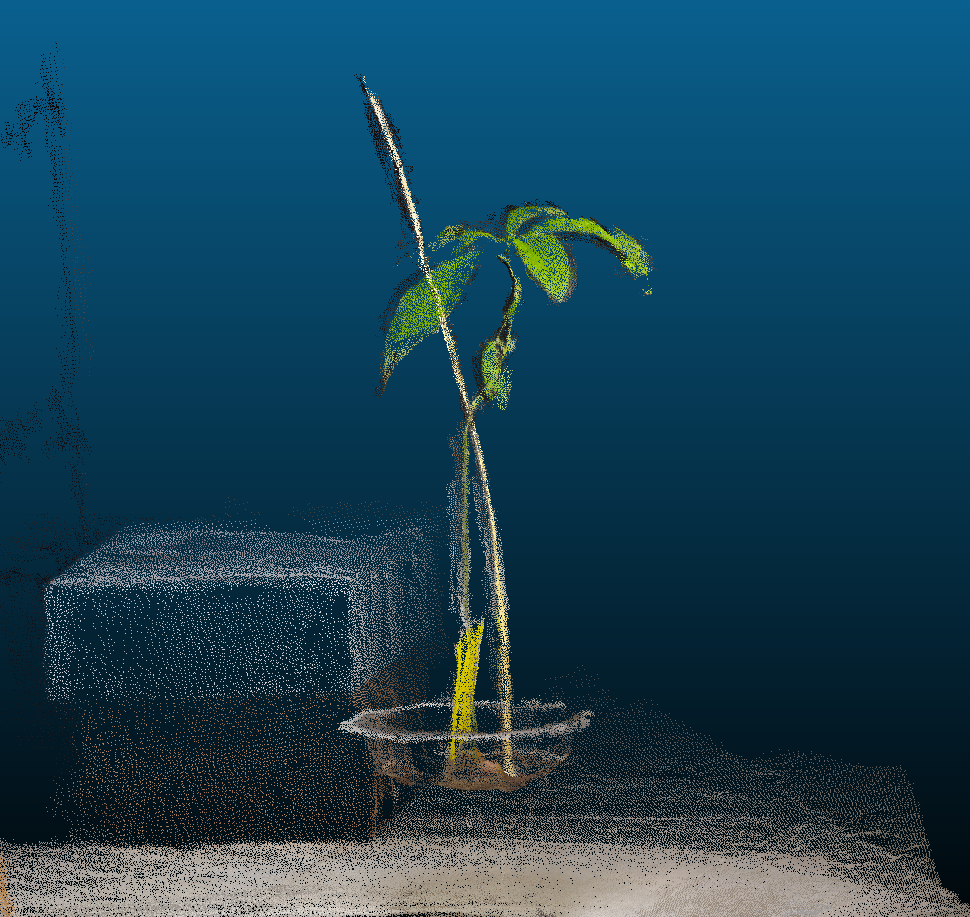
\includegraphics[width=\imageSizeThree, height=\imageSizeThreeHeight]{./Images/PointCloudGeneration_odm.png}}
        \centering
        \raisebox{-\height}{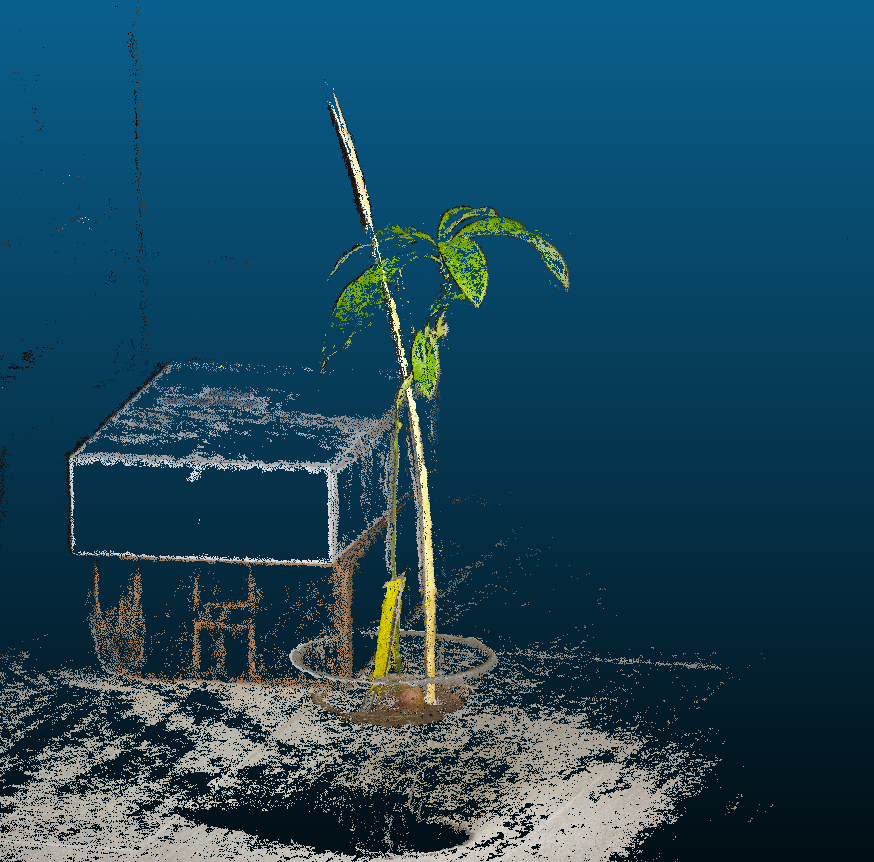
\includegraphics[width=\imageSizeThree, height=\imageSizeThreeHeight]{./Images/PointCloudGeneration_colmap.png}}
        \vspace{.6ex}
        \centering
        \raisebox{-\height}{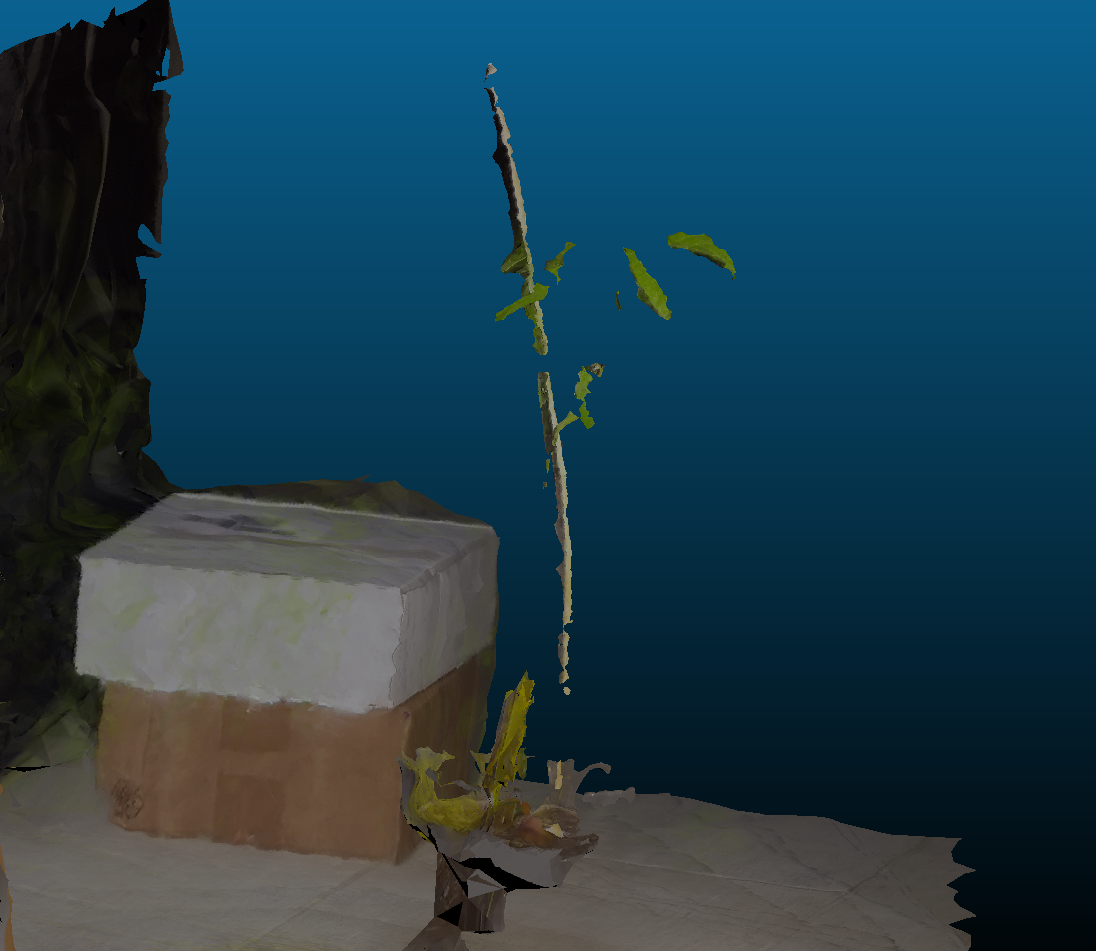
\includegraphics[width=\imageSizeThree, height=\imageSizeThreeHeight]{./Images/PointCloudGeneration_meshroom.png}}
        \centering
        \raisebox{-\height}{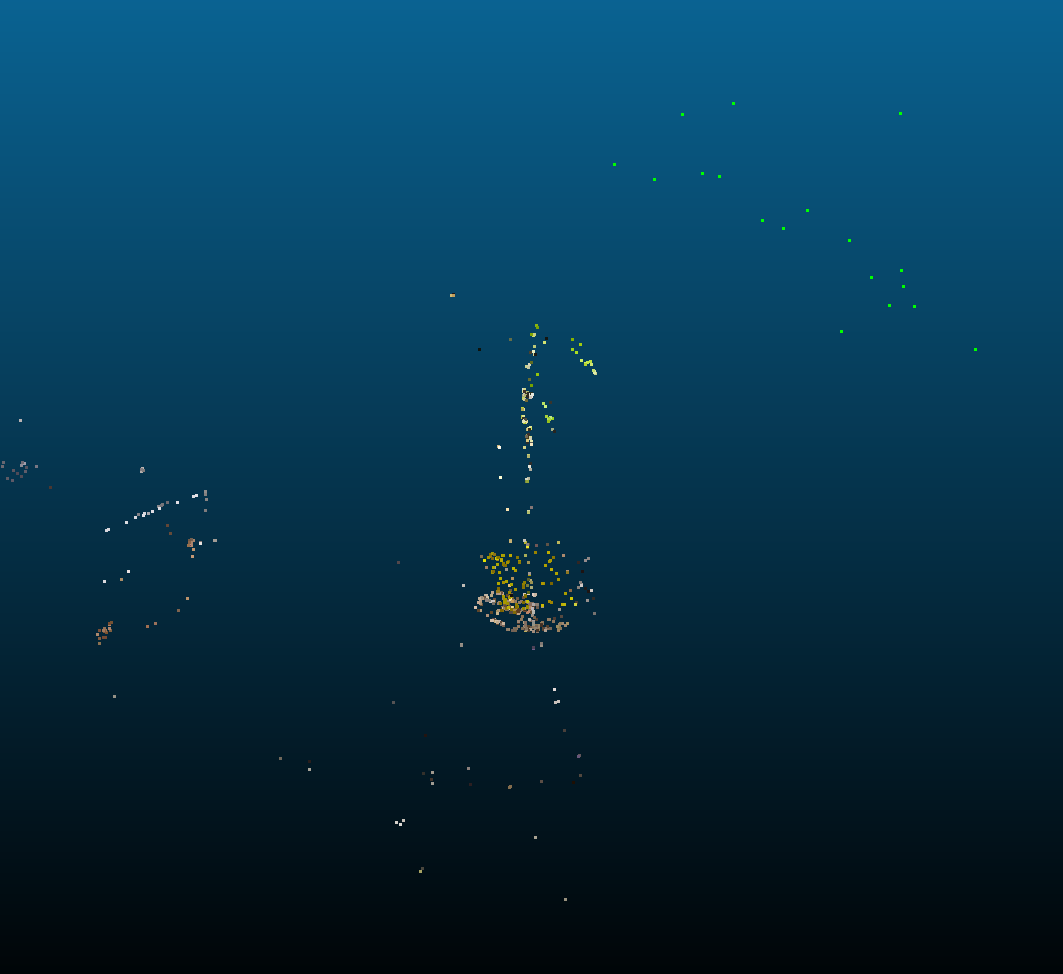
\includegraphics[width=\imageSizeThree, height=\imageSizeThreeHeight]{./Images/PointCloudGeneration_openmvg.png}}
        \centering
        \raisebox{-\height}{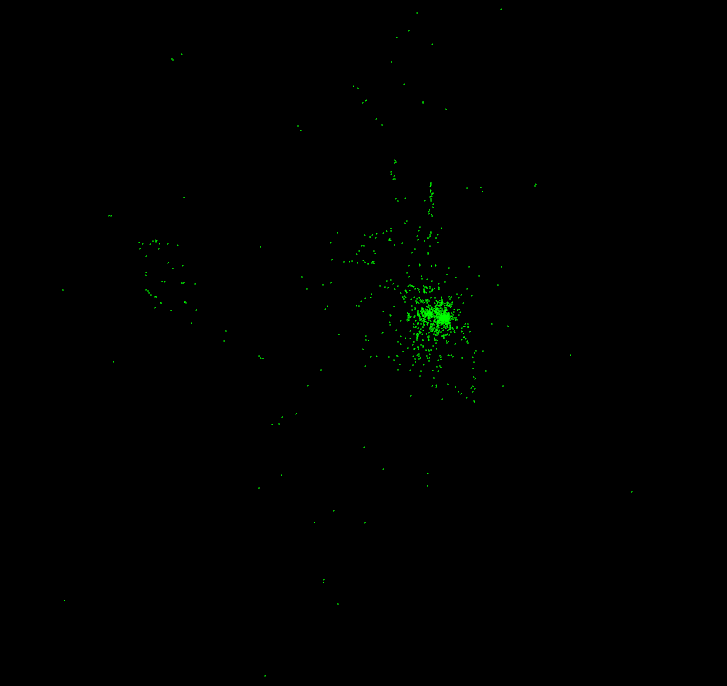
\includegraphics[width=\imageSizeThree, height=\imageSizeThreeHeight]{./Images/PointCloudGeneration_opencv.png}}
    \end{subfigure}
    \caption{Ergebnisse auf Datensatz mit 25 Bildern. Von oben links nach unten rechts: ODM, Colmap, Meshroom, OpenMVG, OpenCV}
    \label{fig:SfM:All:Compare}
\end{figure}

Zum weiteren Vergleich beider Anwendungen werde aus 73 Bildern sowohl mit Colmap als auch mit ODM eine Punktwolke generiert, 
da ODM die Szene besser repräsentiert und weniger Rauschen beinhaltet, wurde die mit ODM erstellte Punktwolke als Goldstandart gewählt. 

Im Folgenden werden aus Teilmengen der Bilder jeweils für ODM und Colmap Punktwolken generiert. Die Teilmengen bestehen aus 5 bis 70 Bildern, wobei immer 5 Bilder mehr pro Schritt genutzt werden.
Bei der Wahl der Bilder pro Schritt wird beachtet, dass die Bilder ähnliche Ausschnitte enthalten, da diese zur Generierung von Punktwolken nötig sind.

In zwei Vergleichen wurden zum einen die durschnittliche Distanz für jeden Punkt zum nächsten Punkt in der Goldstandart-Punktwolke verglichen und zum anderen die Anzahl generierter Punkte pro Schritt.
Die Ergebnisse sind in Abbildung \ref{fig:DistanceCloudGen} und \ref{fig:NPointsCloudGen} zu sehen. 
Es ist zu erkennen, dass Colmap zwar mehr Punkte generiert als ODM, aber ab einer bestimmten Anzahl Bilder überwiegt das Rauschen in den mit Colmap generierten Puntkwolken so stark, dass der Abstand zur Goldstandart-Punktwolke größer als der mit ODM erreichte Abstand wird.

\begin{figure}
    \centering
    \begin{minipage}{0.475\textwidth}
        \centering
        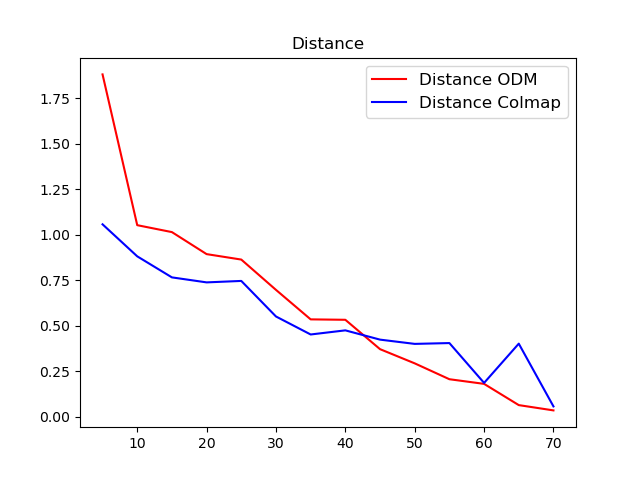
\includegraphics[width=1.0\textwidth]{./Images/DistanceCloudGen.png}
        \caption{Distanz der Punktwolke mit bestimmter Anzahl Bilder zur Goldstandart-Punktwolke.}
        \label{fig:DistanceCloudGen}
    \end{minipage}\hfill
    \begin{minipage}{0.475\textwidth}
        \centering
        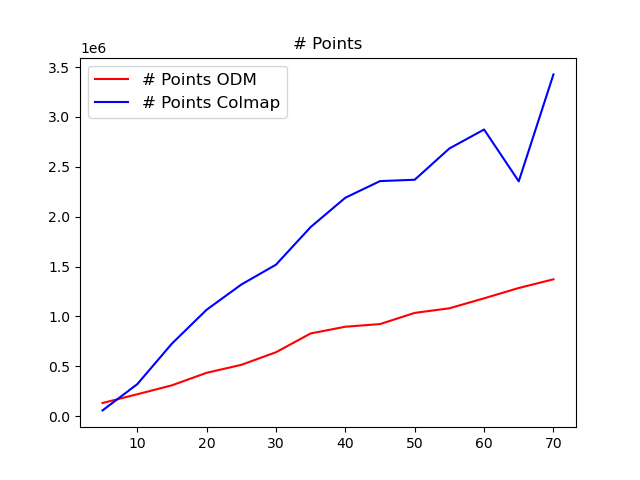
\includegraphics[width=1.0\textwidth]{./Images/NPointsCloudGen.png}
        \caption{Anzahl Punkte die mit einer bestimmten Anzahl Bilder generiert werden kann.}
        \label{fig:NPointsCloudGen}
    \end{minipage}
\end{figure}

Generell lässt sich in den generierten Punktwolken beobachten, dass Colmap mehr Rauschen enthält als ODM. Exemplarisch zeigen dies Abbildungen \ref{fig:ODMNoise} und \ref{fig:ColmapNoise}. 
Ein Nachteil von ODM ist, dass um die Kannten herum sehr viele Hintergrundpunkte mit aufgenommen werden, die eine Art Halo um die erkannten Strukturen bilden. 
Dadurch können feine Strukturen ineinander über fließen. Dies ist auch bei Colmap zu beobachten, allerdings nur in einem kleineren Ausmaß.
Bei Colmap hat man zusätzlich das Problem, dass es zu größeren Lücken in erkannten Oberflächen kommt.
Beide Probleme sind in Abbildung \ref{fig:ODMerror} und \ref{fig:ColmapError} zu sehen. 
Des weiteren kann es vorkommen, dass Colmap zwei Szenen in den Bildern erkennt, was insbesondere bei Nutzung von vielen Bildern vorkommt (Abbildung \ref{fig:ColmapDuplicatedScene}).

\begin{figure}
    \centering
    \begin{minipage}{0.475\textwidth}
        \centering
        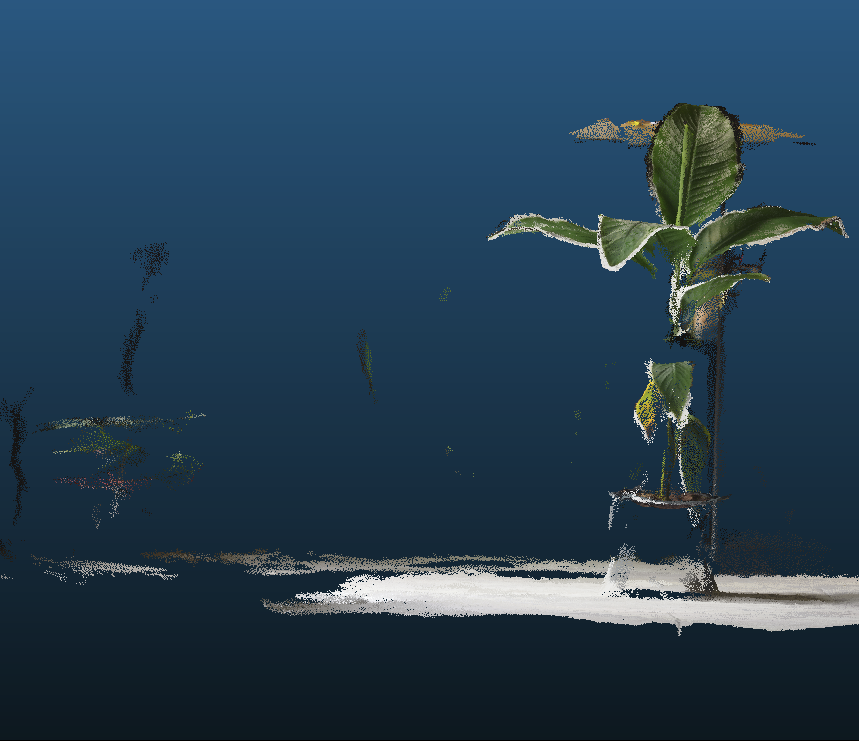
\includegraphics[width=1.0\textwidth]{./Images/ODMNoise2.png}
        \caption{ODM mit 40 Bildern - Ansicht von der Seite}
        \label{fig:ODMNoise}
    \end{minipage}\hfill
    \begin{minipage}{0.475\textwidth}
        \centering
        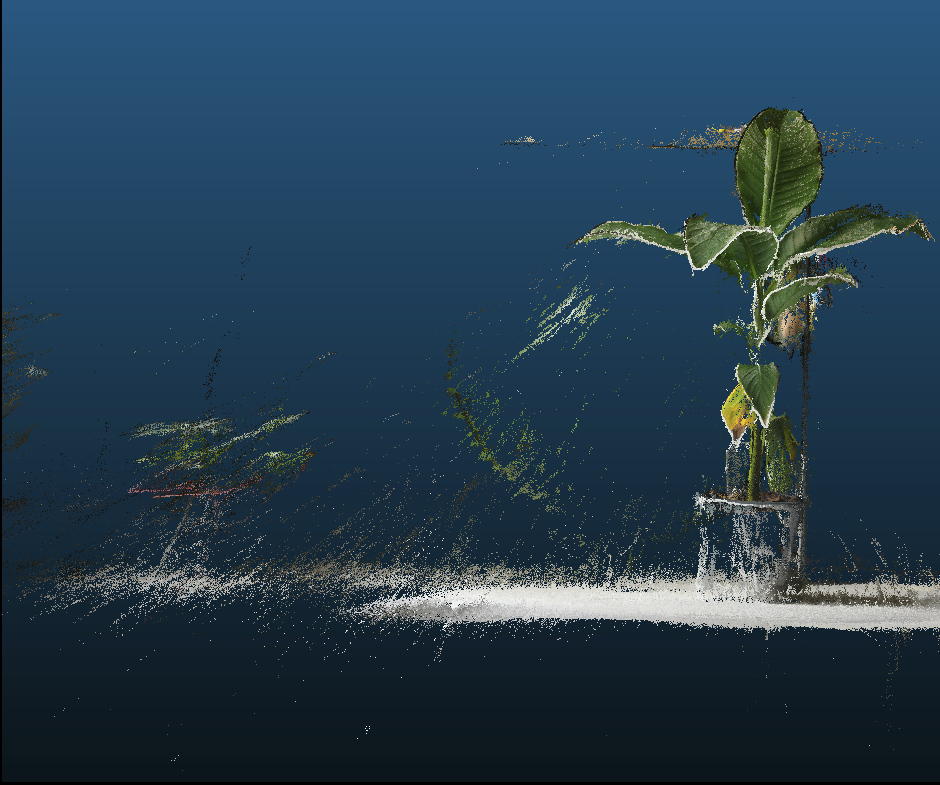
\includegraphics[width=1.0\textwidth]{./Images/ColmapNoise2.png}
        \caption{Colmap mit 40 Bildern - Ansicht von der Seite}
        \label{fig:ColmapNoise}
    \end{minipage}
\end{figure}

\begin{figure}
    \centering
    \begin{minipage}{0.475\textwidth}
        \centering
        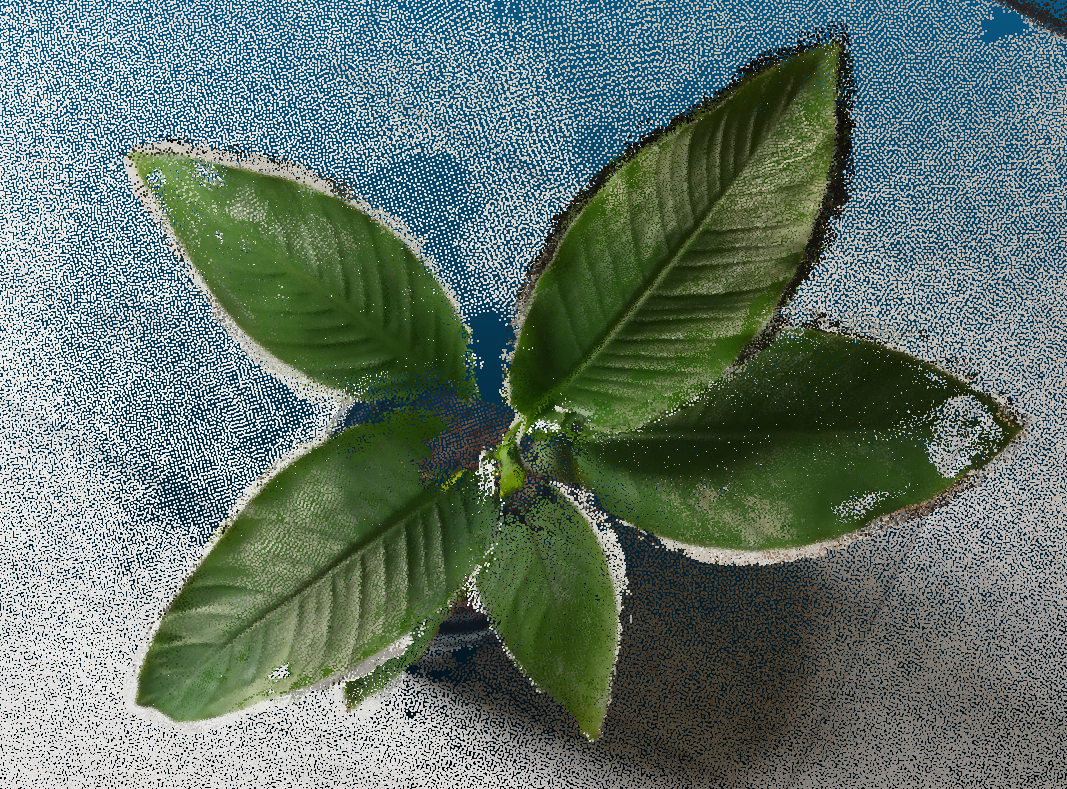
\includegraphics[width=1.0\textwidth]{./Images/ODMError.png}
        \caption{ODM mit 40 Bildern - Ansicht von Oben}
        \label{fig:ODMerror}
    \end{minipage}\hfill
    \begin{minipage}{0.475\textwidth}
        \centering
        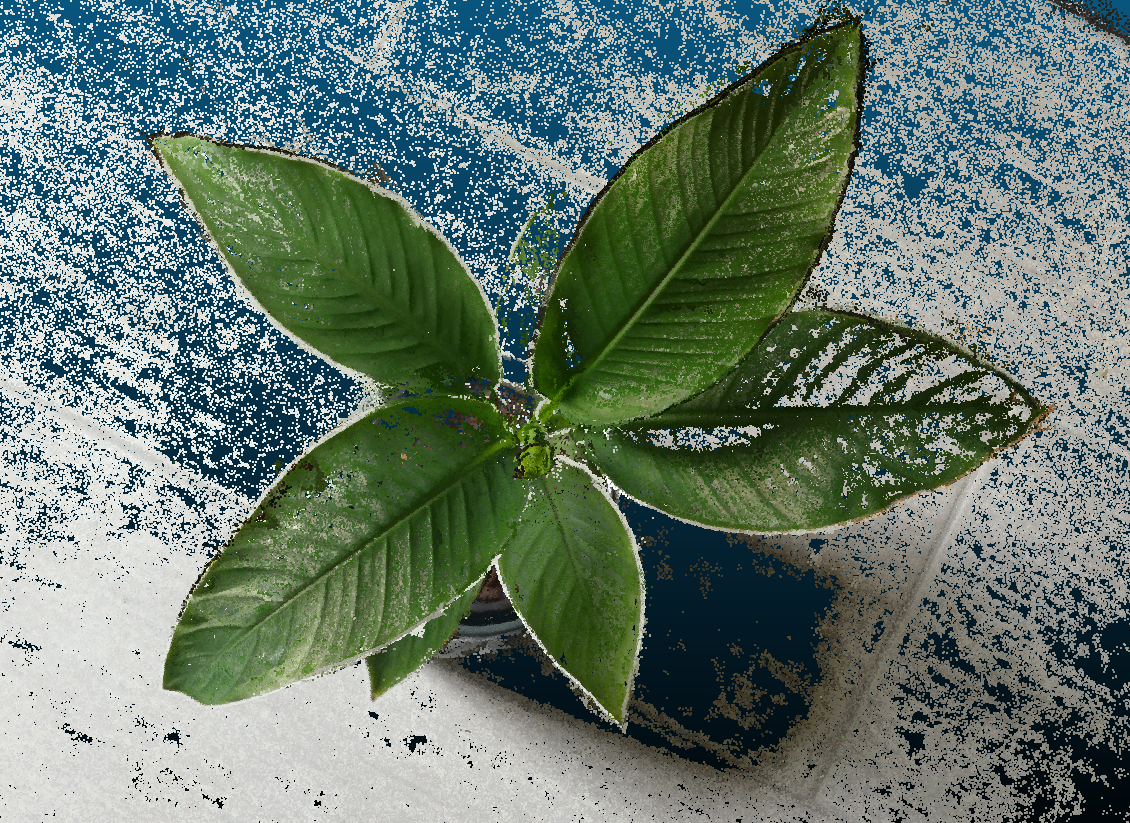
\includegraphics[width=1.0\textwidth]{./Images/ColmapError.png}
        \caption{Colmap mit 40 Bildern - Ansicht von Oben}
        \label{fig:ColmapError}
    \end{minipage}
\end{figure}

\begin{figure}
    \centering
        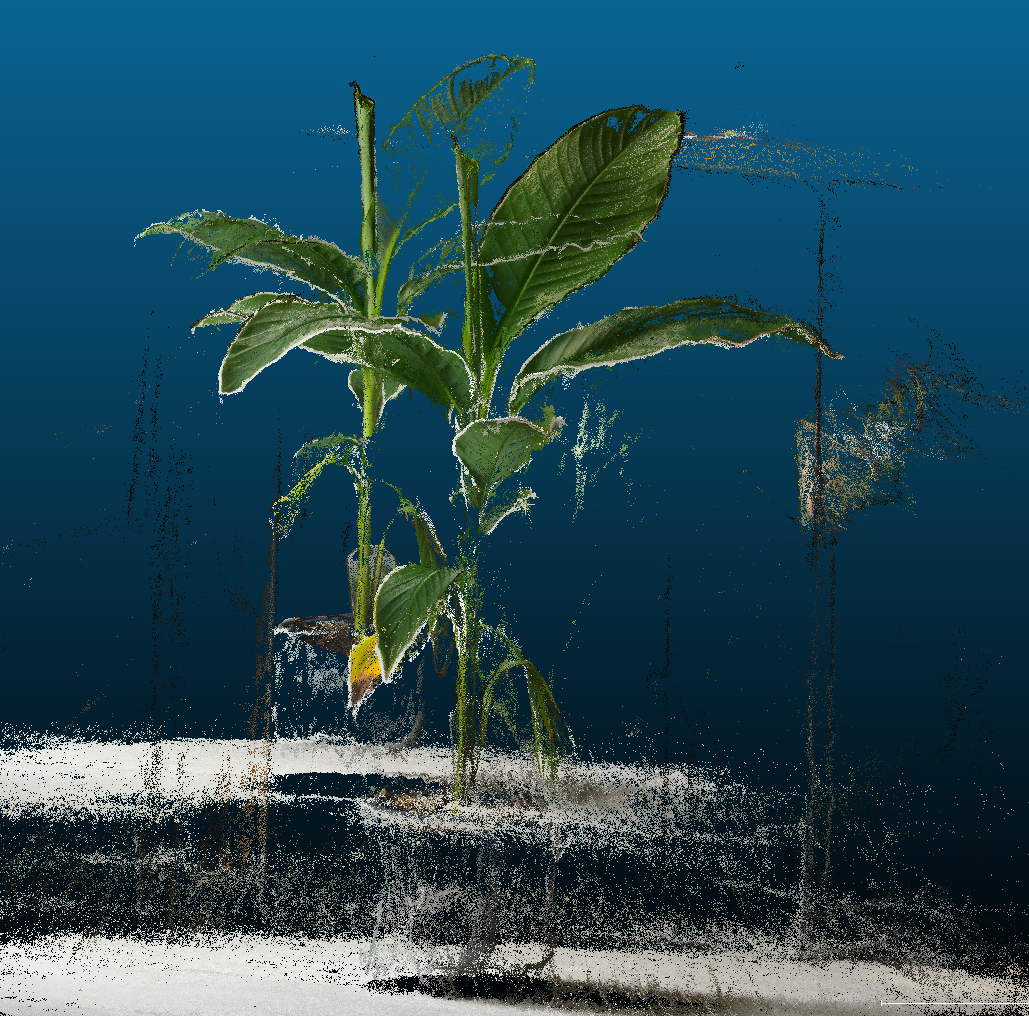
\includegraphics[width=0.5\textwidth]{./Images/ColmapDuplicatedScene.png}
        \caption{Colmap mit 55 Bildern und doppelt erkannter Szene.}
        \label{fig:ColmapDuplicatedScene}
\end{figure}

Ein weiterer Punkt bei der Bewertung des Verfahrens zur Generierung von 3D Punktwolken ist die Zeit, die benötigt wird, die Punkwolke zu generieren.
Hier dominiert ODM klar. 
Obwohl, mangels der GEO-Position der Bilder, ODM nur in der Lage ist die CPU parallel zu nutzen und nicht die GPU, werden die Punkwolken wesentlich schneller generiert als mit Colmap, welches die GPU nutzt und diese auch gut auslastet.
ODM benötigt zur Generierung einer Punktwolke mit $73$ Bilder $566$ Sekunden, wärend Colmap für die gleiche Datenbasis $4148$ Sekungen benötigt. 
Sollten GEO-Positionen für die Bilder bekannt sein, kann ODM die GPU nutzen und somit die Zeit die benötigt wird, die Punktwolken zu generieren, weiter verbessern.

Da ODM wesentlich weniger Rauschen beinhaltet, keine Probleme mit doppelt erkannten Szenen hat und weniger Zeit zur Generierung der Punkwolken benötigt wird in dieser Arbeit ODM zur Generierung von Punktwolken ausgewählt, 
wobei die Dauer, die zur Generierung der Punktwolke benötigt wird, der ausschlaggebende Faktor für die Entscheidung ist.

\subsection{Vergleich von Verfahren zur Registrierung 3D-Punkwolken}

Die Annahmem, dass DCP eine gute Schätzung für die Transformations-Matrix liefern kann hat sich, auch nach umfangreichem Training, nicht bestätigt, 
auch konnte durch den ersten Ansatz über ICP keine gute initiale Schätzung gefunden werden sodass die Skalierung erfolgreich ermittelt werden konnte.
Lediglich der letzte Ansatz hat sich in Experimenten als relativ robust heraus gestellt. Daher sollen die verschiedenen Verfahren miteinander verglichen werden.

In einem ersten Schritt wurden verschiedene Lösungen aus dem Deep-Learning Bereich miteinander verglichen. 
Es wird die Distanz zwischen transformierter Quell-Punktwolke und Ziel-Punktwolke, wie im Abschnitt \ref{sec:realisierung:implementierung2} beschrieben, gemessen. 
Neben der Distanz berichten wir über den bei der Evaluation gemessenen Loss.
Die einzelnen Verfahren sind alle in dem Python-Paket learning3d \cite{learning3d} implementiert, nutzen die selbe Datenbasis ModelNet40 für das Training und sind somit gut vergleichbar. 
Für DCP und RPM-Net wurde das vortrainierte Model vom Author des Pakets genutzt.
PointNetLK musste trainiert werden und wurde mit den empfohlenen Angaben des Authors trainiert. 
Die Evaluation wurde drei mal mit zufälligen Daten wiederholt und aus den drei Durchläufen die Mittelwerte für die ermittelten Werte gebildet.
Die Ergebnisse sind in Tabelle \ref{tab:registration:deeplearn:compare} veranschaulicht.

\begin{table}
\begin{center}
\begin{tabular}{|l || c | c | c | } 
    \hline
     & DCP & RPM-Net & PointNetLK \\  
    \hline
    \hline
    Distanz & $0,0292$ & $0,0663$& $0,026$\\
    \hline
    Loss & $0,922$& $0,061$& $0,111$\\
    \hline
\end{tabular}
\end{center}
\caption{Vergleich von Registrierungs-Verfahren auf ModelNet40. Distanz und Loss sind jeweils Mittelwerte über alle Datensätze in der Iteration.}
\label{tab:registration:deeplearn:compare}
\end{table}

In einem zweiten Schritt werden die Verfahren, auf Basis konkreten Beispielen der Problemstellung, miteinander verglichen. 
Neben DCP, RPM-Net und PointNetLK wird auch die ICP Implementation aus dem Python-Paket open3d \cite{zhou2018open3d} und eine weitere in c++ implementierte ICP Version RICP verglichen.
Hier werden exemplarisch je eine Avocado- und eine Bananen-Pflanze verglichen. Wie im vorherigen Vergleich wird die Distanz zur Zielpunktwolke in den Ergebnissen wieder gegeben.
Die Ergebnisse sind in Tabelle \ref{tab:registration:real:compare} zu sehen

\begin{table}
    \begin{center}
    \begin{tabular}{|l || c | c | c | c | c | } 
        \hline
         & DCP & RPM-Net & PointNetLK & ICP & RICP \\  
        \hline
        \hline
        Banane & $0.0585$ & $0.0129$& $0.1673$& $0.0117$& $0.0178$\\
        \hline
        Avocado & $0.0721$& $0.012$& $0.2235$& $0.0122$& $0.0245$\\
        \hline
    \end{tabular}
    \end{center}
    \caption{Vergleich von Registrierungs-Verfahren auf konkreten Beispielen der Problemstellung. Für jede Pflanze wird die Distanz zwischen Quelle und Ziel angegeben}
    \label{tab:registration:real:compare}
\end{table}

lassen erkennen, dass ICP die besten Ergebnisse für die Registrierung liefert. 
Die Neuronalen-Netze liefern keine guten Ergebnisse. Mit Aussnahme von RPM-Net. 
Die Ergebnisse für RPM-Net liegen in etwa gleich auf mit den Ergebnissen die für ICP erreicht wurden und sind besser als die Ergebnisse von RICP.

\subsection{Vergleich von Verfahren zur Segmentierung von Pflanzen auf 3D-Punkwolken}

In Experimenten mit dem handgeschriebenen Classifier konnte keine gute Parametriesierung, die eine gute Unterteilung in Blätter und Stämme erreichen konnte, gefunden werden. 
Dies liegt in erster Linie an der Qualität der Punktwolken.
Diese haben das Problem, dass die oft sehr feinen Stiele der Pflanze nicht als Zylinder sondern als Ebene in den Punktwolken repräsentiert werden, wie in Abbildung \ref{fig:handcrafted:classifier} (oben) zu sehen ist.
Ein weiteres Problem ist eine allgemeingültige Parametriesierung zu finden, wie Abbildung \ref{fig:handcrafted:classifier} (unten) zeigt. Hier wurde mit dem selben Schwellwert klassifiziert.

\begin{figure}
    \centering
    \begin{subfigure}[t]{1.0\textwidth}
        \centering
        \raisebox{-\height}{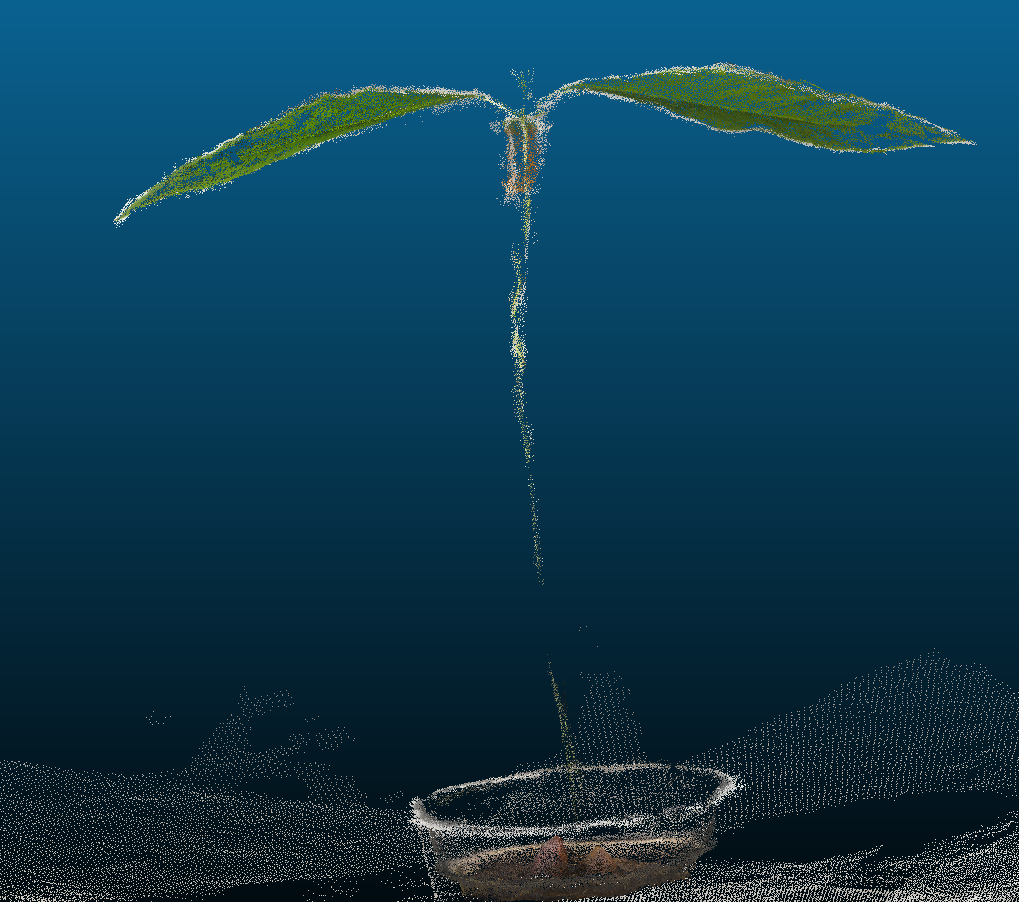
\includegraphics[width=\imageSizeTwo, height=\imageSizeTwoHeight]{./Images/OdmFlatError1.png}}
        \centering
        \raisebox{-\height}{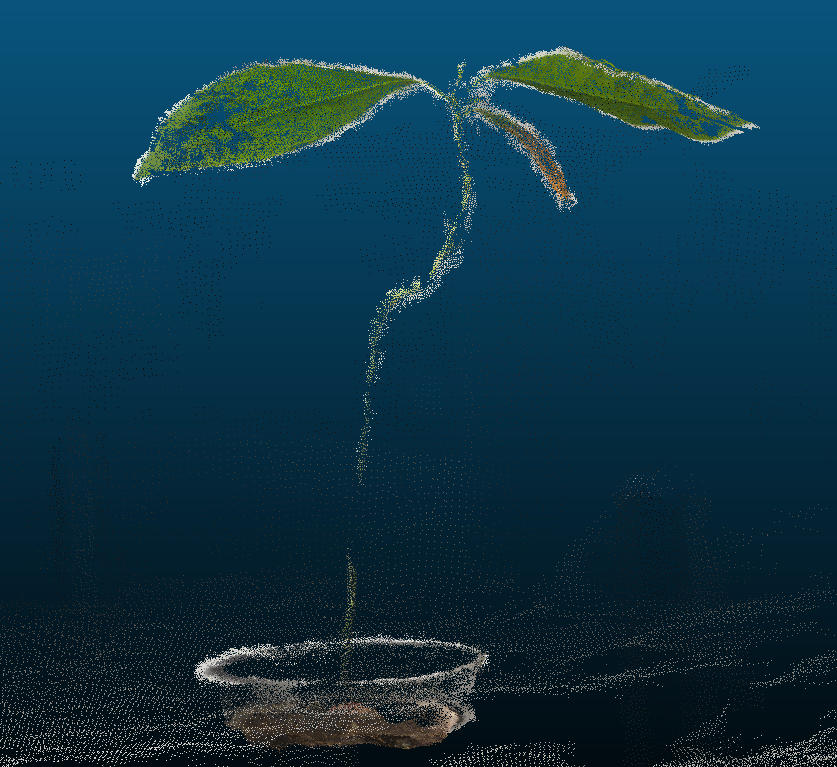
\includegraphics[width=\imageSizeTwo, height=\imageSizeTwoHeight]{./Images/OdmFlatError2.png}}
        \vspace{.6ex}
        \centering
        \raisebox{-\height}{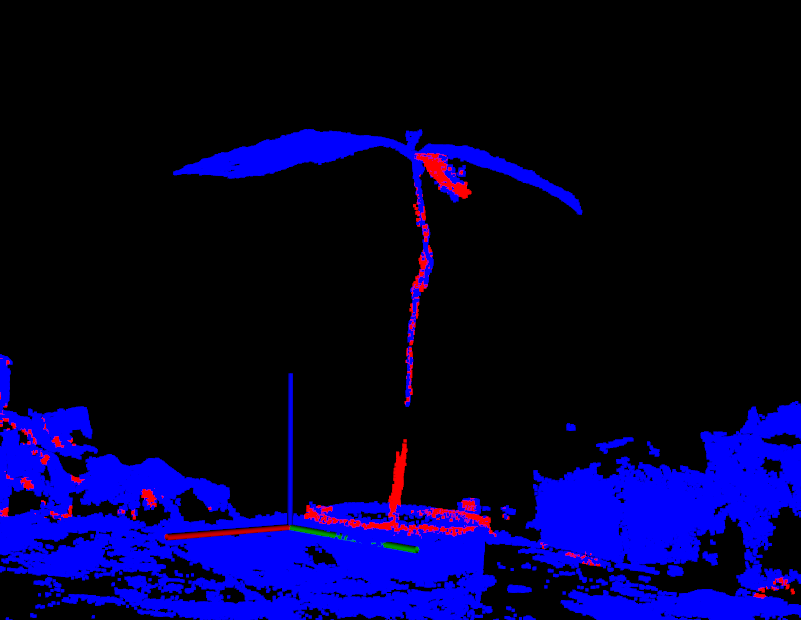
\includegraphics[width=\imageSizeTwo, height=\imageSizeTwoHeight]{./Images/HandcraftedClassifierAvocado.png}}
        \centering
        \raisebox{-\height}{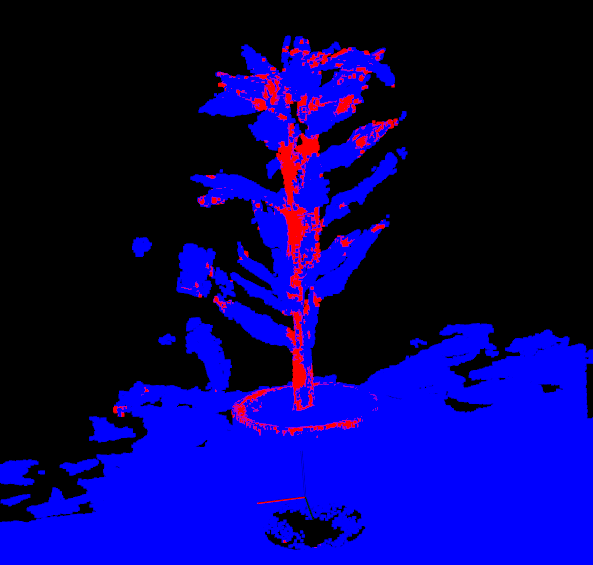
\includegraphics[width=\imageSizeTwo, height=\imageSizeTwoHeight]{./Images/HandcraftedClassifierPlant2.png}}
    \end{subfigure}
    \caption{Oben: ODM Seitenansicht die als Ebene erkannten Stiel zeigt.\\Unten: Segmentierungs-Ergebniss für zwei verschiedene Pflanzen mit dem selben Schwellwert.}
    \label{fig:handcrafted:classifier}
\end{figure}

\textbf{Datenbasis für das Training von PointNet++}

Als Datenbasis für das Training von PointNet++ wurden 144 handgelabelte Punkwolken von verschiedenen Pflanzen gewählt. Darunter sind Tomaten, Mais, Paprika, Avocado, Bananen und weitere nicht bekannte Sorten. 
Da diese Datenbasis für das Training eines Neuronalen Netzes recht klein ist, wurden aus jeder einzelnen Punktwolke bis zu 20 Subsample erstellt. 
Diese wurden so erstellt, dass zufällig $n$ Punkte aus einer Punktwolke gezogen und entfernt wurden.
Des weiteren sind die Daten so aufbereitet, dass der Boden der Punktwolke an der XY-Ebene ausgerichtet ist und der Stiel bei geradem Wachstum Richtung z-Achse zeigt. 
Auch sind die Punkte in der Punktwolke auf 1 normiert. 
Das heißt sie liegen in dem Raum, den die beiden Punkte $(0,0,0)$ und $(1,1,1)$ bilden. Die Daten werden in einem Verhältnis 80 zu 10 zu 10 in Trainings-, Test- und Evaluations-Datensatz aufgeteilt.
Sowohl beim Training als auch bei der Evaluation wird die Genauigkeit, der Loss und die durchschnittliche Intersection over Union (IoU). IoU wird über alle zu segmentierende Klassen gemittelt.
Für jede Klasse $C$ wird dazu der Jaccard-Koeffizient $j_c(\hat{P_c},P_c)$ gebildet, wobei $\hat{P_c}$ die Menge an Punkte aus der Schätzung des Netzes, die als $C$ klassifiziert werden ist und $B$ 
die Menge der als $C$ klassifiziert Punkte aus dem Groundtruth ist.

\textbf{Vergleich Training mit und ohne Hintergrund}

In einem ersten Vergleich wird die Güte der Segmentierung zwischen dem Training mit und ohne Hintergrund verglichen. 
Die Ergebnisse des Trainings sind in Abbildung \ref{fig:T11_2C_PS_WN_NR} und \ref{fig:T4_3C_PS_WN_NR} zu sehen.
Die Ergebnisse der Evaluation zeigt Tabelle \ref{tab:segmentation:eval}. 
Sowohl die Ergebnisse des Trainings, als auch die Ergebnisse der Evaluation lassen darauf schließen, dass die Segmentierung ohne Hintergrund die besseren Ergebnisse liefert.
Was vermutlich daran liegt, dass der Anteil der Punkte die zum Hintergrund gehören dominiert.
Da die Segmentierung mit Hintegrund aber zur Entfernung des Hintergrundes benötigt wird, wird in einem zweiten Vergleich die Hintergrund-Segmentierung neu trainiert. 
Diesmal wird aber ein Großteil der Hintergrund-Punkte entfernt, indem nur das Zentrum der Punktwolke beim Training betrachtet wird. Die Ergebnisse sind in Abbildung \ref{fig:T12_3C_PS_WN_NR_OC} zu sehen.
Wie in dort zu sehen ist, verbessern sich die Ergebnisse für das Training mit weniger Hintergrund deutlich. Ein Vergleich der Ergebnisse der beiden Netze ist in Abbildung \ref{fig:segmentation:compare} zu sehen.

\begin{figure}[htb]
    \centering 
\begin{subfigure}{0.24\textwidth}
  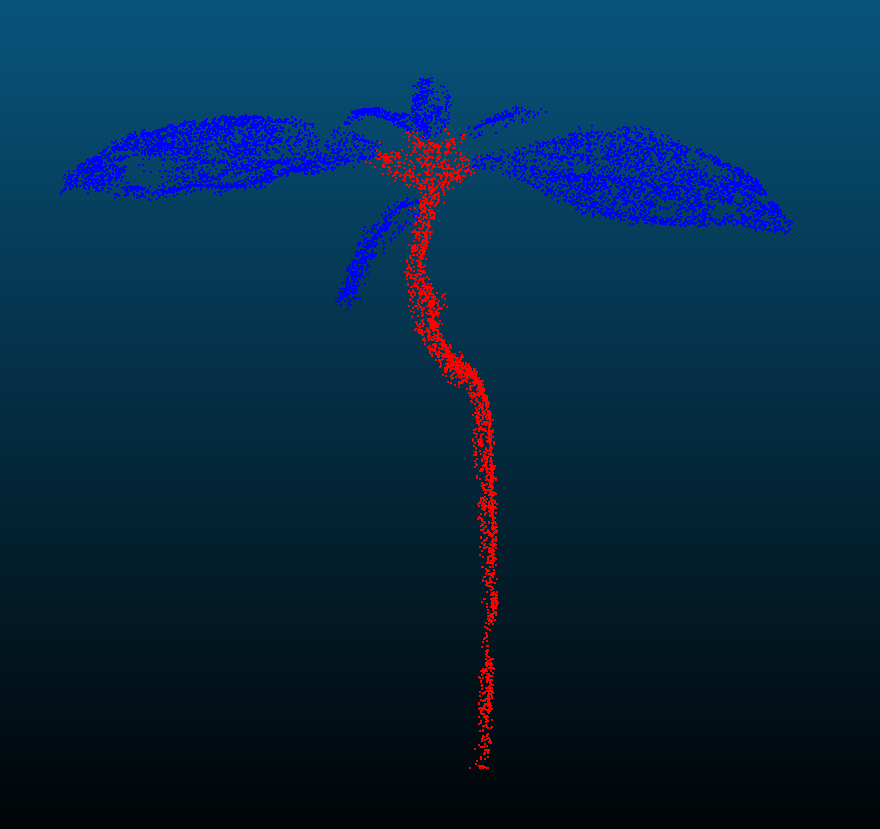
\includegraphics[width=\linewidth]{./Images/Plant_Avocado.png}
  \caption{Avocado}
  \label{fig:segmentation:compare:1}
\end{subfigure}\hfil
\begin{subfigure}{0.24\textwidth}
  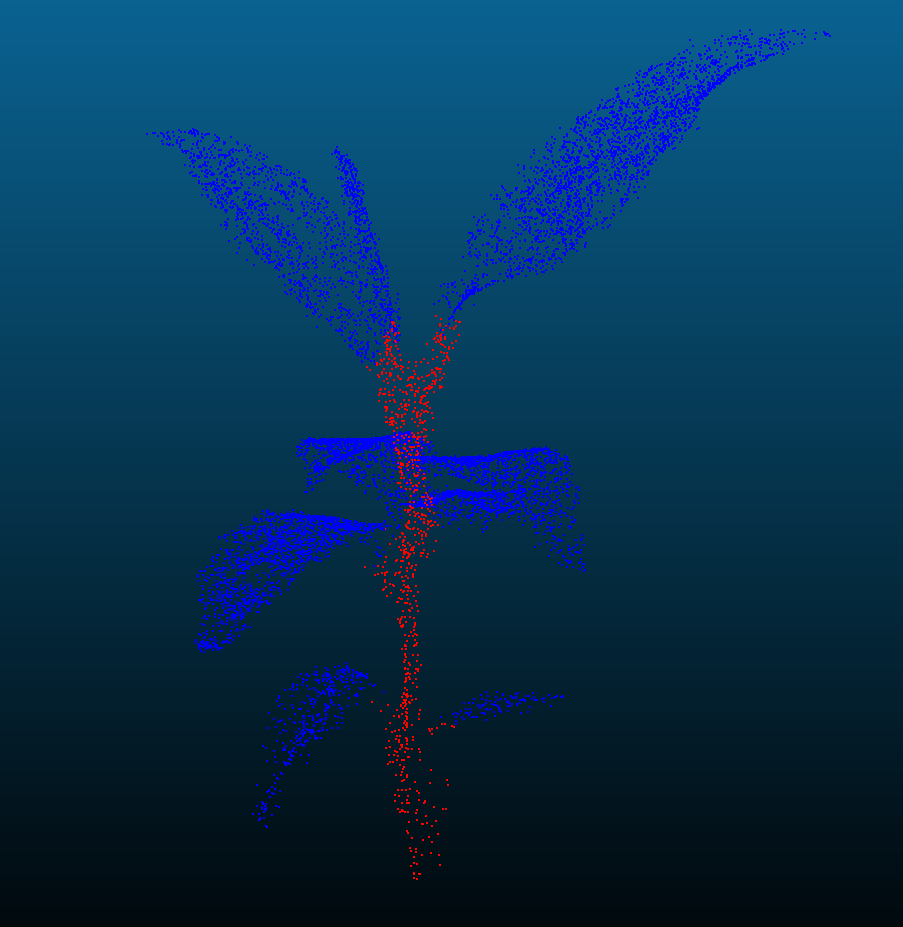
\includegraphics[width=\linewidth]{./Images/Plant_Banana.png}
  \caption{Banane}
  \label{fig:segmentation:compare:2}
\end{subfigure}\hfil
\begin{subfigure}{0.24\textwidth}
  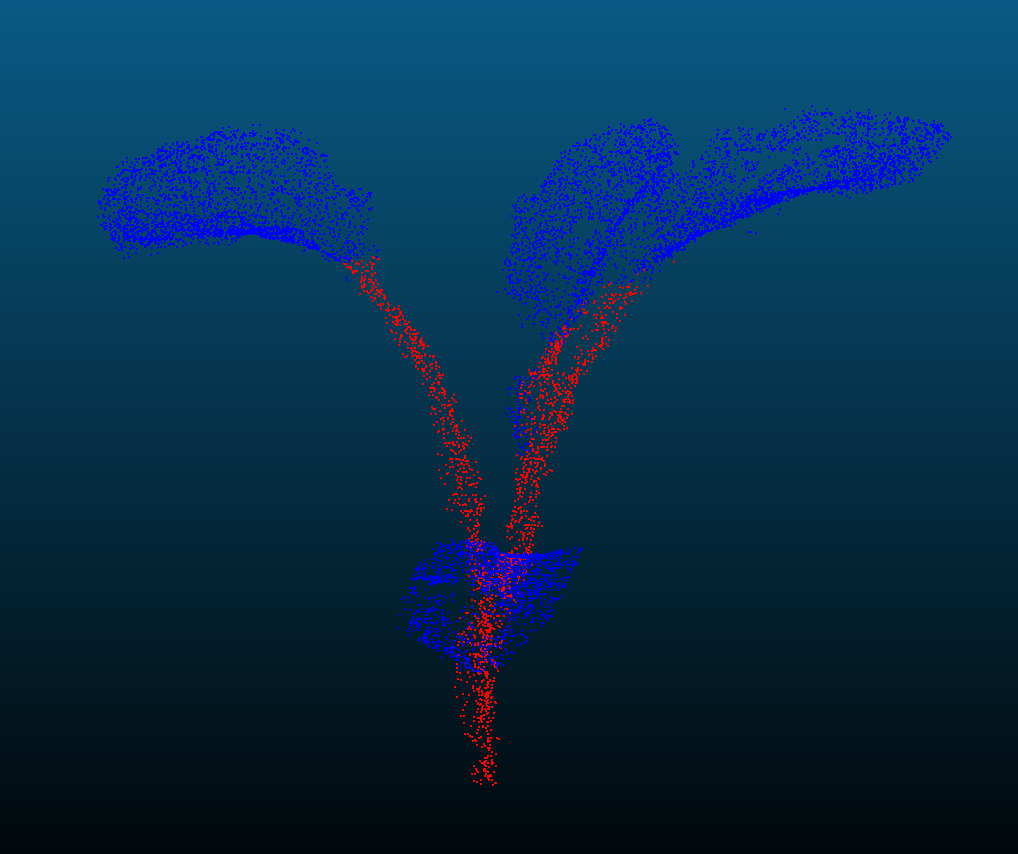
\includegraphics[width=\linewidth]{./Images/Plant_Kohlrabi.png}
  \caption{Kohlrabi}
  \label{fig:segmentation:compare:3}
\end{subfigure}\hfil
\begin{subfigure}{0.24\textwidth}
    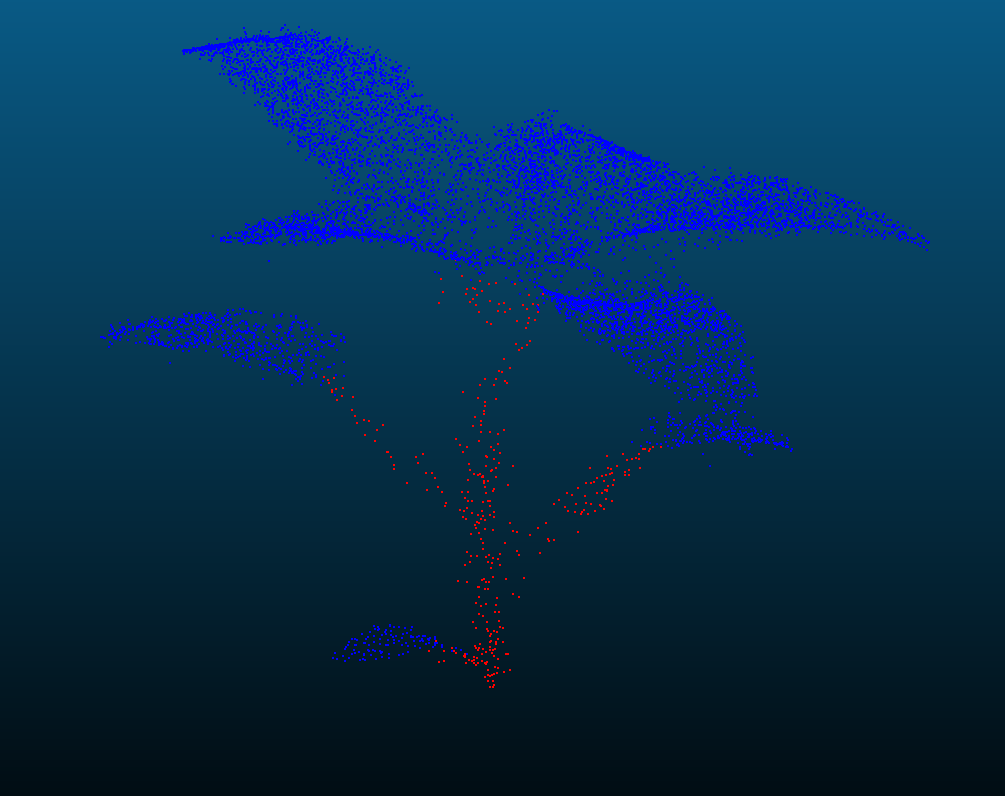
\includegraphics[width=\linewidth]{./Images/Plant_Paprika.png}
    \caption{Paprika}
    \label{fig:segmentation:compare:4}
  \end{subfigure}

\medskip
\begin{subfigure}{0.24\textwidth}
  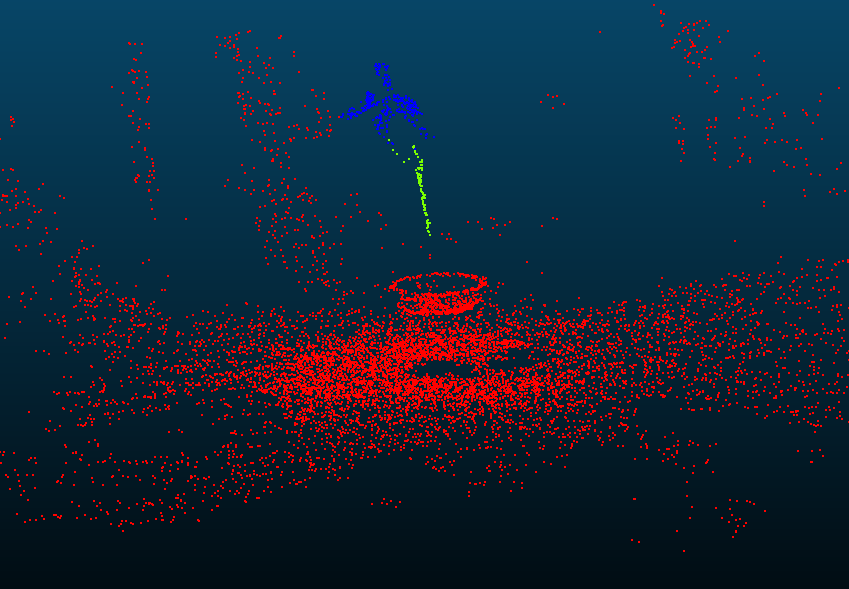
\includegraphics[width=\linewidth]{./Images/BG_Avocado.png}
  \caption{Avocado}
  \label{fig:segmentation:compare:5}
\end{subfigure}\hfil 
\begin{subfigure}{0.24\textwidth}
  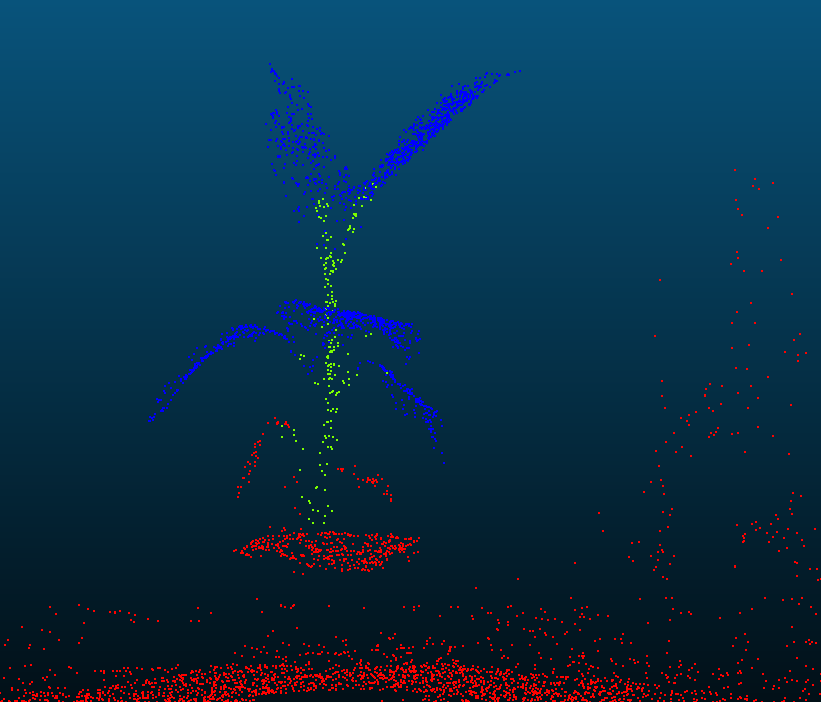
\includegraphics[width=\linewidth]{./Images/BG_Banana.png}
  \caption{Banane}
  \label{fig:segmentation:compare:6}
\end{subfigure}\hfil 
\begin{subfigure}{0.24\textwidth}
  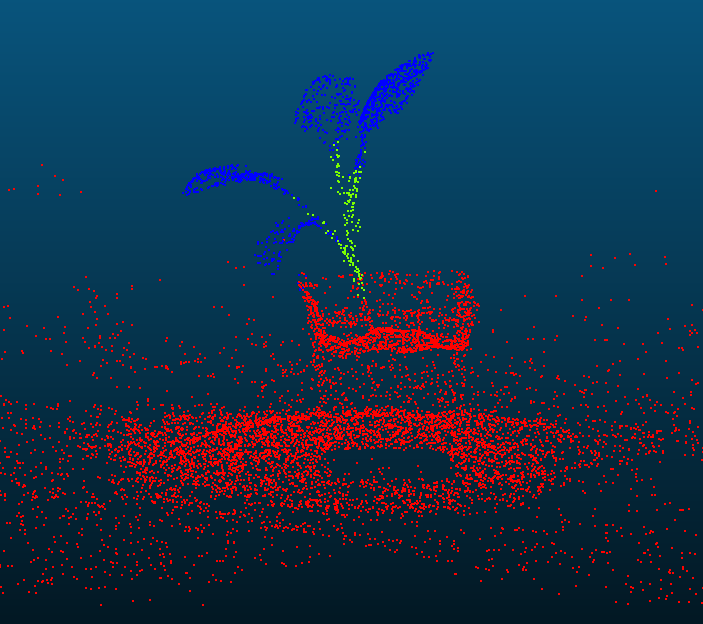
\includegraphics[width=\linewidth]{./Images/BG_Kohlrabi.png}
  \caption{Kohlrabi}
  \label{fig:segmentation:compare:7}
\end{subfigure}\hfil 
\begin{subfigure}{0.24\textwidth}
    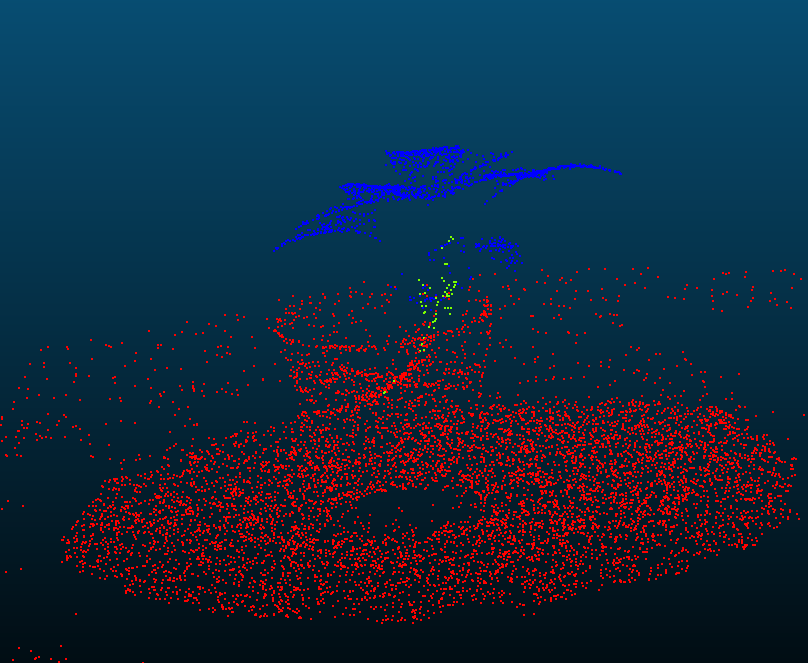
\includegraphics[width=\linewidth]{./Images/BG_Paprika.png}
    \caption{Paprika}
    \label{fig:segmentation:compare:8}
\end{subfigure}
\caption{Segmentierungsergebnisse für Vordergrund(a-d) und Hintergrund(e-h)}
\label{fig:segmentation:compare}
\end{figure}

\begin{table}
    \begin{center}
    \begin{tabular}{|l || c | c | c || c | c | c | c | c |} 
        \hline
         & \thead{t11}  & \thead{t6} & \thead{t10} & \thead{t9} & \thead{t4} & \thead{t7} & \thead{t12} & \thead{t13}  \\  
        \hline
        \hline
        Loss & $0,044$ & $0.056$& $0.079$& $0.05$& $0.038$& $0.054$& $0.051$& $0.127$\\
        \hline
        Genauigkeit & $0,98$& $0.976$& $0.969$& $0.982$& $0.986$& $0.981$& $0.98$& $0.95$\\
        \hline
        IoU & $0.925$& $0.908$& $0.893$& $0.811$& $0.813$& $0.788$& $0.841$& $0.827$\\
        \hline
    \end{tabular}
    \end{center}
    \caption{Evaluations-Ergebnisse der verschiedenen Netze. Links ohne Hintergrund. Rechts mit Hintergrund.}
    \label{tab:segmentation:eval}
\end{table}


\begin{figure}
    \centering
    \begin{minipage}{0.475\textwidth}
        \centering
        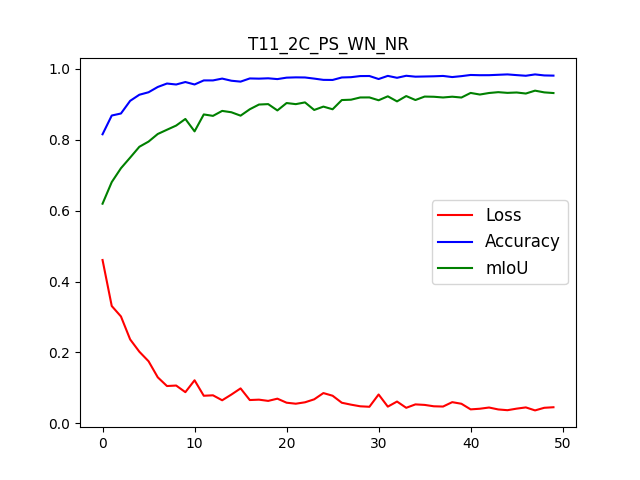
\includegraphics[width=1.0\textwidth]{./Images/T11_2C_PS_WN_NR.png}
        \caption{PointNet++ Trainings-Ergebnisse pro Epoche mit 2 Klassen und Normalisierung ohne zufällige Rotationen}
        \label{fig:T11_2C_PS_WN_NR}
    \end{minipage}\hfill
    \begin{minipage}{0.475\textwidth}
        \centering
        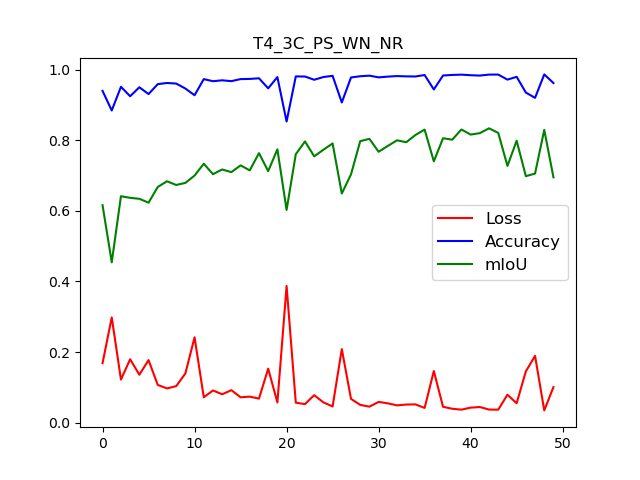
\includegraphics[width=1.0\textwidth]{./Images/T4_3C_PS_WN_NR.png}
        \caption{PointNet++ Trainings-Ergebnisse pro Epoche mit 3 Klassen und Normalisierung ohne zufällige Rotationen}
        \label{fig:T4_3C_PS_WN_NR}
    \end{minipage}
\end{figure}

\begin{figure}
    \centering
    \begin{minipage}{0.475\textwidth}
        \centering
        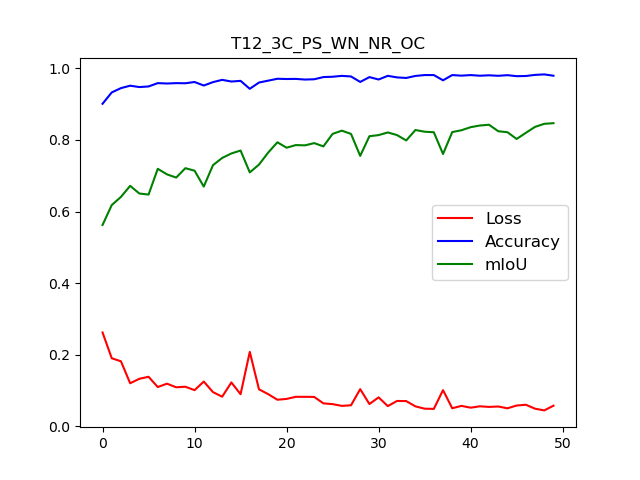
\includegraphics[width=1.0\textwidth]{./Images/T12_3C_PS_WN_NR_OC.png}
        \caption{PointNet++ Trainings-Ergebnisse pro Epoche mit 3 Klassen und Normalisierung ohne zufällige Rotationen. Mit Ausschnitt um das Zentrum.}
        \label{fig:T12_3C_PS_WN_NR_OC}
    \end{minipage}\hfill
    \begin{minipage}{0.475\textwidth}
        \centering
        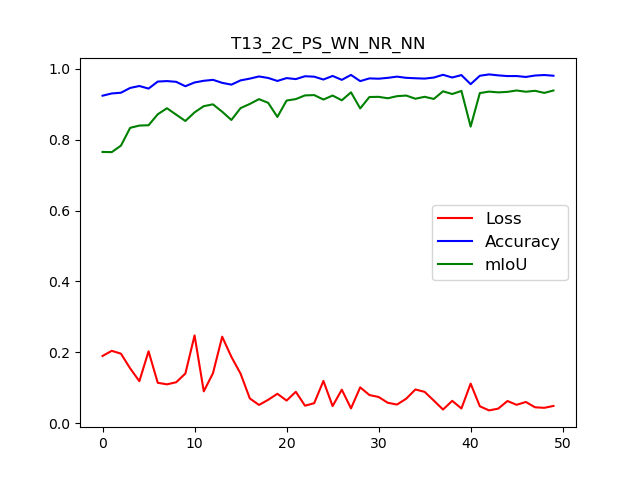
\includegraphics[width=1.0\textwidth]{./Images/T13_2C_PS_WN_NR_NN.png}
        \caption{PointNet++ Trainings-Ergebnisse pro Epoche mit 2 Klassen und Normalisierung ohne zufällige Rotationen. Ohne Normalen}
        \label{fig:T13_2C_PS_WN_NR_NN}
    \end{minipage}
\end{figure}

\textbf{Vergleich Training mit und ohne Normalen}

Um zu überprüfen, ob sich der Einsatz von Normalen lohnt, wird PointNet++ ohne Normalen trainiert und die Ergebnisse mit den Ergebnissen des Trainings mit Normalen (Abbildung \ref{fig:T11_2C_PS_WN_NR}) verglichen. 
Die Ergebnisse des Trainings ohne Normalen, in Abbilung \ref{fig:T13_2C_PS_WN_NR_NN} zu sehen, lassen einen kleinen Unterschied zum Training mit Normalen erkennen. 
Mit Normalen liefern die ersten Epochen zwar schlechtere Ergebnisse, aber nach einigen weiteren Epochen gleicht sich die Güte an und es kommt zudem zu weniger Ausreißern. 
Der Einsatz von Normalen scheint sich also in geringem Maß zu lohnen. 

\textbf{Vergleich Training mit und ohne Normalisierung} 

Es soll überprüft werden, ob PointNet++ mit oder ohne Normaliserung bessere Ergebnisse liefert. 
Des weiteren soll geprüft werden, ob auch nichtnormaliserte Eingabe-Daten gute Segmentierungs-Ergebnisse liefern, wenn PointNet++ mit normaliserten Daten trainiert wurde.
Dieser Vergleich wird aufgestellt, da die Punkwolken für die Segmentierung auf eine bestimmte Anzahl Punkte reduziert werden und das Ergebnis - zumindest bei der Hintergrund-Segmentierung - 
zurück auf die vollständige Punktwolke übertragen werden muss.
%Dafür darf die reduzierte Punktwolke ihre Position nicht ändern. Um das zu gewährleisten muss die Normalisierung die PointNet++ ausführt verhindert oder umgekehrt werden. 
Muss die Punktwolke nicht normalisert werden, kann das Ergebniss direkt auf die vollständige Punktwolke übertragen werden. 
Im Falle einer Normaliserung müsste diese erst umgekehrt werden, aber diese Information wird von PointNet++ nicht zur Verfügung gestellt und müsste ermittelt werden.
Alternativ dazu könnten auch die Ergebnisse von der normalisierten Punktwolke auf die nicht normaliserte Punktwolke übertragen werden, was aber mit mehr Rechenaufwand verbunden ist.

Wird die Normalisierung komplett verhindert, kann das Auswirkungen auf die Güte der Ergebnisse der Segmentierung haben.

\begin{table}
    \begin{center}
    \begin{tabular}{|l || c | c || c | c | } 
        \hline
         & \thead{t4 mit \\ normalisiert Daten}  & \thead{t4 mit nicht \\ normalisiert Daten} & \thead{t11 mit \\ normalisiert Daten} & \thead{t11 mit nicht \\ normalisiert Daten}  \\  
        \hline
        \hline
        Loss & $0,038$ & $0,175$& $0.044$& $0.044$\\
        \hline
        Genauigkeit & $0,986$& $0,946$& $0.98$& $0.98$\\
        \hline
        IoU & $0,81$& $0,684$& $0.926$& $0.925$\\
        \hline
    \end{tabular}
    \end{center}
    \caption{Vergleich von Evaluations-Ergebnissen von den mit normaliserten Daten trainierten Netzen t4 (mit Hintergrund) und t11(ohne Hintergrund) mit jeweils normalisierten und nicht normaliserten Daten.}
    \label{tab:segmentation:normalization:compare}
\end{table}

In Tabelle \ref{tab:segmentation:normalization:compare} werden die Ergebnisse der Evaluation von PointNet++ auf nicht normaliserten Daten nach dem Training mit normaliserten Daten verglichen.
Da die Ergebnisse sich für die Segmentierung mit Hintergrund stark verschlechtern, wenn die Daten nicht normalisiert werden wird PointNet++ ohne Normalisierung erneut trainiert. 
Die Ergebnisse für das erneute Training sind in Abbildung \ref{fig:T6_2C_PS_NN_NR} für zwei Klassen und in Abbildung \ref{fig:T7_3C_PS_NN_NR} für drei Klassen zu sehen.

\begin{figure}
    \centering
    \begin{minipage}{0.475\textwidth}
        \centering
        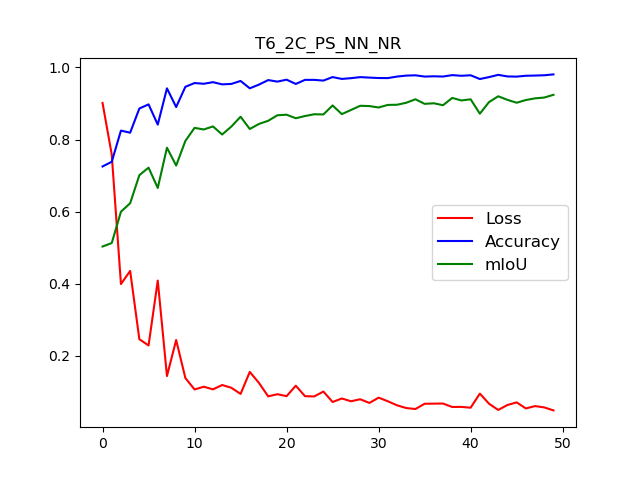
\includegraphics[width=1.0\textwidth]{./Images/T6_2C_PS_NN_NR.png}
        \caption{PointNet++ Trainings-Ergebnisse pro Epoche mit 2 Klassen, ohne Normalisierung und ohne zufällige Rotationen }
        \label{fig:T6_2C_PS_NN_NR}
    \end{minipage}\hfill
    \begin{minipage}{0.475\textwidth}
        \centering
        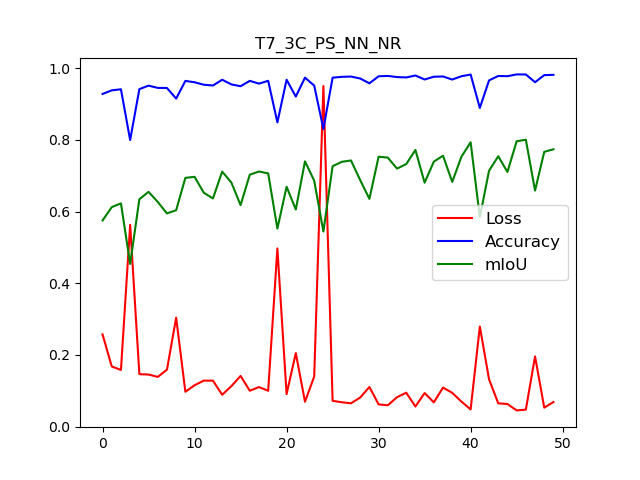
\includegraphics[width=1.0\textwidth]{./Images/T7_3C_PS_NN_NR.png}
        \caption{PointNet++ Trainings-Ergebnisse pro Epoche mit 3 Klassen, ohne Normalisierung und ohne zufällige Rotationen}
        \label{fig:T7_3C_PS_NN_NR}
    \end{minipage}
\end{figure}

Gegenüber dem Training mit Normalisierung ist das Training ohne Normalisierung etwas schlechter. Insbesondere für das Netz mit drei Klassen haben die Ausreißer für Loss-, Accuracy- und IoU-Werte zugenommen.
Das führt zu dem Schluss, dass PointNet++ mit Normalisierung genutzt werden sollte und der zusätzliche Rechenaufwand zum Übertragen der Ergebnisse auf die vollständige Punktwolke in kauf genommen werden sollte.

\textbf{Vergleich Training mit und ohne zufällige Rotationen}

Die Tests des Servers haben gezeigt, dass es bei der Segmentierung der freigestellten Pflanzen zu starken Fehlern kommt, wenn diese rotiert sind. 
Diese Fehler sind in Abbildung \ref{fig:rotation:error:1} und \ref{fig:rotation:error:2} zu sehen.
Wird die Evaluation eines ohne zufällig rotierte Punktwolken trainierten Netzes mit zufällig rotierten Punktwolken ausgeführt sinkt der IoU-Wert auf $0,6$ und Accuracy auf $0,875$
Da dieser Unterschied signifikant ist, ist davon auszugehen, dass PointNet++ anfällig für Rotationen ist, wenn diese im Training nicht berücksichtigt wurden.

Aus diesem Grund wurde das Training für das Zwei- und Drei-Klassen-Netz mit zufälligen Rotationen wiederholt um eine Robustheit gegen Rotationen anzutrainieren.
Die Ergebnisse für das Zwei-Klassen-Netz ist in Abbildung ~\ref{fig:10_2C_PS_WN_RR} zu sehen, die Ergebnisse für das Drei-Klassen-Netz in Abbildung ~\ref{fig:9_3C_PS_WN_RR}. 
Beim Training des Netzes mit drei Klassen sind starke Ausreißer in den Loss-Werten zu erkennen, die sich auch in der Accuracy und dem IoU - wenn auch nicht so stark - wiederspiegeln.
Diese Beobachtung kann man bei den anderen Netzen nur in wesentlich kleinerem Ausmaß feststellen. 
Dennoch sind die Ergebnisse für das Training mit zufälligen Rotationen wesentlich schlechter als die des Trainings ohne zufällige Rotationen.
Im Einsatz sollte also bei der Entfernung des Hintergrundes darauf geachtet werden, dass dieser zumindest grob an der XY-Ebene ausgerichtet ist.

\begin{figure}
    \centering
    \begin{minipage}{0.475\textwidth}
        \centering
        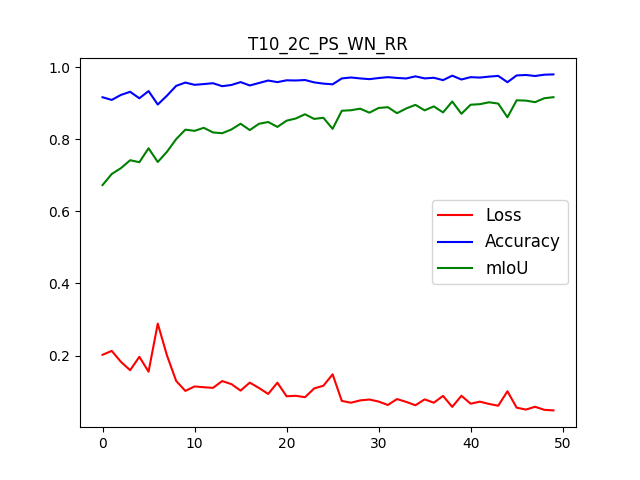
\includegraphics[width=1.0\textwidth]{./Images/10_2C_PS_WN_RR.png}
        \caption{PointNet++ Trainings-Ergebnisse pro Epoche mit 2 Klassen, mit Normalisierung und zufälliger Rotationen}
        \label{fig:10_2C_PS_WN_RR}
    \end{minipage}\hfill
    \begin{minipage}{0.475\textwidth}
        \centering
        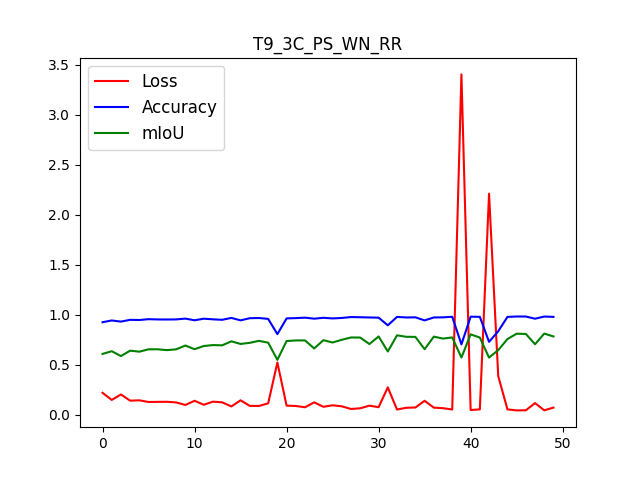
\includegraphics[width=1.0\textwidth]{./Images/9_3C_PS_WN_RR.png}
        \caption{PointNet++ Trainings-Ergebnisse pro Epoche mit 3 Klassen, mit Normalisierung und zufälliger Rotationen}
        \label{fig:9_3C_PS_WN_RR}
    \end{minipage}
\end{figure}

\begin{figure}
    \centering
    \begin{minipage}{0.475\textwidth}
        \centering
        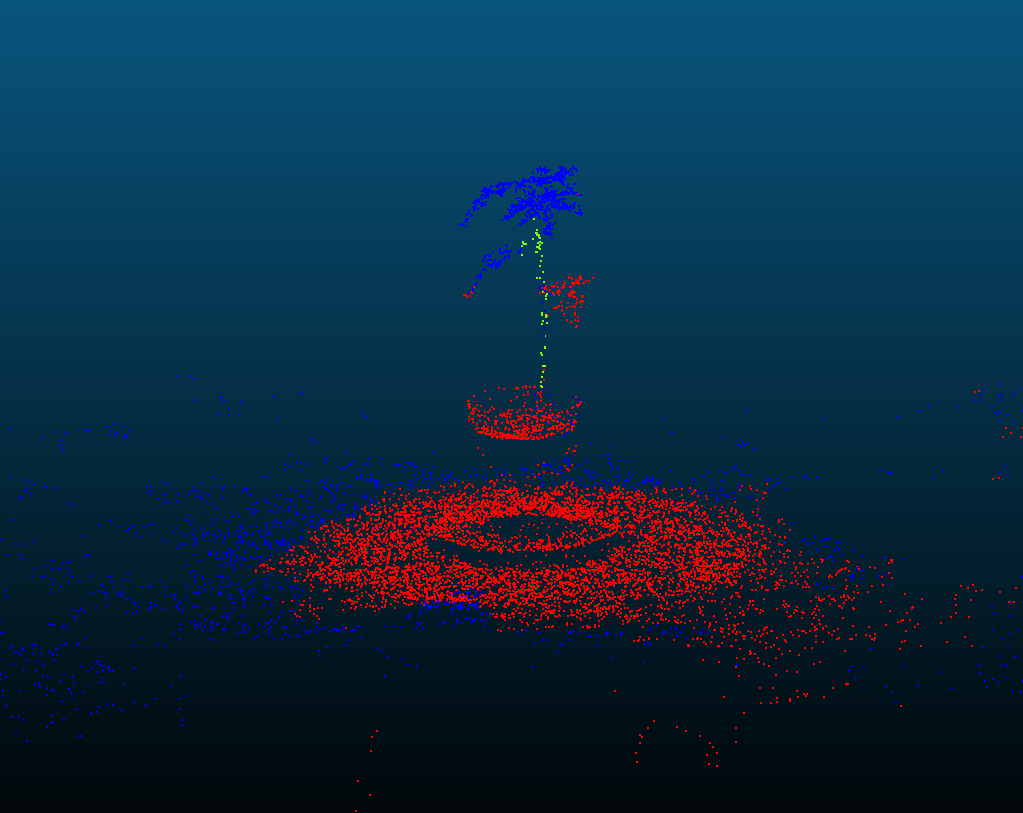
\includegraphics[width=1.0\textwidth]{./Images/RotationError1.png}
        \caption{Fehlgeschlagene Segmentierung einer Bananen-Pflanze. Verursacht durch Rotation der Punktwolke}
        \label{fig:rotation:error:1}
    \end{minipage}\hfill
    \begin{minipage}{0.475\textwidth}
        \centering
        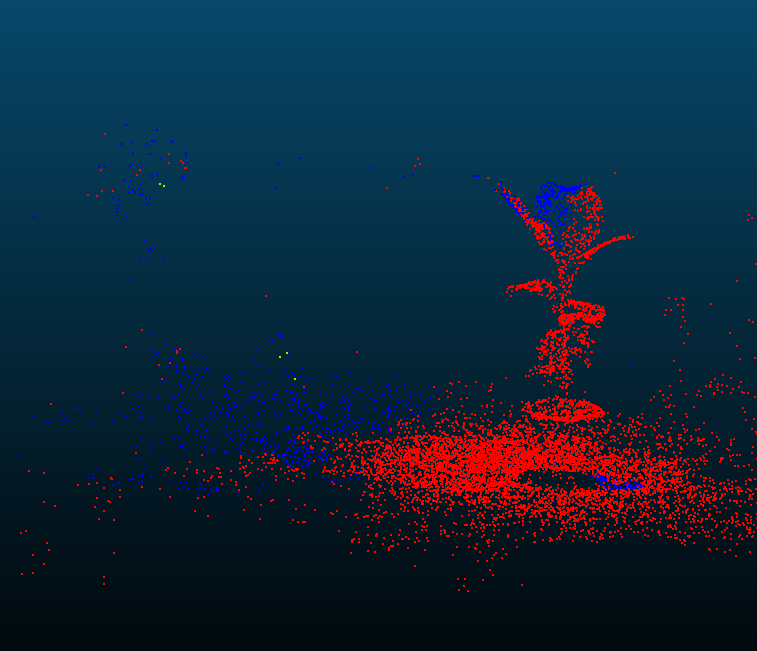
\includegraphics[width=1.0\textwidth]{./Images/RotationError2.png}
        \caption{Fehlgeschlagene Segmentierung einer Tomaten-Pflanze. Verursacht durch Rotation der Punktwolke}
        \label{fig:rotation:error:2}
    \end{minipage}
\end{figure}

\newpage
\section{Fazit und Ausblick}
%-------------------------------------------------------------
\label{sec:fazit}
%Am Ende der Arbeit muss ein Fazit dessen was geleistet wurde
%und wie es weitergehen kann. Dazu gehört auch wie der aktuelle
%Stand Ihrer Implementierung ist: ist Ihre Lösung z.B. bereits
%produktiv im Einsatz? Welche wesentlichen Punkte müssen noch
%umgesetzt werden?
%
%Insbesondere müssen hier die Schwachpunkte
%Ihrer Lösung erwähnt werden, also was Sie anders machen würden,
%wenn Sie dieselbe Aufgabe noch einmal bekämen. Auch nicht gelöste
%oder sich im Laufe der Arbeit neu ergebene Fragen müssen hier zur
%Sprache kommen.

\textbf{Generierung der Punkwolken}

Die Generierung von Punktwolken mit ODM liefert zwar gute Ergebnisse und ist vergleichsweise schnell. Allerdings ist es dennoch die Komponente, die am meisten Laufzeit in Anspruch nimmt.
Da keine Geo-Informationen zu den Bilder vorliegen, kann die GPU von ODM nicht eingesetzt werden. 
An der Stelle könnte ODM erweitert werden und die alternative Implementierung die ohne Geo-Informationen auskommt, könnte parallelisiert werden.

Sollte sich in Zukunft bei Smartphones eine RGB-D Kamera als Standart etablieren, könnte diese Technologie genutzt werden um eine schnelle Generierung der Punktwolken zu ermöglichen.
Wobei hier zu beachten wäre, dass es bei schwankenden Belichtungs-Verhälnissen zu Problemen kommen kann. 

Ein weiterer Ansatz der untersucht werden könnte, ist die Generierung von Punktwolken mit Neuronalen Netzen. Hier gibt es einige interessante Ansätze, die im Rahmen dieser Arbeit nicht untersucht wurden. 
Diese Ansätze ermöglichen es, aus einem Bild eine Punktwolke zu generieren, was dem Ziel, die zu übertragende Datenmenge gering zu halten, entgegen kommt. 
Dazu würden sie vorraussichtlich nach dem Training schnellere Laufzeiten als ODM liefern.
Einen Nachteil den die Implemtationen haben ist das diese meist nur wenige $1000$ Punkte effizent liefern können, was zu SfM-Implementation wie ODM einen Nachteil darstellt. 
Dieses kann je nach Datenbasis einige $100000$ Punkte berechnen. Hier könnten aber mehrere Punktwolken erstellt werden und miteinender registriert werden um diesen Nachteil zu kompensieren.

\textbf{Registrierung}

Die Ergebnisse der Registrierung sind zwar für den Zweck ausreichend, könnten aber zuverlässiger und genauer sein. Insbesondere die nicht bekannte Skalierung bereitet Probleme.

Bei der Datengewinnung könnte zu den Bildern auch eine GPS-Position ermittelt werden und auf diese Weise Punktwolken mit gleichem Maßstab erstellt werden. 
Das würde die Registrierung erleichtern, da die Skalierung nicht mehr geschätzt werden müsste.
Zudem könnte so die exakte Größe der Pflanze berechnet werden und damit auch der totale Größenunterschied zwischen zwei Wachstums-Zeitpunkten einer Pflanze.
Zudem würde die Generierung der Punktwolken mit ODM beschleunigt, da die GPU von ODM genutzt werden könnte.

Ein weiterer Ansatz, der in dieser Arbeit nicht verfolgt wurde, ist ScaleLK. 
ScaleLK hat eine ähnliche Architektur wie PoinNetLK, allerdings wird neben Rotation und Translation auch eine Schätzung für die Skalierung geliefert.

Ein letzter Ansatz, der nicht zur Gänze untersucht wurde ist es RPM-Net mit dem Ansatz in \cite{Ziner2005PointSR} zu verbinden.
Hierbei wird die Archtiektur von RPM belassen, allerdings wird, nach dem Rotation bekannt ist, die Skalierung, wie in den Gleichungen \ref{eq:icp_scale:1} - \ref{eq:icp_scale:2} beschrieben, berechenet.
Des weiteren muss die Berechnung der Translation angepasst werden. Für das Training des angepassten Netzes muss auch die Trainings-Daten überarbeitet werden.
Zu jedem Trainings-Datensatz muss eine zuällig Skalierung hinzugefügt werden. Dieses Vorgehen wurde im Ansatz implementiert, aber nicht weiter untersucht.

\textbf{Segmentierung}

Die Segmentierung ist für die Hintergrundentfernung noch recht fehleranfällig. Hier könnte probiert werden, mit einem größerem Datensatz zu trainieren, 
mehr Punkte während des Trainings zu nutzen oder - wie untersucht - nur einen Ausschnitt um das Zentrum der Punktwolke segmentieren.

Der untersuchte Ansatz, einen Ausschnitt aus der Szene um dessen Zentrum zu nehmen, wirkt sich zwar positiv auf die Ergebnisse aus, aber wird im praktischem Einsatz auf das Problem stoßen, 
dass nicht garantiert werden kann, dass der relevante Teil der Szene ausgeschnitten wird.
Statt dessen könnte die Szene als ganzes im Vorfeld untersucht werden und so relevante Bereiche ermittelt werden. 
Szenen-Segmentierung ist mittels Point-Net++ möglich, hier müssten nur geeignete Daten gesammelt werden, die dem Einsatz in der Realität entsprechen. 
So könnten auch einzelne Pflanzen isoliert untersucht werden und der Einfluss, den die Pflanzen beim Wachstum aufeinander haben, untersucht werden.
Neben Nutzpflanzen könnten bei einer Szene-Segmentierung auch Unkräuter erkannt werden und deren Wachstum, unter bestimmten Bedingungen, analysiert werden.

Des weiteren kann die Segmentierung der Pflanze erweitert werden um zusätzliche Informationen über eine Pflanze zu erhalten. 
Zum Beispiel können neben Blättern und Stielen auch Blüten und Früchte erkannt werden, was für die Analyse des Ertrags einer Fruchtfolge genutzt werden könnte.
Um das zu bewerkstelligen muss für jedes Merkmal ein weiters Label hinzugefügt werden und die Datenbasis, die für das Training genutzt wird, um Punktwolken erweitert werden, die diese Merkmale auch beinhalten.

Bisher wurden beim Training die Farben nicht mit einbezogen. Auch diese könnten zusätzlich genutzt werden um weitere Informationen, wie den Zustand einzelner Segmente der Pflanze, zu erkennen. 
Die Farbe kann bei Früchten Aufschluss über den Reifegrad geben und bei Blättern und Stamm Anzeichen von Krankheiten erkennen lassen.

\textbf{Server}

Um die Perfomance des Servers zu steigern könnte für die in c++ implementierten Funktionalitäten ein Python-Binding erstellt werden oder in Python-Code portiert werden. Bisher werden diese Funktionen über System-Kommandos angesteuert. 
Mit einem Python-Binding oder einer entsprechenden Portierung könnten diese direkt aus dem Python-Code angesprochen werden. 
Dadurch könnten die Daten zwischen den einzelnen Pipelines im Hauptspeicher gehalten werden und müssten nur noch zu Persistierungs-Zwecken auf der Festplatte abgelegt werden.

Da der Server keine Sicherheitsmechanismen zur Verfügung stellt, ist von einem Einsatz in der Praxis in diesem Zustand abzuraten. Es sollte mindestens ein User-Management hinzugefügt werden um die Schnittstellen vor Missbrauch zu schützen.

%Weitere Analyse der Daten

\newpage
% Literaturverzeichnis
%-------------------------------------------------------------
\addcontentsline{toc}{section}{Literatur}

\bibliographystyle{ieeetr}
\bibliography{./bibleografie.bib}

\end{document}